\documentclass[12pt]{article}
\usepackage[margin = 1.5in]{geometry}
\usepackage{tikz}
\usepackage{xcolor}
\usepackage{amsthm}
\usepackage{amsmath}
\usepackage{physics}
\usepackage{amssymb}
\usepackage{mathtools}
\usepackage{amsfonts}
\usepackage{comment}
\usepackage{subcaption}
\usepackage{graphicx}
\usepackage{setspace}
\usepackage{soul}
\usepackage{subfiles}
\usetikzlibrary{decorations.pathreplacing,calligraphy}
\title{{The Volatility of Marginal Information Rents}\\ {in Dynamic Mechanism Design}}
%\title{A Martingale Approach to Dynamic Mechanism Design}
%\title{Volatility and Incentives in Dynamic Mechanism Design}
\author{Daniel Chen\footnote{Assistant Professor of Economics, Princeton
University; dtchen@princeton.edu. \\
First version: August 5, 2026. I am grateful
to Mira Frick, Ryota Iijima, and Juuso Toikka for valuable discussions.}}
\date{\today}
%\\ \bigskip \href{https://danieltchen.com/volatility.pdf}{{Click here for the latest version}}
\usetikzlibrary{shapes.geometric}
\newtheorem{definition}{Definition}
\usepackage{natbib}
\newtheorem{claim}{Claim}
\newtheorem{theorem}{Theorem}
\newtheorem{lemma}{Lemma}
\newtheorem{corollary}{Corollary}[theorem]
\newtheorem{prop}{Proposition}
\newtheorem{conj}{Conjecture}
\newtheorem{condition}{Condition}
\newtheorem{example}{Example}
\newtheorem{remark}{Remark}
\newtheorem*{remark*}{Remark}

% --- subtheorem machinery: theorem parts print as 1a, 1b, ... ---
\newtheorem{subthm}{Theorem}
\renewcommand{\thesubthm}{\arabic{theorem}\alph{subthm}}
\newcommand{\nexttheoremset}{\refstepcounter{theorem}\setcounter{subthm}{0}}
% usage: call \nexttheoremset once, then use {subthm} for each part
% -------------------------------------------------------------------------------

\DeclareMathOperator*{\argmax}{arg\,max}
\usepackage{url}
%\definecolor{customgreen}{rgb}{0.00,0.4,0.18}
\definecolor{linkblue}{HTML}{1A3D7C}
\definecolor{customgreen}{HTML}{0B5D3B}
\usepackage{float}
\usepackage{xr-hyper}
\usepackage{xcolor}
\definecolor{linkred}{rgb}{0.55,0.05,0.05}
%\usepackage[colorlinks=true,
            %linkcolor=customgreen,
           % citecolor=customgreen,
           % urlcolor=customgreen]{hyperref}
%\usepackage{hyperref}
%\hypersetup{
%citebordercolor={1 1 1}
  %  }
  \usepackage[colorlinks=true,
            linkcolor=customgreen,
            citecolor=customgreen,
            urlcolor=customgreen]{hyperref}
\renewcommand*{\theHsubthm}{\arabic{theorem}.\arabic{subthm}}
\usepackage{scalerel,stackengine,amsmath}
\usepackage{bbm}
\usepackage{booktabs}
\usepackage{longtable}
\usepackage{array}
\usepackage{xcolor}
\DeclareMathOperator{\drift}{drift}
\DeclareMathOperator{\vol}{vol}
\newcommand{\E}{\mathbb{E}}
\newcolumntype{S}{>{\centering\arraybackslash$}m{0.18\textwidth}<{$}}
\newcolumntype{M}{>{\raggedright\arraybackslash}m{0.62\textwidth}}
 \newcommand{\cat}[1]{\midrule\multicolumn{2}{l}{\textbf{#1}}\\\midrule}
 \newcommand{\indep}{\perp\!\!\!\perp}

 \newcommand{\hth}{\hat\theta}
\newcommand{\hB}{\hat B}
\newcommand{\Et}{\mathbb{E}_t}
\usepackage{microtype}
\usepackage{enumitem}
\newcommand{\R}{\mathbb R}


\begin{document}

\hypersetup{pageanchor=false}
\maketitle

\begin{abstract}
This paper brings martingale methods of continuous-time contracting
to Myersonian dynamic mechanism design. In a benchmark setting, I show that
implementability is characterized by the volatility of the agent's
\emph{marginal information rent}---how the marginal rent responds to
innovations in his type. Once transfers satisfy the usual envelope
conditions, truthful reporting after the initial report is locally incentive compatible if
and only if the discounted volatility is a nonnegative
supermartingale. When the volatility has finite variation, the same
condition is necessary and sufficient for global incentive
compatibility after the initial report. Using this characterization, I cast the design problem
as optimal control, which applies even when the first-order approach
fails: one program solves for the optimal mechanism in a regular finite-variation class, and another for the optimal locally incentive-compatible
mechanism. The two bracket the designer’s true payoff. I apply the
results to financial market design (a monopolistic dealer, then an exchange). 
\end{abstract}
\bigskip

{Keywords:} dynamic mechanism design, contracts, persistent private information,
optimal control, market design, market microstructure
\thispagestyle{empty}
\clearpage


\newpage
\pagestyle{plain}
\pagenumbering{arabic}
\hypersetup{pageanchor=true}

\section{Introduction}

Dynamic mechanism design in the Myersonian tradition has developed largely in discrete time
\citep{courty2000sequential,battaglini2005longterm,eso2007optimal,pavan2014dynamic}.\footnote{An
exception is \citet{bergemann2015dynamic}, who solve dynamic
revenue-maximization problems in continuous time within the first-order
approach, using continuous-time versions of the envelope methods from
the discrete theory.} By contrast, dynamic contracting more broadly has benefited from continuous-time martingale methods \citep{demarzo2006optimal,sannikov2008,williams2011persistent}.
The two literatures study closely related problems (the first with transferable utility, the second without)
but have used surprisingly distinct methods. This paper extends martingale
methods to the Myersonian setting and studies how the two literatures' approaches relate. In the process, the paper obtains new results for both literatures.


The main result characterizes implementability in terms of a core object: the
volatility of the agent's marginal information rent---the sensitivity of the marginal rent
to innovations in his type. Once transfers satisfy the usual envelope
conditions, truthful reporting after the initial report is locally
incentive compatible if and only if the volatility is nonnegative and,
suitably discounted, a supermartingale under truthful reporting. When
the volatility has finite variation, the same conditions are necessary
and sufficient for global incentive compatibility after the initial
report.  The characterization also applies without
transfers and is thus new to both literatures, for reasons discussed below.\footnote{In brief, the canonical reference for contracting with adverse selection,
\citet{williams2011persistent}, restricts the agent to negative drift
distortions, whereas I allow distortions of either sign.} Because the
supermartingale condition is local in time, the design problem admits techniques from optimal control. Taken together, the results offer a complete characterization of locally
incentive-compatible mechanisms,\footnote{Local incentive compatibility, defined formally in Definition~\ref{def:local-ic},
rules out a payoff gain at quadratic order along every feasible
deviation direction. Technically, when that effect is zero, a small deviation may be profitable due to higher-order effects on payoffs. Under the conditions of
Appendix~\ref{app:strict-local}, the mechanism can be perturbed at
arbitrarily small cost to the designer so that the quadratic effect is
strictly negative in every nonzero direction.} identify a
natural class on which the characterization is global, and provide a method for optimizing over each class. I apply
the method to a classic problem in financial-market-design where the standard
first-order approach fails.

In the benchmark model, a principal chooses an allocation for a single
agent, charges transfers, and may bear a convex cost of provision. The
agent's marginal value for the allocation, his private type, follows a Markov diffusion. We assume the type follows an Ornstein--Uhlenbeck (OU) process but later extend to the case of a geometric Brownian motion (GBM).
The principal adjusts the allocation and transfers in response to the agent's \emph{reported} type path. The agent freely chooses his initial report and then controls the report's drift thereafter. The agent's
\emph{marginal information rent} is
the derivative of his continuation utility with respect to his current type under truthful reporting. By the envelope theorem, it equals the expected
discounted allocation stream, weighted by the impulse response of the
type process (see \eqref{eq: marginal rent}).


The marginal rent can be represented as an It\^{o} process with a drift and volatility. I show that implementability after
the initial report rests entirely on this volatility (Theorem~\ref{thm:after}, Lemma \ref{lem:master}). Local incentive compatibility is equivalent to volatility being a nonnegative supermartingale after discounting and moreover, implies global incentive compatibility when the volatility is of finite variation. At the initial report, local incentive compatibility is characterized by a comparison between initial volatility and the slope of the marginal rent schedule (that is, marginal rent as a function of the initial type); under a mild technical condition, global incentive compatibility in the finite-variation class is equivalent to an integral condition comparing initial volatility with the marginal rent schedule (Theorem~\ref{thm:zero}).


This characterization makes the principal's problem amenable to optimal control with the current report, the marginal rent,
and volatility as state variables. I formulate two programs that bracket the principal's true payoff: one program optimizes over finite-variation
mechanisms satisfying the date-zero integral condition and gives an
implementable lower bound; the other optimizes over locally
incentive-compatible mechanisms and gives an upper bound. 
In both programs, I use dynamic programming to characterize the principal's optimal continuation after time zero. Given the resulting value function, the principal selects the initial marginal rent and volatility schedules to solve a convex program. The finite-variation class is natural for two reasons: 1) it is the largest class for which all higher-order effects of deviations vanish, and 2) it is closely related to ``linear
mechanisms'' in discrete time (in a sense described shortly), in which the marginal rent is
linear, at each date, in the agent’s current report.


The two programs are applicable even when the first-order approach, whose validity requires strong assumptions \citep{pavan2014dynamic,battaglini2019optimal}, fails.  In those cases, both programs preserve the central
dynamic tradeoff the designer must then balance between limiting rents due to information today  versus creating surplus (to extract) from flexibility to respond to future innovations in the type. In
the environments covered by the irrelevance theorem
of \citet{eso2017dynamic}, this tradeoff disappears when the
first-order approach is valid: the designer earns as much as if the
agent's future types were observed directly. Analysis of the invalid case is thus economically
important, and this paper provides one route into it \citep{pavan2017dynamic}.

I also show how the analysis connects to the discrete-time theory. There,
incentive compatibility amounts to the envelope condition together with
\emph{integral monotonicity} \citep{pavan2014dynamic}: truthful reporting must
dominate every one-shot misreport in an integrated sense
(Section~\ref{sec:background}). Integral monotonicity, however, is
non-local and well known to be intractable to impose, both computationally and
analytically. I consider ``linear mechanisms'' in which the marginal rent responds linearly to the innovation in the type in each period. The loading on the innovation is predictable: it may depend on all past reports but
is fixed before the innovation is realized. These loadings are the
discrete-time analog of the marginal rent volatility. I show that integral monotonicity after the initial report collapses by elementary algebra to a
pointwise bound on the growth in loadings: the finite-difference form of drift condition in the finite-variation case. Also an exactly analogous integral condition disciplines the initial report. This is the sense in which ``linear mechanisms'' are the discrete-time counterpart of continuous-time finite-variation mechanisms, giving the finite-variation class a concrete interpretation 
(Section~\ref{sec:discrete-early}).



The incentive-compatibility characterization does not rely on transfers,
so it extends beyond the Myersonian setting
(Proposition~\ref{prop:no-transfers}). To my knowledge, this result is
also new to dynamic contracting more broadly. The key difference from
existing work is the set of deviations. The canonical reference,
\citet{williams2011persistent}, restricts the agent to negative drift
distortions. This one-sided restriction makes truthful reporting a
boundary choice and supports the first-order analysis common in that
literature. The
restriction prevents the agent from ever correcting a lie, and its economic
motivation is perhaps unclear \citep{bloedel2023persistent}. I allow drift distortions of either sign, so truthful
reporting is interior: first-order effects must vanish, and second-order
effects determine local incentives.





I apply the machinery to a classic setting in finance: a market maker trading
with a single trader whose hedging needs are private and persistent---a
dynamic version of the monopolistic dealer's problem
\citep{glosten1989insider}. I show that the first-order approach fails here outright
because the trader's side of the market is endogenous: whether he buys or sells
depends on the terms of trade. I solve the two control programs. Instead of the no-trade
interval a standard bid--ask spread would induce (and which arises under the first-order approach), the optimal mechanisms fill small
trading needs at reduced scale, balancing rent extraction today against surplus
extraction tomorrow. I then show that
a related design problem---a revenue-maximizing exchange in which many
traders participate and the market must clear---reduces to those
single-trader problems. The setting
belongs to a benchmark class of models in financial market microstructure, in
which traders bear quadratic holding costs
\citep[e.g.,][]{du2017optimal,malamud2017decentralized,chen2021fragmentation,antill2021augmenting}.




\paragraph{Related literature.}

The paper sits at the junction of two literatures: Myersonian dynamic mechanism
design and dynamic contracting more broadly. On the Myersonian side where the designer seeks to maximize revenue,\footnote{As opposed to the parallel strand on implementing efficient
allocations in dynamic environments; see \citet{bergemann2019introduction} for a
survey of both.} the field goes back to \citet{baron1984regulation} and
\citet{besanko1985multiperiod}. Contributions include \citet{courty2000sequential},
\citet{battaglini2005longterm}, \citet{eso2007optimal},
\citet{krahmer2011procurement}, and \citet{boleslavsky2013progressive}. \citet{pavan2014dynamic} give the general
treatment. \citet{pavan2017dynamic} and \citet{bergemann2019introduction} survey
this literature, which has primarily developed in discrete time.
I analyze this setting in continuous time, arriving at a distinct
characterization of implementability, and exploit tools from optimal control.
The closest paper is by \citet{bergemann2015dynamic},
who derive revenue-maximizing mechanisms in continuous time within the
first-order approach, by the envelope methods of the discrete theory; the present
paper instead confronts second-order incentives with martingale methods.

Within the Myersonian tradition, a recent line of work analyzes the failure of
the first-order approach directly.
\citet{battaglini2019optimal} show that with persistent types the failure is
generic. \citet{krasikov2021theory,krasikov2026dynamic} solve for optimal
contracts in specific environments where the approach fails;
\citet{garrett2015dynamic} and \citet{garrett2018robust} develop variational
methods that deliver optimality conditions and robust predictions without assuming
validity of the first-order approach; and
\citet{li2025stochastic} retain the local incentive constraints in a two-period
screening problem where the standard relaxation breaks down, showing
that stochastic mechanisms can then be essential. The control programs of
Section~\ref{sec:main_results} take a similar approach in an infinite-horizon
setting: the local
program optimizes subject to all local incentive constraints, while the
finite-variation program imposes global continuation incentive compatibility
together with a sufficient condition for truthful reporting at date zero. In
static settings, local first- and second-order
conditions are often sufficient for global incentive compatibility
\citep{carroll2012local}, but in dynamic settings no comparable result is
available.

On the contracting side, the paper extends the martingale methods of
continuous-time contract theory \citep{sannikov2008,williams2011persistent} to
screening with transfers and a nondegenerate initial type. The first-order
approach, however, is popular in contract theory, including the dynamic insurance
and public finance literature
\citep[e.g.,][]{zhang2009dynamic,kapicka2013efficient,farhi2013insurance}.
Most closely, \citet{williams2011persistent}
obtains sufficient conditions for incentive compatibility in a model
of dynamic insurance, with deviations restricted to negative drift distortions;
his conditions constrain the loading of the agent's promised marginal
utility---the counterpart, in his setting, of the rent volatility here. In contrast, I
consider drift distortions of either sign and obtain a characterization
of local incentive compatibility, which is fundamentally second order: with both
signs admitted, truthful reporting is interior rather than a corner of the
deviation set. 

This paper is partly inspired by \citet{bloedel2023persistent}, who revisit
Williams's model and identify issues in its analysis of incentive compatibility
and optimality. They go on to analyze a class of \emph{self-insurance
contracts}---contracts implementable as consumption--saving problems for the
agent---and show that the optimal one generically strictly dominates the contract
Williams had identified as optimal in his leading application. They also show that
the analysis has close discrete-time analogues. \citet{acciaio2023note} likewise
revisit Williams's model, characterizing incentive compatibility within parametric
families of contracts linear in the report.
%\footnote{\citet{acciaio2023note} also use ``linear contracts'' for
%salary rules that are affine in the reported path, with deterministic
%coefficients. These rules induce discounted allocation streams with
%deterministic volatility and therefore form a special case of the
%contracts I call linear. Here, the volatility need only be predictable
%and may depend on past reports.}



\paragraph{Outline.}
Section~\ref{sec:background} reviews the discrete-time characterization
of incentive compatibility and the first-order approach.
Section~\ref{sec:discrete-early} offers intuition for the main results in
discrete time through linear mechanisms. Section~\ref{sec:model} sets out
the continuous-time model. Section~\ref{sec:main_results} presents the
volatility characterization and the two control programs used to bound
the designer's payoff. Section~\ref{sec:application} applies the results
to financial market design---first the dealer, then the exchange.
Section~\ref{sec:extensions} extends the analysis to geometric Brownian
motion, contracts without transfers, discusses contracts beyond finite variation that are globally certifiable. Section~\ref{sec:conclusion} concludes.
% NOTE (Sep 2, Claude): outline assumes the linear-contracts section
% follows the application (Version A); adjust if Version B is adopted.

\section{Background}\label{sec:background}

This section informally reviews the characterization of incentive
compatibility for Markov environments in \citet{pavan2014dynamic}. Time is discrete,
\(t\in\{0,1,\dots\}\). The agent privately observes his type
\(\theta_t\), which follows a Markov process, and reports a type each
period.  A direct mechanism specifies an allocation
process \(X=\{X_t\}\) and a transfer process \(T=\{T_t\}\), with
\(X_t\) and \(T_t\) measurable with respect to the report history
through period \(t\). The agent's flow utility is
\(u(\theta_t,X_t)-T_t\), discounted by \(\beta\in(0,1)\) per period.

Using the Markov property, \(\theta_s\) can be
written as a function of \(\theta_t\) and the shocks
arriving between \(t\) and \(s\). The impulse response
\(I_{s,t}=\partial\theta_s/\partial\theta_t\) is the marginal effect
of the time-\(t\) type on the time-\(s\) type, holding those intermediate shocks
fixed. Consider a one-shot misreport: the agent's current type is
\(\theta_t\), he reports \(\hat\theta_t\), and he reports truthfully
thereafter. Let \(X^{\hat\theta_t}\) be the allocation stream that
follows. The marginal information rent following this report is
\begin{equation}\label{eq: marginal rent}
  D_t(\hat\theta_t,\theta_t)
  \;=\;
  \mathbb E\!\left[\sum_{s=t}^{\infty}\beta^{\,s-t}\,I_{s,t}\,
  u_\theta\bigl(\theta_s,X_s^{\hat\theta_t}\bigr)
  \,\Big|\,\mathcal F_t\right].
\end{equation}
This is the expected discounted stream of marginal utilities weighted
by the impulse response. \(D_t(\theta_t,\theta_t)\) is the on-path marginal rent.
Write \(W_t(\theta_t)\) for the agent's continuation payoff at a
truthful history under truthful reporting.

Specializing \citet[Theorems~1--3]{pavan2014dynamic} to our setting gives the following informal
characterization:
\begin{enumerate}
\item[(i)] \emph{Envelope.} Every incentive-compatible mechanism
satisfies
\[
  W_t'(\theta_t)=D_t(\theta_t,\theta_t)
\]
at each truthful history.

\item[(ii)] \emph{Integral monotonicity.} Under their regularity conditions, an allocation rule is implementable\footnote{Implementable means that some transfer rule
makes truthful reporting optimal at every history, on and off path,
which \citet{pavan2014dynamic} call a strongly truthful equilibrium.} if and only if,
at every truthful history and for every current type \(\theta_t\) and
alternative report \(\hat\theta_t\),
\begin{equation}\label{eq:pst-im}
  \int_{\hat\theta_t}^{\theta_t}
  \bigl[D_t(l,l)-D_t(\hat\theta_t,l)\bigr]\,\dd l
  \geq0.
\end{equation}
\end{enumerate}

Condition (i) is the envelope condition, the dynamic analogue of the
Myersonian payoff formula. Given the allocation, it pins down the
truthful continuation payoff, and therefore expected transfers, up to
a constant. By itself, it is only necessary and follows from local optimality. Condition (ii) is the
global restriction. For every one-shot misreport, it compares the
on-path and off-path marginal rents after integrating between the
report and the true type. This comparison incorporates the entire
continuation allocation rather than imposing period-by-period
allocation monotonicity.

The difficulty lies in condition (ii). The off-path marginal rent
depends on the full continuation allocation induced by each current
misreport. Imposing the condition therefore requires a continuum of
constraints at every history, current type, and alternative report,
coupled across periods through the continuation allocation. This makes
direct analytic and numerical optimization difficult. The first-order
approach instead optimizes subject only to condition (i) and then
checks condition (ii). 

% ======================================================================
% PLACEMENT COMPARISON (Sep 2): two drafts of the discrete-time section.
% VERSION B (below, immediately following the Background section) and
% VERSION A (after the
% application). Keep one, delete the other; if B wins, rename the
% -early labels and delete A. Both define the discrete grid and
% loadings; the duplication is temporary.
% ======================================================================

\section{Discrete-Time Preview: Linear Mechanisms}
\label{sec:discrete-early}

This section gives discrete-time intuition for the volatility
characterization. For the linear mechanisms defined below, integral
monotonicity reduces to a one-step bound after the initial report and
an integral condition at date zero.

Fix \(r>0\), \(\lambda\geq0\), \(\gamma>0\), and
\(\overline\theta\in\mathbb R\). Let the interval \(\Delta t>0\) between dates satisfy
\(1-\lambda\Delta t>0\), and set
\[
  \beta:=e^{-r\Delta t},
  \qquad
  \beta_\lambda:=\beta(1-\lambda\Delta t).
\]
The type follows the Euler scheme for an OU process:
\[
  \theta_{t+1}
  =
  \theta_t+\lambda(\overline\theta-\theta_t)\Delta t
  +\gamma\varepsilon_{t+1},
\]
where the innovations are independent across periods and of
\(\theta_0\), with mean zero and variance \(\Delta t\). The agent's flow
utility gross of transfers is \(\theta_tX_t\Delta t\), so \(u_\theta=X_t\Delta t\). The
impulse response from period \(t\) to period \(s\) is
\((1-\lambda\Delta t)^{s-t}\).

Let \(\hth_t\) denote the report in period \(t\). The innovation
inferred from two consecutive reports is
\begin{equation}\label{eq:dt-innovation-early}
  \hat\varepsilon_{t+1}
  :=
  \frac{
    \hth_{t+1}-\hth_t
    -\lambda(\overline\theta-\hth_t)\Delta t
  }{\gamma}.
\end{equation}
At each report history, let \(\E_t\) denote expectation treating the
reports received as truthful and assuming truthful continuation. Under
\(\E_t\), \(\hat\varepsilon_{t+1}=\varepsilon_{t+1}\) and so has mean zero. The marginal rent is
\begin{equation}\label{eq:dt-rent-recursion-early}
  D_t
  :=
  \E_t\left[
    \sum_{s=t}^{\infty}
    \beta_\lambda^{\,s-t}X_s\Delta t
  \right]
  =
  X_t\Delta t+\beta_\lambda\E_t[D_{t+1}].
\end{equation}
At a history that is
truthful through period \(t-1\) with report \(\hth_t\),
\(D_t=D_t(\hth_t,\hth_t)\) in the notation of
Section~\ref{sec:background}. For an initial report \(y\), write
\(D(y):=D_0\), so \(D(y)=D_0(y,y)\).

In the continuous-time
model of the next section, the martingale representation theorem
implies
\begin{equation}\label{eq:dt-rent-sde-early}
  \dd D_t
  =
  \bigl[(r+\lambda)D_t-X_t\bigr]\dd t
  +\psi_t\,\dd B_t
\end{equation}
for a predictable process \(\psi\). In general, there is no analogous representation theorem in discrete time.


\begin{definition}[Linear mechanism]\label{def:linear-contract-early}
A mechanism is \emph{linear}
%\footnote{\citet{acciaio2023note}
%also call their contracts ``linear.'' Their contracts induce
%discounted allocation streams with deterministic volatility and are
%therefore a special case of the contracts defined here. Here the
%volatility need only be predictable and may depend on report history.}
if there are loadings \(\psi_t\), measurable with respect to the report
history through period \(t\), such that
\begin{equation}\label{eq:dt-linear-dynamics-early}
  D_{t+1}
  =
  \frac{D_t-X_t\Delta t}{\beta_\lambda}
  +\psi_t\hat\varepsilon_{t+1}.
\end{equation}
\end{definition}

Taking \(\E_t\) in \eqref{eq:dt-linear-dynamics-early} recovers the
recursion in \eqref{eq:dt-rent-recursion-early}. The loading \(\psi_t\) is the
discrete counterpart of the continuous-time volatility \(\psi\). Moreover,
\(\beta_\lambda^{-1}=1+(r+\lambda)\Delta t+O(\Delta t^2)\), so
\(\E_t[D_{t+1}]-D_t\) coincides with
\(\bigl[(r+\lambda)D_t-X_t\bigr]\Delta t\) up to first order.

\begin{prop}\label{prop:linear-imc-early}
Let the mechanism be linear, with all marginal rents
\(D_t(\hth_t,\theta_t)\) well defined and finite.
Truthful reporting satisfies integral
monotonicity at every period \(t\geq1\) if and only if, at every
truthful history through period \(t-1\) and for every report in
period \(t\),
\begin{equation}\label{eq: discrete bound}
  \beta(1-\lambda\Delta t)^2\psi_t
  \leq
  \psi_{t-1}.
\end{equation}
At period \(0\), integral monotonicity holds if and only if
\begin{equation}\label{eq:discrete date zero}
  \int_y^x
  \left[
    D(l)-D(y)
    -\beta(1-\lambda\Delta t)^2
      \frac{\psi_0(y)}{\gamma}(l-y)
  \right]\dd l
  \geq0
  \qquad \forall x,y.
\end{equation}
\end{prop}

% OLD PROOF (recursion-based), commented out Sep 17 at DT's request.
\begin{comment}
\begin{proof}
Fix \(t\geq1\), a truthful history through period \(t-1\), and a
current type \(l\). Suppose the agent reports \(\hth_t\) and reports
truthfully thereafter. Write \(\psi_t(\hth_t)\) for the loading at this
history.

\emph{Past loading.} The paths with reports \(l\) and \(\hth_t\) in
period \(t\) share the history through period \(t-1\). By
\eqref{eq:dt-innovation-early}, their values of \(\hat\varepsilon_t\)
differ by \((l-\hth_t)/\gamma\), so
\eqref{eq:dt-linear-dynamics-early} at \(t-1\) gives
\begin{equation}\label{eq:dt-past-loading-early}
  D_t(l,l)-D_t(\hth_t,\hth_t)
  =
  \psi_{t-1}\,\frac{l-\hth_t}{\gamma}.
\end{equation}

\emph{Current loading.} Since reports are truthful from period
\(t+1\), \eqref{eq: marginal rent} gives
\begin{equation}\label{eq:dt-offpath-rent-early}
  D_t(\hth_t,l)
  =
  X_t\Delta t+\beta_\lambda\,\E\bigl[D_{t+1}\,\big|\,\theta_t=l\bigr],
\end{equation}
where \(D_{t+1}\) is evaluated on the path with report \(\hth_t\). On
this path, since
\(\theta_{t+1}=l+\lambda(\overline\theta-l)\Delta t+\gamma\varepsilon_{t+1}\),
\[
  \hat\varepsilon_{t+1}
  =
  \frac{\theta_{t+1}-\hth_t-\lambda(\overline\theta-\hth_t)\Delta t}{\gamma}
  =
  \varepsilon_{t+1}+(1-\lambda\Delta t)\frac{l-\hth_t}{\gamma}.
\]
Taking \(\E[\,\cdot\mid\theta_t=l]\) in
\eqref{eq:dt-linear-dynamics-early} at \(t\), where
\(D_t=D_t(\hth_t,\hth_t)\) on this path,
\[
  \E\bigl[D_{t+1}\,\big|\,\theta_t=l\bigr]
  =
  \frac{D_t(\hth_t,\hth_t)-X_t\Delta t}{\beta_\lambda}
  +\psi_t(\hth_t)(1-\lambda\Delta t)\frac{l-\hth_t}{\gamma}.
\]
Substituting into \eqref{eq:dt-offpath-rent-early} and using
\(\beta_\lambda(1-\lambda\Delta t)=\beta(1-\lambda\Delta t)^2\),
\begin{equation}\label{eq:dt-current-loading-early}
  D_t(\hth_t,l)-D_t(\hth_t,\hth_t)
  =
  \beta(1-\lambda\Delta t)^2\,\psi_t(\hth_t)\,\frac{l-\hth_t}{\gamma}.
\end{equation}
Subtracting \eqref{eq:dt-current-loading-early} from
\eqref{eq:dt-past-loading-early},
\[
  D_t(l,l)-D_t(\hth_t,l)
  =
  \Bigl[\psi_{t-1}-\beta(1-\lambda\Delta t)^2\psi_t(\hth_t)\Bigr]
  \frac{l-\hth_t}{\gamma}.
\]
Integrating over \(l\) from \(\hth_t\) to \(\theta_t\),
\[
  \int_{\hth_t}^{\theta_t}
  \bigl[D_t(l,l)-D_t(\hth_t,l)\bigr]\dd l
  =
  \frac{\psi_{t-1}-\beta(1-\lambda\Delta t)^2\psi_t(\hth_t)}{2\gamma}
  (\theta_t-\hth_t)^2,
\]
which is nonnegative for every \(\theta_t\) if and only if
\eqref{eq: discrete bound} holds at \(\hth_t\).

At date zero, let the true type be \(l\) and the report \(y\).
Equation \eqref{eq:dt-current-loading-early} holds with \(t=0\):
\[
  D_0(y,l)-D_0(y,y)
  =
  \beta(1-\lambda\Delta t)^2\,\psi_0(y)\,\frac{l-y}{\gamma}.
\]
Since \(D_0(l,l)=D(l)\) and \(D_0(y,y)=D(y)\), subtracting gives
\[
  D_0(l,l)-D_0(y,l)
  =
  D(l)-D(y)
  -\beta(1-\lambda\Delta t)^2
  \frac{\psi_0(y)}{\gamma}(l-y),
\]
and integrating from \(y\) to \(x\) yields \eqref{eq:discrete date zero}.
\end{proof}
\end{comment}

% Representation-based proof; the earlier recursion proof is retained above.
\begin{proof}
Fix a truthful history through \(t-1\), with \(t\geq1\). Condition
on this history and \(\theta_t=l\), and consider a one-shot deviation
to \(\hth_t\). Write \(\psi_t(\hth_t)\) for the loading after this
report. Iterating \eqref{eq:dt-linear-dynamics-early} forward gives\footnote{The
terminal term vanishes almost surely by the definition of \(D_n\) and
martingale convergence.}
\begin{equation}\label{eq:dt-linear-rep-early}
  \sum_{s=0}^{\infty}\beta_\lambda^{\,s}X_s\Delta t
  =
  D(\hth_0)
  +\sum_{s=0}^{\infty}\beta_\lambda^{\,s+1}\psi_s\hat\varepsilon_{s+1}.
\end{equation}
\begin{comment}
To justify the limit, let \(\mathcal F_n\) denote the actual history
through \(n\). For \(n\geq t+1\), finite telescoping gives the first
equality below; the rent definition and Markov property give the second,
since reporting has resumed truthfully:
\[
\begin{aligned}
  D(\hth_0)
  +\sum_{s=0}^{n-1}\beta_\lambda^{\,s+1}\psi_s\hat\varepsilon_{s+1}
  &=\sum_{s=0}^{n-1}\beta_\lambda^{\,s}X_s\Delta t
    +\beta_\lambda^{\,n}D_n\\
  &=\E\!\left[
    \sum_{s=0}^{\infty}\beta_\lambda^{\,s}X_s\Delta t
    \,\middle|\,\mathcal F_n\right].
\end{aligned}
\]
The allocation total is integrable by the marginal-rent definition.
Martingale convergence therefore gives \eqref{eq:dt-linear-rep-early},
with the innovation series converging almost surely and in \(L^1\).
This also justifies taking its conditional expectation.
\end{comment}

\noindent By \eqref{eq:dt-innovation-early}, the misreport changes only two
inferred innovations:
\[
  \hat\varepsilon_t
  =\varepsilon_t+\frac{\hth_t-l}{\gamma},
  \qquad
  \hat\varepsilon_{t+1}
  =\varepsilon_{t+1}+(1-\lambda\Delta t)\frac{l-\hth_t}{\gamma}.
\]
All later innovation terms have
mean zero since reports are truthful. Thus
\begin{align*}
  \beta_\lambda^{\,t}D_t(\hth_t,l)
  &=\E\!\left[\sum_{s=0}^{\infty}
    \beta_\lambda^{\,s}X_s\Delta t\right]
    -\sum_{s=0}^{t-1}\beta_\lambda^{\,s}X_s\Delta t
    \qquad\text{by \eqref{eq:dt-rent-recursion-early}}\\
  &=D(\hth_0)
    +\E\!\left[\sum_{s=0}^{\infty}
      \beta_\lambda^{\,s+1}\psi_s\hat\varepsilon_{s+1}\right]
    -\sum_{s=0}^{t-1}\beta_\lambda^{\,s}X_s\Delta t\\
  &=D(\hth_0)
    +\sum_{s=0}^{t-2}\beta_\lambda^{\,s+1}\psi_s\varepsilon_{s+1}
    -\sum_{s=0}^{t-1}\beta_\lambda^{\,s}X_s\Delta t +\beta_\lambda^{\,t}\psi_{t-1}\hat\varepsilon_t
    +\beta_\lambda^{\,t+1}\psi_t(\hth_t)\E[\hat\varepsilon_{t+1}]\\
  &=D(\hth_0)
  +\sum_{s=0}^{t-2}\beta_\lambda^{\,s+1}\psi_s\varepsilon_{s+1}
  -\sum_{s=0}^{t-1}\beta_\lambda^{\,s}X_s\Delta t\\
  & \quad+\beta_\lambda^{\,t}\psi_{t-1}
   \Bigl(\varepsilon_t+\frac{\hth_t-l}{\gamma}\Bigr)
  +\beta_\lambda^{\,t+1}\psi_t(\hth_t)(1-\lambda\Delta t)
   \frac{l-\hth_t}{\gamma}.
\end{align*}
The sum through \(t-2\) is empty when \(t=1\). Setting \(\hth_t=l\) gives
\(\beta_\lambda^{\,t}D_t(l,l)\).  Using
\(\beta_\lambda(1-\lambda\Delta t)=\beta(1-\lambda\Delta t)^2\),
\[
  D_t(l,l)-D_t(\hth_t,l)
  =
  \Bigl[\psi_{t-1}-\beta(1-\lambda\Delta t)^2\psi_t(\hth_t)\Bigr]
  \frac{l-\hth_t}{\gamma}.
\]
Integrating over \(l\) from \(\hth_t\) to \(\theta_t\),
\[
  \int_{\hth_t}^{\theta_t}
  \bigl[D_t(l,l)-D_t(\hth_t,l)\bigr]\dd l
  =
  \frac{\psi_{t-1}-\beta(1-\lambda\Delta t)^2\psi_t(\hth_t)}{2\gamma}
  (\theta_t-\hth_t)^2.
\]
For a fixed report, the coefficient is independent of \(\theta_t\),
so nonnegativity for every true type is equivalent to
\eqref{eq: discrete bound}.

At date zero, the same argument for true type \(l\) and report \(y\)
yields
\[
  D_0(y,l)=D(y)+\beta(1-\lambda\Delta t)^2\psi_0(y)
  \frac{l-y}{\gamma}.
\]
Since \(D_0(l,l)=D(l)\), integral monotonicity is exactly
\eqref{eq:discrete date zero}.
\end{proof}
% ============== end ALTERNATIVE PROOF ==============
As \(\Delta t\downarrow0\), \eqref{eq: discrete bound} converges to
the drift bound in Theorem~\ref{thm:after}, and
\eqref{eq:discrete date zero} converges to the integral condition in
Theorem~\ref{thm:zero}. The pathwise one-step bound has continuous-time
limit
\(
\dd\psi_t\leq (r+2\lambda)\psi_t\,\dd t.
\)
Because this inequality is pathwise, it rules out a Brownian component in \(\psi\). Any
\(\psi\) satisfying this condition has finite variation. The discrete-time argument recovers
the finite-variation characterization previewed in the introduction.

In continuous time, every mechanism satisfies
\eqref{eq:dt-rent-sde-early}, so this conclusion may appear to make
finite variation necessary for incentive compatibility. It is not: an 
incentive-compatible mechanism may have \(\psi\) with a Brownian
component. In this sense, restricting to linear mechanisms and then taking the continuous-time limit does not give a complete picture.
However, a closely related condition characterizes local incentive compatibility. In the analysis below I show that local incentive compatibility requires
\(e^{-(r+2\lambda)t}\psi_t\) to be a supermartingale:
\(
\drift(\psi_t)\leq (r+2\lambda)\psi_t.
\)


% ============== end VERSION B ==============

\section{Benchmark Model}\label{sec:model}

Fix a complete probability space
\((\Omega,\mathcal F,\mathbb P)\) carrying a standard Brownian motion
\(B=\{B_t\}_{t\geq0}\) and an independent random variable
\(\theta_0\sim F\). Let \(\{\mathcal F_t\}_{t\geq0}\) be the usual
augmentation of the filtration generated by \(\theta_0\) and
$B$. Since \(\theta_0\perp\!\!\!\perp B\), the process \(B\) remains Brownian
with respect to this filtration. Write
\(\E_x[\cdot]:=\E[\cdot\mid\theta_0=x]\). 

\paragraph{Types.}
The principal allocates to an agent whose marginal value is privately known and evolves
according to
\begin{equation}\label{eq:OU}
  \dd\theta_t
  =
  \lambda(\overline\theta-\theta_t)\,\dd t
  +\gamma\,\dd B_t,
\end{equation}
with initial condition $\theta_0$. Above, 
\(\lambda\geq0\) is the rate of
mean reversion, \(\overline\theta\) the long-run mean, and
\(\gamma>0\) the volatility. The distribution \(F\) of initial types
has finite variance and a density \(f\) that is positive on the
interior of its support \(\Theta\), an interval in \(\mathbb R\).

\paragraph{Reports.}
The principal does not observe the agent's type. She commits to a mechanism that responds to the \emph{reported} type. 

A reporting strategy consists of an initial report \(y\in\Theta\) and a progressively measurable process \(a\). Define
\[
  \hB_t:=B_t+\int_0^t a_s\,\dd s.
\]
The reported type satisfies
\begin{equation}\label{eq:ou-report}
  \dd\hth_t
  =
  \lambda(\overline\theta-\hth_t)\,\dd t
  +\gamma\,\dd\hB_t,
  \qquad
  \hth_0=y.
\end{equation}
Conditional on \(\theta_0=x\), truthful reporting is \((y,a)=(x,0)\).

\begin{definition}[Admissible reports]\label{def:ou-reports}
A reporting strategy \((y,a)\) is admissible if, for every
\(x\in\Theta\):
\begin{enumerate}[label=\textnormal{(O\arabic*)},leftmargin=2.7em]
  \item Conditional on \(\theta_0=x\), on every finite horizon, its
  induced law of reports is absolutely continuous with respect to the law
  of \(\theta\) conditional on \(\theta_0=y\).

  \item The drift distortion satisfies
  \[
    \E_x\int_0^\infty e^{-rt}a_t^2\,\dd t<\infty.
  \]
\end{enumerate}
\end{definition}

Condition (O1) prevents a report from generating, on any finite
horizon, an event that has zero probability under the truthful law.\footnote{By Girsanov's theorem, Novikov's condition is sufficient for (O1).
}
In particular, report laws with a different quadratic variation or
with jumps are singular and therefore excluded (hence the restriction to drift distortions). 
Every pair \((y,a)\) with \(y\in\Theta\) and bounded \(a\) is
admissible.

\paragraph{Mechanisms.}
A mechanism \(M=(X,T)\) assigns an allocation and a transfer to every
report history. The allocation takes values in a convex set
\(\mathcal X\subseteq\mathbb R\), possibly \(\mathbb R\) itself, and
\(T_t\in  \mathbb{R}\) is the flow transfer from the agent to the principal. Both rules
are progressively measurable with respect to the history of reports.
Write \(X\) and \(T\) for the allocation and transfer processes under
truthful reporting, and \(\widehat X\) and \(\widehat T\) for those
induced by an arbitrary reporting strategy \((y,a)\). Throughout, mechanisms are required to satisfy
\begin{equation}\label{eq:model-integrability}
  \int_0^\infty e^{-(r+\lambda)t}X_t\,\dd t\in L^2,
  \qquad
  \E\int_0^\infty e^{-rt}|T_t|\,\dd t<\infty,
\end{equation}
so that the marginal rent and discounted transfers below are well
defined. The conditions defining an \emph{admissible mechanism} are given in
Appendix~\ref{app:admissibility}. They include integrability,
transversality, and continuity requirements. The appendix explains
the role of each condition.

\paragraph{Agent's problem.}
The agent's net flow payoff is \(\theta_tX_t-T_t\). Conditional on
\(\theta_0=x\), his expected discounted payoff from reporting \((y,a)\)
is
\[
  U_x(y,a)
  :=
  \E_x\int_0^\infty e^{-rt}
  \bigl(\theta_t\widehat X_t-\widehat T_t\bigr)\,\dd t.
\]
Write \(U(x):=U_x(x,0)\) for his truthful utility. When the true initial
type is clear, I suppress the subscript \(x\).

A mechanism is \emph{incentive compatible} if
\[
  U_x(y,a)\leq U(x)
  \qquad\forall x\in\Theta
\]
for every admissible report \((y,a)\). Thus the agent cannot gain by
misreporting his initial type, distorting his subsequent reports, or
doing both.

The agent's outside option is normalized to zero. A mechanism is
\emph{individually rational} if
\[
  U(x)\geq0
  \qquad\forall x\in\Theta.
\]
Following the dynamic mechanism-design literature
\citep{pavan2014dynamic,bergemann2015dynamic}, participation is imposed
only at date zero, after the agent observes his initial type.

\paragraph{Principal's problem.}
The principal receives the transfers and bears a convex flow cost of
provision \(C\colon\mathcal X\to\mathbb R_+\) with \(C(0)=0\)
(as in \cite{mussa1978monopoly}); the costless case \(C\equiv0\) is permitted.
She maximizes
\[
  \Pi(M)
  :=
  \E\int_0^\infty e^{-rt}\bigl(T_t-C(X_t)\bigr)\,\dd t
\]
over admissible mechanisms satisfying incentive compatibility and
individual rationality.

\paragraph{Discussion.}
The benchmark model is designed to illustrate the main ideas as
simply as possible. The analysis extends along several dimensions.

Section~\ref{sec:gbm} extends the analysis to geometric Brownian
motion.

The analysis of implementability below also extends to flow payoffs
of the form
\[
  \theta g(X)-c(X)+h(\theta)-T,
\]
with \(g\) continuous and strictly increasing. Setting \(q:=g(X)\)
and \(\widetilde T:=T+c(X)\) rewrites the payoff as
\(\theta q-\widetilde T+h(\theta)\). Because \(h(\theta)\) is
independent of reports, it affects participation but not reporting
incentives. The implementability conditions therefore apply with
\(q\) in place of \(X\). The principal receives
\(T=\widetilde T-c(X)\), so \(c(X)\) becomes part of her allocation
cost. The application in Section~\ref{sec:application} uses this
reduction.

Moreover, the implementability conditions do not depend on the
principal's objective. Changing \(C\) or adding a flow payoff
\(S(\theta_t,X_t)\) alters the objective of the control problem
in Section~\ref{sub:control}. This allows objectives that combine
revenue and surplus.

\section{Main Results}\label{sec:main_results}

This section develops the main results previewed in the introduction. I characterize incentive compatibility in terms of constraints on the marginal rent and its volatility. I then use these constraints to formulate the
two optimal control programs that bound the principal's true payoff. 

\subsection{Marginal rent and its volatility}
I first define the key objects. Since the impulse response for an OU process is \(I_{s,t} = e^{-\lambda(s-t)}\), the
\emph{marginal information rent} from Section~\ref{sec:background}
is:
\begin{equation}\label{eq:rent-process}
  D_t
  :=
  \E_t\left[
    \int_t^\infty
      e^{-(r+\lambda)(s-t)}X_s\,\dd s
  \right],
\end{equation}
where \(\E_t[\,\cdot\,]:=\E[\,\cdot\mid\mathcal F_t]\).

Under \eqref{eq:model-integrability},
\[
  e^{-(r+\lambda)t}D_t
  +
  \int_0^t e^{-(r+\lambda)s}X_s\,\dd s
\]
is a square-integrable martingale under truthful reporting. The martingale representation
theorem therefore gives
\begin{equation}\label{eq:rent-dynamics}
  \dd D_t
  =
  \bigl[(r+\lambda)D_t-X_t\bigr]\dd t
  +\psi_t\,\dd B_t
\end{equation}
for a predictable process \(\psi\), the marginal rent volatility.

At each reported history, \(D_t\) is computed treating the reports
received as truthful and assuming truthful continuation.
Under a deviation, the 
dynamics satisfy \eqref{eq:rent-dynamics} with \(B\) replaced
by \(\hB\).

For an initial report \(y\), write \(D(y):=D_0\) and let
\(\psi_0(y)\) denote the initial value of \(\psi\).
% NOTE (Sep 2, Claude): sigma_0 renamed psi_0 throughout per DT
% instruction, reversing the Sep 1 triage call. The July proofs appendix
% still works in sigma-units; reconcile the rename when porting.

\subsection{Implementability}

The marginal rent and its volatility enter incentives through the
agent's continuation value. Let
\[
  W_t
  :=
  \E_t\left[
    \int_t^\infty e^{-r(s-t)}
      \bigl(\hth_sX_s-T_s\bigr)\,\dd s
  \right]
\]
denote the continuation value under truthful continuation ($a_s=0, s>t$).

Suppose the current report differs from the type by
\(\delta_t:=\hth_t-\theta_t\), and the agent stops distorting from
time \(t\) onward. The OU dynamics imply
\(\delta_s=e^{-\lambda(s-t)}\delta_t\) for $s>t$. His true continuation payoff is
therefore
\[
 {W}_t+\mathbb E_t\!\Big[\int_t^\infty e^{-r(s-t)}\big(\theta_s-\hat\theta_s\big)\hat X_s\,\dd s\Big]= W_t-D_t\delta_t.
\]

Suppose the agent has not yet lied \(\delta_t=0\) and consider a small distortion \(a_t\).
The distortion moves
\(W_t\), contributing drift \(a_t\vol(W_t)\), while $\delta_t$ grows 
at rate \(\gamma a_t\), at a cost of \(D_t\) per unit. The net drift
effect is
\[
  a_t\bigl(\vol(W_t)-\gamma D_t\bigr).
\]
Since \(a_t\) may take either sign, truthful reporting requires
\(\vol(W_t)=\gamma D_t\). If only negative distortions are feasible, as in \cite{williams2011persistent},  \(\vol(W_t) \geq \gamma D_t\) suffices and if the inequality is strict, every lie incurs a first-order loss. If the principal's objective is smooth, the strict inequality only costs her marginally and local incentives are determined at first order. With both
positive and negative distortions, the first-order effect must vanish, and second-order effects
determine local incentives.

\begin{definition}[Local incentive compatibility]\label{def:local-ic}
Fix \(x\in\Theta\). A pair \((h,a)\) is a \emph{feasible deviation
direction} at \(x\) if \((x+\varepsilon h,\varepsilon a)\) is an
admissible report for every sufficiently small \(\varepsilon>0\).
Truthful reporting is \emph{locally incentive compatible} at \(x\) if,
for every feasible deviation direction \((h,a)\),
\[
  \limsup_{\varepsilon\downarrow0}
  \frac{
    U_x(x+\varepsilon h,\varepsilon a)-U_x(x,0)
  }{\varepsilon^2}
  \leq0.
\]
It is \emph{locally incentive compatible after the initial report} if
the same condition holds for every feasible direction with \(h=0\), and
\emph{globally incentive compatible after the initial report} if
\(U_x(x,a)\leq U_x(x,0)\) for every admissible distortion \(a\). 
\end{definition}

 A strictly negative limsup rules out profitable small
deviations along that direction.
Appendix~\ref{app:strict-local} gives conditions under which mechanisms
satisfying the weak inequality can be approximated, at arbitrarily small
revenue cost, by mechanisms satisfying it strictly.

The subsection proceeds as follows. The first-order conditions
pin down the present value of transfers (Proposition~\ref{prop:transfers}) as in the discrete time theory \citep{pavan2014dynamic}. Once they
hold, the payoff from any report reduces to a formula in the
volatility of the marginal rent (Lemma~\ref{lem:master}), and
second-order effects deliver the incentive conditions after the
initial report (Theorem~\ref{thm:after}) and at the initial report
(Theorem~\ref{thm:zero}).

In what follows, let
\[
  W_t^X
  :=
  \E_t\left[
    \int_t^\infty e^{-r(s-t)}
      \hth_sX_s\,\dd s
  \right]
\]
denote continuation utility gross of transfers.

\begin{prop}[Implementing transfers]\label{prop:transfers}
Let an allocation \(X\) satisfying \eqref{eq:model-integrability} be
given.

\begin{enumerate}
  \item[\textnormal{(i)}]
  Local incentive compatibility after the initial report requires
  \begin{equation}\label{eq:transfer-volatility}
    \vol(W_t)=\gamma D_t
    \qquad
    \dd t\otimes\dd\mathbb P\text{-a.e.}
  \end{equation}

  \item[\textnormal{(ii)}]
  Incentive compatibility at the initial report requires
  \begin{equation}\label{eq:envelope}
    U(x)-U_c
    =
    \int_c^xD(l)\,\dd l
    \qquad
    \forall c,x\in\Theta,
  \end{equation}
  where \(U_c:=U(c)\). Equivalently,
  \begin{equation}\label{eq:expected-transfer}
    \E_x\int_0^\infty e^{-rt}T_t\,\dd t
    =
    W_0^X(x)-\int_c^xD(l)\,\dd l-U_c.
  \end{equation}
\end{enumerate}

Conversely, let
\[
  H_t:=\gamma D_t-\vol(W_t^X).
\]
Suppose that \(H\) is square-integrable on every finite horizon under
every admissible report and that the transfer below forms an
admissible mechanism.
Then, for any \(c\in\Theta\) and \(U_c\in\mathbb R\),
\[
  T_t
  =
  r\left[
    W_0^X(\hth_0)
    -\int_c^{\hth_0}D(l)\,\dd l-U_c
  \right]
  -r\int_0^tH_s\,\dd\hB_s
\]
satisfies \textnormal{(i)}--\textnormal{(ii)}.
\end{prop}

The proof is in
Appendix~\ref{app:proof-transfers}. The conditions in the proposition remove any first-order effects of a deviation. Once they are met, the payoff from an arbitrary deviation has a simple formula.

\begin{lemma}[Master deviation formula]\label{lem:master}
Let \(M\) be admissible with transfers satisfying
Proposition~\ref{prop:transfers}\textnormal{(i)}, and let \((y,a)\) be
an admissible report. Then
\begin{equation}\label{eq:master-deviation}
  U_x(y,a)
  =
  U(y)+(x-y)D(y)
  -\E_x\int_0^\infty e^{-rt}
    \psi_t\delta_ta_t\,\dd t,
\end{equation}
with \(\psi\) evaluated along the report, and where the gap $\delta$ obeys
\[
  \dd\delta_t
  =
  \bigl(-\lambda\delta_t+\gamma a_t\bigr)\,\dd t,
  \qquad
  \delta_0=y-x.
\]
\end{lemma}
% NOTE (Sep 2, Claude): formula unchanged from the previous draft; now
% stated as a lemma with hypotheses. Wire the proof pointer when the
% appendix is ported (old draft: Lemma lem:master in app:proof-after).

The first two terms on the right-hand side of \eqref{eq:master-deviation} give the payoff from an initial report \(y\)
with no subsequent drift distortion. The integral accounts for later
distortions and depends on allocations only through \(\psi\).

The proof is in Appendix~\ref{app:proof-master}. For intuition, consider again the effect of a drift distortion on the agent's continuation payoff $W_t-D_t\delta_t$. The net effect is
\[
    a_t\bigl(\vol(W_t)-\gamma D_t\bigr)
    -\psi_t\delta_ta_t
.
\]
The first term is as before when we assumed $\delta_t=0$ and
Condition~\eqref{eq:transfer-volatility} ensures it vanishes. The
second arises because the distortion moves \(D_t\) with drift $a_t\psi_t$ and arises only when the agent has deviated in the past $|\delta_t| > 0$. The cumulative effect on payoffs appears in the integral in \eqref{eq:master-deviation}. 

The integral term implies two restrictions. 
First, \(\psi\) must be nonnegative. If it is negative on a set of positive measure, a sufficiently
small constant-sign distortion supported there gives
\(\delta_ta_t\geq0\) and a strictly positive gain in
\eqref{eq:master-deviation}.
Second, \(\psi\) cannot grow too
fast. Write
\[
  \rho:=r+2\lambda.
\]
Fix a truthful initial report, so \(\delta_0=0\), and substitute
\(\gamma a_t\,\dd t=\dd\delta_t+\lambda\delta_t\,\dd t\) into the integral. If \(\psi\)
is an It\^o process, integration by parts gives\footnote{The general calculation
retains a terminal term that is nonpositive under the supermartingale
condition below; see Appendix~\ref{app:proof-after}.}
\begin{multline}\label{eq:second-order}
  U_x(x,a)-U(x)
  =
  -\frac{1}{2\gamma}
  \E_x\!\int_0^\infty e^{-rt}\delta_t^2
  \bigl[\rho\psi_t-\drift(\psi_t)\bigr]\dd t\\
  +\frac{1}{2\gamma}
  \E_x\!\int_0^\infty e^{-rt}\delta_t^2
  \vol(\psi_t)\,a_t\,\dd t.
\end{multline}
The first term is nonpositive for deviations of any size when the
drift of \(\psi\) is at most \(\rho\psi\). The second contains the
volatility of \(\psi\). It is of higher order for the scaled deviations
in Definition~\ref{def:local-ic}, so local incentives
depend on the first term alone. These higher-order terms vanish when \(\psi\) has finite
variation in which case local and global incentives are equivalent.

\nexttheoremset

\begin{subthm}[Incentives after the initial report]\label{thm:after}
Let \(M\) be admissible and suppose transfers satisfy
Proposition~\ref{prop:transfers}\textnormal{(i)}. Truthful reporting is
locally incentive compatible after the initial report if and only if
\(e^{-\rho t}\psi_t\) admits a nonnegative c\`adl\`ag supermartingale
representative, written \(e^{-\rho t}\overline{\psi}_t\), under
truthful continuation from every initial report.\footnote{\(\psi\) is
identified only up to a \(\dd t\otimes\dd\mathbb P\)-null set; a
representative is a predictable process in this equivalence class.}

If the finite-variation part of \(\overline{\psi}\) is absolutely
continuous, the condition is equivalent to \(\overline{\psi}\geq0\) and
\[
  \drift(\overline{\psi}_t)\leq\rho\overline{\psi}_t
  \quad
  \dd t\otimes\dd\mathbb P\text{-a.e.}
\]

If \(\overline{\psi}\) has finite variation, local and global incentive
compatibility after the initial report are equivalent.
\end{subthm}

I use this representative below and omit the bar. The condition implies
that, for \(s<t\),
\[
  \E_s[\psi_t]\leq e^{\rho(t-s)}\psi_s.
\]
Thus the volatility's conditional expected growth rate cannot exceed
\(\rho\). The rate
\(\rho=r+2\lambda\) combines the \(r+\lambda\) discounting in the
marginal rent with the additional rate \(\lambda\) at which a reporting
gap decays. The proof of Theorem \ref{thm:after} is in Appendix \ref{app:proof-after}.

At date zero, incentive compatibility also restricts the marginal rent
schedule as a function of the initial type. The binding deviations are ones where any initial lie is corrected arbitrarily quickly. Appendix \ref{app:proof-zero} uses these deviations together with the master deviation formula to prove the following. 

\begin{subthm}[Incentives at the initial report]\label{thm:zero}
Let \(M\) be admissible. Suppose transfers satisfy the conditions of
Proposition~\ref{prop:transfers} and truthful continuation is locally
incentive compatible after every truthful initial report.

\emph{Local incentives.}
At any \(x\in\Theta\) where the relevant one-sided derivatives of
\(D\) exist, truthful reporting is locally incentive compatible if and
only if
\begin{equation}\label{eq:local-zero}
  \psi_0(x)\leq\gamma D'_+(x)
  \quad\text{if }x<\sup\Theta,
  \qquad
  \psi_0(x)\leq\gamma D'_-(x)
  \quad\text{if }x>\inf\Theta.
\end{equation}
If \(D\) is differentiable at \(x\), these inequalities reduce to
\[
  \psi_0(x)\leq\gamma D'(x).
\]

\emph{Global incentives.}
If \(\psi\) has finite variation after every truthful initial
report, truthful reporting is globally incentive compatible whenever
\begin{equation}\label{eq:claim2}
  \int_y^x
  \left[
    D(l)-D(y)-\frac{\psi_0(y)}{\gamma}(l-y)
  \right]\dd l
  \geq0
  \qquad \forall x,y\in\Theta.
\end{equation}
\end{subthm}

\begin{remark}\label{rem:necessity}
The integral condition \eqref{eq:claim2} is also necessary under mild
regularity: whenever the volatility cannot change appreciably while a
fixed initial lie is corrected over a vanishingly short interval---as
for smooth Markov finite-variation mechanisms with locally bounded,
absolutely continuous volatility dynamics---incentive compatibility
implies \eqref{eq:claim2}.\footnote{Consider a report that starts at
\(y\) and eliminates the gap over \([0,\varepsilon]\). 
If the volatility changes by \(o(1)\)
along the correction as \(\varepsilon\downarrow0\), the deviation
attains the bound used in the proof of the theorem, and incentive
compatibility yields \eqref{eq:claim2}.}
\end{remark}
% NOTE (Sep 2, Claude): remark restored from the July draft
% (4_Main_Results.tex, text after thm:zero); the application's argument
% that the first-order solution is infeasible cites it.

Condition \eqref{eq:claim2} is the continuous-time date-zero form of
integral monotonicity from Section~\ref{sec:background}. For an initial
report \(y\), compare \(D(l)\) with the affine function
\(D(y)+(\psi_0(y)/\gamma)(l-y)\), which plays the role of the off-path
marginal rent \(D_t(\hat\theta_t,l)\). The local condition compares
their slopes; the global condition compares their integrals.
Figure~\ref{fig:timezero} illustrates the two restrictions.

\begin{figure}[ht]
\centering
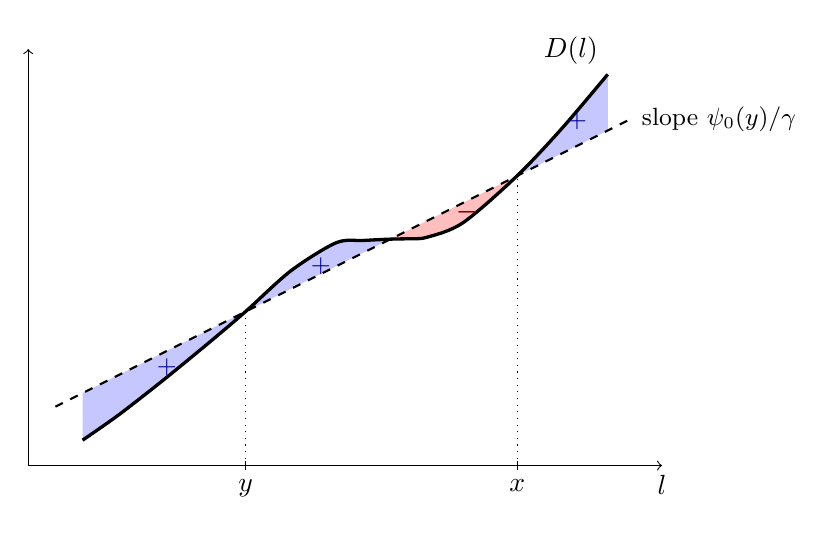
\begin{tikzpicture}[scale=1.15]
\fill[blue!22]
  (0,1.70)
  plot[smooth] coordinates {
    (0,1.70) (-0.4,1.36) (-0.9,0.95) (-1.4,0.56) (-1.8,0.28)
  }
  -- (-1.8,0.80) -- cycle;
\fill[blue!22]
  (0,1.70)
  plot[smooth] coordinates {
    (0,1.70) (0.5,2.15) (1.0,2.46) (1.3,2.485) (1.6,2.50)
  }
  -- cycle;
\fill[red!25]
  (1.6,2.50)
  plot[smooth] coordinates {
    (1.6,2.50) (1.8,2.505) (2.0,2.52) (2.4,2.68) (3.0,3.20)
  }
  -- cycle;
\fill[blue!22]
  (3.0,3.20)
  plot[smooth] coordinates {
    (3.0,3.20) (3.5,3.73) (4.0,4.32)
  }
  -- (4.0,3.70) -- cycle;

\draw[dashed,thick] (-2.1,0.65) -- (4.25,3.825);
\draw[very thick]
  plot[smooth] coordinates {
    (-1.8,0.28) (-1.4,0.56) (-0.9,0.95) (-0.4,1.36)
    (0,1.70) (0.5,2.15) (1.0,2.46) (1.3,2.485)
    (1.6,2.50) (1.8,2.505) (2.0,2.52) (2.4,2.68)
    (3.0,3.20) (3.5,3.73) (4.0,4.32)
  };

\draw[->] (-2.4,0) -- (4.6,0) node[below] {\(l\)};
\draw[->] (-2.4,0) -- (-2.4,4.6);

\draw (0,0.05) -- (0,-0.05) node[below] {\(y\)};
\draw[dotted] (0,0) -- (0,1.70);
\draw (3.0,0.05) -- (3.0,-0.05) node[below] {\(x\)};
\draw[dotted] (3.0,0) -- (3.0,3.20);

\node[above left] at (4.0,4.32) {\(D(l)\)};
\node[right,font=\small] at (4.27,3.825) {
  slope \(\psi_0(y)/\gamma\)
};
\node[blue!55!black,font=\small] at (0.83,2.20) {\(+\)};
\node[red!55!black,font=\small] at (2.45,2.80) {\(\boldsymbol{-}\)};
\node[blue!55!black,font=\small] at (-0.87,1.08) {\(+\)};
\node[blue!55!black,font=\small] at (3.66,3.80) {\(+\)};
\end{tikzpicture}
\caption{The date-zero conditions. The solid curve is the marginal rent \(D\);
the dashed line through \(D(y)\) has slope \(\psi_0(y)/\gamma\).
The local condition requires this slope not to exceed the slope of
\(D\) at \(y\) (at a kink, the minimum of the one-sided slopes). The
global condition requires the signed area between the marginal rent and the
line, from \(y\) to every possible true type \(x\), to be nonnegative.
Blue regions contribute positively to the integral and red regions
negatively.}
\label{fig:timezero}
\end{figure}


The principal internalizes that reducing the slope of $D$ (for example, to iron the allocation to reduce date-zero information rents) lowers the maximum initial marginal rent
volatility and hence limits her ability to expose expected discounted
future allocations to type innovations.


\subsection{Optimal control}\label{sub:control}

The sufficient finite-variation conditions and the necessary local
conditions lead to two control programs. Each program first optimizes
the continuation from a given report, marginal rent, and volatility,
then chooses the date-zero schedules. Under the verification conditions
below, the programs give lower and upper bounds on the principal's
payoff, respectively.

\paragraph{Eliminating transfers.}
Fix a base type \(c\in\Theta\), let \(U_c:=U(c)\), and, for
\(\theta\in\operatorname{int}\Theta\), define
\[
  h_c(\theta)
  :=
  \frac{\mathbbm 1\{\theta\geq c\}-F(\theta)}{f(\theta)},
\]
which generalizes the inverse hazard rate and reduces to \((1-F)/f\)
when \(c\) is the lowest type. Its values at finite endpoints are
immaterial. Substituting the expected transfer from
Proposition~\ref{prop:transfers}\textnormal{(ii)} into the principal's
objective and integrating over initial types gives
\begin{equation}\label{eq:revenue}
  \Pi
  =
  \E\int_0^\infty e^{-rt}
    \bigl[\theta_tX_t-C(X_t)\bigr]\,\dd t
  -\E\bigl[h_c(\theta_0)D(\theta_0)\bigr]
  -U_c,
\end{equation}
and the envelope formula makes individual rationality equivalent to
\begin{equation}\label{eq:ir}
  U_c+\int_c^\theta D(l)\,\dd l
  \geq0
  \qquad\forall\theta\in\Theta.
\end{equation}
The principal's payoff is surplus minus date-zero information rents.

For fixed date-zero schedules, the rent terms in \eqref{eq:revenue}
are constant, so the continuation problem maximizes surplus,
\[
  \E_t\int_t^\infty e^{-r(s-t)}
    \bigl[\hth_sX_s-C(X_s)\bigr]\,\dd s,
\]
subject to delivering the promised marginal rent and volatility.
Continuation utility is \emph{not} a state variable:
Proposition~\ref{prop:transfers} shows that transfers can always be constructed to deliver the correct first-order incentives.

\paragraph{States and controls.}
The continuation state is \((\hth,D,\psi)\). Along the report, the
marginal rent and volatility satisfy
\begin{align}
  \dd D_t
  &=
  \bigl[(r+\lambda)D_t-X_t\bigr]\dd t
  +\psi_{t}\,\dd\hB_t,
  \label{eq:promise-dynamics}\\
  \dd\psi_t
  &=
  \rho\psi_t\,\dd t
  +v_t\,\dd\hB_t
  -\dd K_t,
  \qquad
  \psi_t\geq0.
  \label{eq:volatility-control}
\end{align}
The allocation \(X\) controls the drift of \(D\); \(v\) is the diffusion
coefficient of \(\psi\); and \(K\) lowers \(\psi\). The processes \(v\)
and \(K\) are predictable, and \(K\) is c\`adl\`ag and nondecreasing
with \(K_0=0\); write \(K^c\) for its continuous part.
% CHECK (Sep 2, Claude): predictable vs adapted for K --- the July draft
% required K adapted cadlag; verify which the verification proof needs.
The second equation is the semimartingale form of the requirement that
\(e^{-\rho t}\psi_t\) be a nonnegative supermartingale
(Theorem~\ref{thm:after}). The local program permits a choice of \(v\); the
finite-variation program sets \(v=0\). Once \(\psi\) reaches zero it
remains there---a nonnegative supermartingale is absorbed at
zero---so \(v=0\) and \(K\) is constant thereafter.

These dynamics prevent the principal from resetting \(\psi\) freely
at each date.

\paragraph{The variational inequality.}
For an interior state
\((\hth,D,\psi)\in\mathbb R^2\times(0,\infty)\), let
\(V(\hth,D,\psi)\) be a candidate continuation value. For an allocation
\(x\in\mathcal X\) and a diffusion coefficient \(v\), let
\(\mathcal L^{x,v}\) denote the generator of the states when \(K\) is
constant (i.e., the supermartingale constraint is binding):
\begin{equation}\label{eq:generator}
\begin{aligned}
  \mathcal L^{x,v}V
  :={}&
  \lambda(\overline\theta-\hth)V_{\hth}
  +\bigl[(r+\lambda)D-x\bigr]V_D
  +\rho\psi V_\psi\\
  &+\frac{\gamma^2}{2}V_{\hth\hth}
  +\gamma\psi V_{\hth D}
  +\frac{\psi^2}{2}V_{DD}+\frac{v^2}{2}V_{\psi\psi}
  +v\bigl(
    \gamma V_{\hth\psi}
    +\psi V_{D\psi}
  \bigr).
\end{aligned}
\end{equation}
The two continuation problems differ only in the controls available for
the volatility. Write \(P\in\{\mathrm{FV},\mathrm{loc}\}\) for the
program, and let
\[
  \mathcal A_{\mathrm{FV}}:=\mathcal X\times\{0\},
  \qquad
  \mathcal A_{\mathrm{loc}}:=\mathcal X\times\mathbb R
\]
be the corresponding sets of controls \((x,v)\). Both programs are
governed by the variational inequality
\begin{equation}\label{eq:hjb}
  \min\bigl\{\mathfrak B_P[V],\,V_\psi\bigr\}=0
  \qquad\text{on }\mathbb R^2\times(0,\infty),
\end{equation}
where
\[
  \mathfrak B_P[V]
  :=
  rV-\sup_{(x,v)\in\mathcal A_P}
  \bigl[\hth x-C(x)+\mathcal L^{x,v}V\bigr].
\]
\begin{comment}
In the local program, the supremum over \(v\) is finite only where
\(V_{\psi\psi}<0\), or where \(V_{\psi\psi}=0\) and
\(\gamma V_{\hth\psi}+\psi V_{D\psi}=0\). At \(\psi=0\), both programs use the boundary
condition \eqref{eq:hjb-boundary} of Appendix~\ref{app:verification},
which applies the generator to the restriction of \(V\) to the
boundary where $\psi=0$.
\end{comment}
Intuitively, since the designer can always lower volatility,
\(V_\psi\geq0\). Where \(V_\psi>0\), \(K\) remains constant, the
drift of \(\psi\) is \(\rho\psi\), and the Bellman equation binds: $\mathfrak B_P[V]=0$.
Where \(V_\psi=0\), an infinitesimal reduction has no first-order
value cost, and the Bellman inequality $\mathfrak B_P[V]\geq 0$ may be strict.

\paragraph{The date-zero programs.}
It remains to choose the date-zero schedules. Let \(V^P\) denote a
candidate value for program \(P\). In both programs, \(D\) and \(\psi_0\) are such that the
objective below is well defined. The date-zero program
is
\begin{equation}\label{eq:program}
  \Pi_P
  :=
  \sup_{D(\cdot),\,\psi_0(\cdot),\,U_c}
  \int_\Theta
  \bigl[V^{P}\bigl(\theta,D(\theta),\psi_0(\theta)\bigr)
  -h_c(\theta)D(\theta)\bigr]\,\dd F(\theta)
  \;-\;U_c,
\end{equation}
subject to individual rationality \eqref{eq:ir} and the date-zero
incentive constraints of the program:
\begin{itemize}
  \item[\(\mathrm{FV}\):] \(\psi_0\geq0\) and the integral condition
  \eqref{eq:claim2};
  \item[\(\mathrm{loc}\):] \(D\) has a nondecreasing representative on
  \(\operatorname{int}\Theta\), with derivative \(D'\), and
  \(0\leq\psi_0\leq\gamma D'\) \(F\)-almost everywhere.\footnote{Lemma~\ref{lem:monotone-rents} in the online appendix
shows that \(D\) is nondecreasing in any incentive-compatible
mechanism. If \(D\) is absolutely continuous, monotonicity
follows directly from the derivative bound.}
\end{itemize}
When \(V^P\) is the true continuation value, both date-zero programs are convex:
their feasible sets are convex, and their objectives are concave in the
delivered schedules.\footnote{The state dynamics
are linear, the allocation set is convex, and the flow surplus
\(\theta x-C(x)\) is concave in \(x\). Mixing two feasible mechanisms
therefore delivers the mixed marginal rent and volatility and at least
the corresponding mixture of surplus.}

\paragraph{From a candidate value to a mechanism.}
Given a solution of the variational inequality, construct a candidate optimal mechanism as follows.
\begin{enumerate}
\item Solve the date-zero program for initial promised marginal rent and volatility schedules. 
\item Choose measurable feedback controls
\((x,v)\in\mathcal A_P\) that attain the supremum in
\eqref{eq:hjb}. From each initial state, the resulting
path must satisfy the Bellman equality
\(\mathfrak B_P[V]=0\) at almost every time with \(\psi>0\).
\item Increase \(K^c\) only where \(V_\psi=0\). When possible, raise \(K\) through a jump to lower \(\psi\) to the lowest level that leaves
\(V(\hth,D,\psi)\) unchanged.
\item At \(\psi=0\), set \(v=0\), keep \(K\) constant, and
choose the allocation to satisfy the Bellman equality
\eqref{eq:verification-bellman} at the boundary
(see Appendix~\ref{app:verification}).
\end{enumerate}
Because \(K_0=0\), the initial state must satisfy these requirements
without an initial jump. The verification theorem also requires an
admissible solution of the state equations and delivery of the promised
marginal rent. Appendix~\ref{app:verification} states the martingale,
transversality, and attainment conditions.

\begin{theorem}[Verification]\label{thm:control}
Fix a program \(P\in\{\mathrm{FV},\mathrm{loc}\}\) and write
\(V=V^P\). Let \(M^*=(X^*,T^*)\) be an admissible mechanism,
with initial marginal-rent schedule \(D^*\), initial volatility
schedule \(\psi_0^*\), and utility \(U_c^*\) for the base type \(c\).
Suppose Condition~\ref{cond:verification} holds and:
\begin{enumerate}[beginpenalty=10000]

\item[\textnormal{(i)}]
\(V\) solves \eqref{eq:hjb} for program \(P\), together with
the boundary condition \eqref{eq:hjb-boundary};

\item[\textnormal{(ii)}]
for every initial type \(\theta\in\Theta\), the continuation
of \(M^*\) from \((\theta,D^*(\theta),\psi_0^*(\theta))\)
satisfies \eqref{eq:promise-dynamics}--\eqref{eq:volatility-control}
and the state and control restrictions for \(P\) (stated under
``States and controls'' in Section~\ref{sub:control}).
It satisfies the Bellman equality \eqref{eq:verification-bellman},
and reductions through \(K\) leave \(V\) unchanged as in
\eqref{eq:verification-adjustment};

\item[\textnormal{(iii)}]
\((D^*,\psi_0^*,U_c^*)\) maximizes the date-zero program
\eqref{eq:program}; if \(P=\mathrm{loc}\), \(D^*\) is absolutely
continuous, the derivatives required by \eqref{eq:local-zero}
exist, and \((D^*,\psi_0^*)\) satisfies that condition at every type;

\item[\textnormal{(iv)}]
the transfers of \(M^*\) satisfy
Proposition~\ref{prop:transfers}\textnormal{(i)--(ii)}.

\end{enumerate}
Then \(M^*\) is individually rational and attains \(\Pi_P\).
If \(P=\mathrm{FV}\), it is globally incentive compatible and
optimal among admissible, incentive-compatible, individually
rational finite-variation mechanisms satisfying \eqref{eq:claim2}.
If \(P=\mathrm{loc}\), it is locally incentive compatible and
optimal among admissible locally incentive-compatible,
individually rational mechanisms with an absolutely continuous
initial marginal rent.
\end{theorem}
\begin{corollary}[The bracket]\label{cor:bracket}
Under the conditions of Theorem~\ref{thm:control} for both programs,
\[
  \Pi_{\mathrm{FV}}
  \;\leq\;
  \sup_M\Pi(M)
  \;\leq\;
  \Pi_{\mathrm{loc}},
\]
where the supremum is over admissible, incentive-compatible,
individually rational mechanisms.
\end{corollary}
Proofs are in Online Appendix \ref{app:supp-main-results}.
% NOTE (Sep 2, Claude): corollary assembled from the bound halves of the
% July theorems (thm:control-fv: "implementable lower bound";
% thm:control-loc: "every IC, IR mechanism is feasible for this
% relaxation"). Verify the statement and wire its proof when the control
% appendix is ported.


%Under the verification and attainment hypotheses, if a local-program
%optimizer has finite-variation volatility and satisfies
%\eqref{eq:claim2}, it is feasible for both programs. The two bounds then
%coincide, and the mechanism is optimal.

\section{Application: Financial Market Design}\label{sec:application}


I apply the machinery to a benchmark problem in market
microstructure: a dealer extracts revenue from a trader
whose hedging needs are private and persistent, a dynamic
version of the dealer's problem in
\cite{glosten1989insider}.\footnote{For simplicity, I assume the asset pays no cash flow though the analysis extends straightforwardly if there is no asymmetric information between the dealer and trader on this dimension.
\citet{glosten1989insider} allows for private information
about the asset's payoff.} The first-order approach
fails because the trader may be either a buyer or a seller, creating
countervailing incentives in the sense of
\citet{lewis1989countervailing}: his date-zero incentive constraints can
bind in either direction. I then characterize the solutions to the finite-variation and local programs, discuss their dynamic properties, including the pattern of binding incentive constraints, and show in examples, that the programs yield nearly tight bounds. I then extend the analysis to an exchange
with many traders and market clearing.%, connecting the analysis
%to a broad class of models in market microstructure \citep[e.g.,][]{du2017optimal,malamud2017decentralized,
%chen2021fragmentation,antill2021augmenting}.

\begin{comment}
A monopolistic dealer designs trades and payments for a trader whose
privately observed ideal position is persistent. This is a dynamic
version of the dealer problem in \citet{glosten1989insider}. The trader
may buy or sell, so constraints from upward and downward misreports can
both bind---countervailing incentives in the sense of
\citet{lewis1989countervailing}. They invalidate the first-order
approach for the regular distributions studied below and can generate a
no-trade interval in static dealer models. For uniform and Gaussian
types below, both program solutions instead assign a nonzero initial
trade to every nonzero type.

I compare the first-order relaxation, the finite-variation and local
programs, and the optimal static mechanism, which fixes the allocation
path at date zero. In the examples, the finite-variation mechanism
earns within two percent of the local upper bound, while the static
mechanism earns less than a third as much.
Section~\ref{sub:app-exchange} extends the analysis to an exchange
with many traders and market clearing.
\end{comment}

\subsection{The dealer's problem}\label{sub:app-market}
A dealer trades an asset with a trader whose ideal position evolves
according to
\[
  \dd\theta_t=-\lambda\theta_t\,\dd t+\dd B_t,
  \qquad
  \theta_0\sim F,
\]
where \(\lambda\geq0\) is the mean-reversion rate and the volatility is
normalized to one. Throughout, \(F\) has finite variance and admits a
continuous density \(f\) that is symmetric about zero and positive on
the interior of its support.\footnote{The analysis extends to the case of a nonzero mean by recentering variables.}

The trader's flow payoff from position \(X_t\) and payment \(T_t\) is
\[
  -\frac12(X_t-\theta_t)^2-T_t;
\]
the quadratic term penalizes deviations from the trader's ideal
position, and the asset pays no cash flow. A trader who does not participate holds
\(X_t=0\) and pays nothing. Relative to this outside option, his flow
gain from participation, gross of transfers, is
\[
  u(\theta_t,X_t)
  =
  -\frac12(X_t-\theta_t)^2+\frac12\theta_t^2
  =
  \theta_tX_t-\frac12X_t^2.
\]
Setting \(\widetilde T_t:=T_t+X_t^2/2\) therefore gives the trader the
bilinear flow payoff \(\theta_tX_t-\widetilde T_t\) and the dealer the
flow revenue \(\widetilde T_t-X_t^2/2\): this is the benchmark model
with allocation cost \(C(X)=X^2/2\). The dealer commits to allocation
and transfer rules adapted to the trader's reports and maximizes
expected discounted revenue, subject to incentive compatibility and
individual rationality. Throughout this application, \(T\) continues
to denote the trader's actual payment; \(\widetilde T\) is used only to
apply the benchmark formulas.

Apply the revenue formula \eqref{eq:revenue} using \(\widetilde T\),
base type \(c=0\), and base value \(u_0:=U(0)\). For nonzero types in
the interior of the support, write
\[
  \Lambda(\theta)
  :=
  h_0(\theta)
  =
  \begin{cases}
    \ \ \bigl(1-F(\theta)\bigr)/f(\theta), & \theta>0,\\[2pt]
    -\,F(\theta)/f(\theta), & \theta<0,
\end{cases}
\]
the \emph{two-sided inverse-hazard weight}. The Myerson virtual value of a trader of initial type $\theta$ is $\theta - \Lambda(\theta)$. Buyers' marginal rents
are weighted by the upper tail of \(F\), and sellers' by the lower tail.
The upward jump of \(1/f(0)\) at zero is the source of countervailing
incentives below. Under truthful reporting, the marginal rent
process is \eqref{eq:rent-process}, and the envelope formula
\eqref{eq:envelope} gives
\(U(\theta)=u_0+\int_0^\theta D(l)\,\dd l\).
Since
\(\theta_tX_t-\frac12X_t^2=\frac12\theta_t^2-\frac12(X_t-\theta_t)^2\),
the objective \eqref{eq:revenue} becomes
\begin{multline}\label{eq:app-tracking-revenue}
  \Pi
  =
  \E\left[\int_0^\infty e^{-rt}\frac12\theta_t^2\,\dd t\right]
  -\frac12\E\left[\int_0^\infty
    e^{-rt}(X_t-\theta_t)^2\,\dd t\right]
  \\-\E\bigl[\Lambda(\theta_0)D(\theta_0)\bigr]
  -u_0.
\end{multline}
The first term is first-best surplus and is independent of the mechanism.
The second is the loss from deviations from the trader's ideal
position. The final two terms subtract expected information rents,
\(\mathbb{E}\left[U(\theta_0)\right]=\E[\Lambda(\theta_0)D(\theta_0)]+u_0\). The
dealer thus trades off tracking the ideal position, which requires a minimal level of volatility $\psi$, against reducing
information rents.

At date zero, implementability is checked by comparing the
marginal-rent schedule with its initial volatility. With \(\gamma=1\),
the continuation and integral conditions give the report-by-report
restriction
\begin{equation}\label{eq:app-datezero}
  0\leq\psi_0(y)
  \leq
  \psi_0^{\max}(y)
  :=
  \inf_{m\in\Theta\setminus\{y\}}
  \frac{2}{(m-y)^2}
  \int_{y}^{m}
  \bigl[D(l)-D(y)\bigr]\dd l .
\end{equation}
The upper bound is equivalent to \eqref{eq:claim2}. With
finite-variation continuations it is sufficient for date-zero
incentives; under the regularity in Remark~\ref{rem:necessity}, it is
also necessary.

\subsection{The first-order approach}\label{sub:app-foa}
Here, I adopt the first-order approach and show that it fails.
The first-order approach maximizes \eqref{eq:app-tracking-revenue}
subject only to the envelope formula and participation,
\(U(\theta)\geq0\), ignoring the remaining incentive conditions.

Recall \(\rho=r+2\lambda\). On the positive interior of the support,
define the buyer-side virtual value by
\[
  \theta-\frac{1-F(\theta)}{f(\theta)}
\]
Call \(F\) \emph{regular} if this virtual value is nondecreasing and
positive somewhere, so that \(x^\star\) below is interior. By symmetry,
the seller side then has the same property. Log-concavity of \(f\) is
sufficient. Let
\[
  x^\star
  :=
  \sup\left\{
    \theta\in\operatorname{int}\Theta\cap[0,\infty):
    \theta-\frac{1-F(\theta)}{f(\theta)}\leq0
  \right\}.
\]

\begin{prop}[The first-order relaxation]\label{prop:app-foa}
Suppose \(F\) is regular. The optimal initial marginal rent is
\begin{equation}\label{eq:app-foa}
  D^{\mathrm{FOA}}(\theta)
  =
  \begin{cases}
    \dfrac{\theta-\Lambda(\theta)}{\rho},
      & |\theta|>x^\star,\\[8pt]
    0, & |\theta|\leq x^\star.
  \end{cases}
\end{equation}
Participation binds precisely for
\(\theta\in[-x^\star,x^\star]\). The corresponding allocation is
\begin{equation}\label{eq:app-foa-X}
  X_t^{\mathrm{FOA}}
  =
  \begin{cases}
    \theta_t-\Lambda(\theta_0)e^{-\lambda t},
      & |\theta_0|>x^\star,\\[4pt]
    \theta_t-\theta_0e^{-\lambda t},
      & |\theta_0|\leq x^\star.
  \end{cases}
\end{equation}
Under truthful reporting, \(D_t=X_t^{\mathrm{FOA}}/\rho\), so
\(\psi_t\equiv1/\rho\). The relaxed value of the objective is
\begin{equation}\label{eq:app-foa-value}
  \Pi^{\mathrm{FOA}}
  =
  \frac{1}{2r\rho}
  +\frac{\rho}{2}
    \E\!\left[D^{\mathrm{FOA}}(\theta_0)^2\right].
\end{equation}
The marginal rent is unique up to \(F\)-null sets and the allocation up to
\(\dd t\otimes\dd\mathbb P\)-null sets.
\end{prop}

The proof in Online Appendix~\ref{app:proof-application} uses standard
Lagrangian methods for static mechanism design with type-dependent outside options
\citep{jullien2000participation}. Regularity ensures
\(D^{\mathrm{FOA}}\) nondecreasing. As I soon explain, the first-order solution therefore
fails because it violates the \emph{dynamic} integral condition, not ordinary
monotonicity (which is a requirement from static mechanism design). This failure occurs even under a monotone hazard rate.

Figure~\ref{fig:app-foa} illustrates the solution for
\(F\) uniform on \([-1,1]\).
% Paste this entire figure in place of the original fig:app-foa.
% Uses the manuscript's existing tikz package; no new packages are needed.
% Designed for a 12pt article with 1.5in margins (5.5in text width).
\begin{figure}[htbp]
\centering
\begin{minipage}[t]{0.48\linewidth}
\centering
\vspace{0pt}
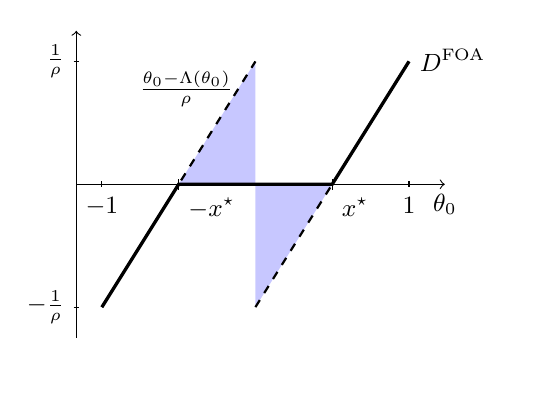
\begin{tikzpicture}[x=0.65cm,y=0.78cm]
% Coordinate scaling leaves all labels at their original font size.
\path[use as bounding box] (-4.45,-2.95) rectangle (4.95,2.55);
% ---- panel (a): first-order rent (uniform) ----
\fill[blue!22] (0,0) -- (-1.5,0) -- (0,2) -- cycle;
\fill[blue!22] (0,0) -- (1.5,0) -- (0,-2) -- cycle;
\draw[dashed,thick] (-3,-2) -- (0,2);
\draw[dashed,thick] (0,-2) -- (3,2);
\draw[very thick] (-3,-2) -- (-1.5,0) -- (1.5,0) -- (3,2);
\draw[->] (-3.5,0) -- (3.7,0) node[below,font=\small] {$\theta_0$};
\draw[->] (-3.5,-2.5) -- (-3.5,2.5);
\draw (-1.5,0.08) -- (-1.5,-0.1);
\node[below right,font=\small] at (-1.5,-0.06) {$-x^\star$};
\draw (1.5,0.08) -- (1.5,-0.1);
\node[below right,font=\small] at (1.5,-0.06) {$x^\star$};
\draw (-3,0.05) -- (-3,-0.05) node[below,font=\small] {$-1$};
\draw (3,0.05) -- (3,-0.05) node[below,font=\small] {$1$};
\draw (-3.55,2) -- (-3.45,2);
\node[left,font=\small] at (-3.55,2) {$\tfrac{1}{\rho}$};
\draw (-3.55,-2) -- (-3.45,-2);
\node[left,font=\small] at (-3.55,-2) {$-\tfrac{1}{\rho}$};
\node[right,font=\small] at (3.02,2.02) {$D^{\mathrm{FOA}}$};
\node[left,font=\small] at (-0.25,1.55)
  {$\tfrac{\theta_0-\Lambda(\theta_0)}{\rho}$};

\end{tikzpicture}
\par\smallskip
{\small (a) the first-order marginal rent\par}
\end{minipage}\hfill
\begin{minipage}[t]{0.48\linewidth}
\centering
\vspace{0pt}
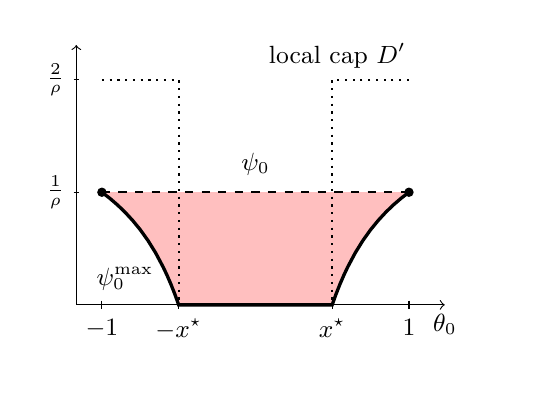
\begin{tikzpicture}[x=0.65cm,y=1.10cm]
\path[use as bounding box] (-4.45,-0.70) rectangle (4.95,3.20);
% ---- panel (b): date-zero condition (uniform) ----
\fill[red!25]
  (-3,1.3) -- (-2.85,1.232) -- (-2.7,1.156) -- (-2.55,1.071)
  -- (-2.4,0.975) -- (-2.25,0.867) -- (-2.1,0.743) -- (-1.95,0.6)
  -- (-1.8,0.433) -- (-1.725,0.339) -- (-1.65,0.236) -- (-1.575,0.124)
  -- (-1.5,0) -- (1.5,0) -- (1.575,0.124) -- (1.65,0.236)
  -- (1.725,0.339) -- (1.8,0.433) -- (1.95,0.6) -- (2.1,0.743)
  -- (2.25,0.867) -- (2.4,0.975) -- (2.55,1.071) -- (2.7,1.156)
  -- (2.85,1.232) -- (3,1.3) -- cycle;
\draw[very thick]
  (-3,1.3) -- (-2.85,1.232) -- (-2.7,1.156) -- (-2.55,1.071)
  -- (-2.4,0.975) -- (-2.25,0.867) -- (-2.1,0.743) -- (-1.95,0.6)
  -- (-1.8,0.433) -- (-1.725,0.339) -- (-1.65,0.236) -- (-1.575,0.124)
  -- (-1.5,0) -- (1.5,0) -- (1.575,0.124) -- (1.65,0.236)
  -- (1.725,0.339) -- (1.8,0.433) -- (1.95,0.6) -- (2.1,0.743)
  -- (2.25,0.867) -- (2.4,0.975) -- (2.55,1.071) -- (2.7,1.156)
  -- (2.85,1.232) -- (3,1.3);
\draw[dashed,thick] (-3,1.3) -- (3,1.3);
\draw[dotted,thick] (-3,2.6) -- (-1.5,2.6) -- (-1.5,0);
\draw[dotted,thick] (3,2.6) -- (1.5,2.6) -- (1.5,0);
\fill (-3,1.3) circle (1.7pt);
\fill (3,1.3) circle (1.7pt);
\draw[->] (-3.5,0) -- (3.7,0) node[below,font=\small] {$\theta_0$};
\draw[->] (-3.5,0) -- (-3.5,3.0);
\draw (-1.5,0.05) -- (-1.5,-0.05)
  node[below,font=\small] {$-x^\star$};
\draw (1.5,0.05) -- (1.5,-0.05)
  node[below,font=\small] {$x^\star$};
\draw (-3,0.05) -- (-3,-0.05) node[below,font=\small] {$-1$};
\draw (3,0.05) -- (3,-0.05) node[below,font=\small] {$1$};
\draw (-3.55,1.3) -- (-3.45,1.3);
\node[left,font=\small] at (-3.55,1.3) {$\tfrac{1}{\rho}$};
\draw (-3.55,2.6) -- (-3.45,2.6);
\node[left,font=\small] at (-3.55,2.6) {$\tfrac{2}{\rho}$};
\node[above,font=\small] at (0,1.38) {$\psi_0$};
\node[font=\small] at (-2.55,0.3) {$\psi_0^{\max}$};
\node[above,font=\small] at (1.60,2.62) {local cap $D'$};

\end{tikzpicture}
\par\smallskip
{\small (b) the date-zero condition\par}
\end{minipage}
\caption{The first-order approach for uniform types. Panel (a) plots
the marginal rent \eqref{eq:app-foa} (solid) and
\((\theta_0-\Lambda(\theta_0))/\rho\) (dashed). Panel (b) compares the
delivered initial marginal rent volatility \(1/\rho\) (dashed), the cap
\(\psi_0^{\max}\) imposed by \eqref{eq:app-datezero} (solid), and the
local cap \(D'\) (dotted). The shading in panel (b) marks the violation
of the cap.}
\label{fig:app-foa}
\end{figure}

Panel~(a) compares \(D^{\mathrm{FOA}}\) (solid) with the virtual value
divided by \(\rho\) (dashed). Holding \(u_0\) fixed, the dealer would
choose the dashed marginal rent schedule if participation constraints were
ignored.\footnote{Without fixing \(u_0\), dropping participation would
allow the dealer to lower every type's utility by the same amount and
obtain unbounded revenue.}
At zero, however, the virtual value jumps downward. Because \(U'=D\),
setting \(u_0=0\) under the dashed schedule would give negative utility
to types immediately on either side of zero. The first-order solution
instead flattens the marginal rent on a central interval:
\[
  D^{\mathrm{FOA}}(\theta_0)=0
  \qquad\text{for }\theta_0\in[-x^\star,x^\star],
\]
where participation constraints bind.

By definition,
\[
  D(\theta_0)
  =
  \E\left[\left.
    \int_0^\infty e^{-(r+\lambda)t}X_t\,\dd t
  \right|\theta_0\right].
\]
Thus central types have zero expected trade discounted at rate
\(r+\lambda\). In fact, for
\(|\theta_0|\leq x^\star\),
\[
  X_t^{\mathrm{FOA}}
  =
  \theta_t-\E[\theta_t\mid\theta_0],
\]
so their expected allocation is zero at every date. At date zero, no
central type trades, as if the dealer charged a bid--ask spread. After date zero, however,
the allocation responds one for one to innovations in the ideal
position. Outside the interval, the dealer partially accommodates the
initial ideal position.

Panel~(b) shows that the first-order solution is not incentive compatible. The solution delivers
initial volatility \(\psi_0=1/\rho\) at every report. Yet, on $[-x^\star,x^\star]$,
the marginal rent is constant, so \(\psi_0^{\max}=0\). In fact, local incentive constraints are violated on this region, since $\psi_0>D'=0$.

Outside the flat $[-x^\star,x^\star]$, local incentive constraints do not bind. The binding incentive constraints are global. For
\(x^\star<|y|<\sup\Theta\), comparing \(y\) with \(-y\) gives
\[
  \psi_0^{\max}(y)
  \leq
  \frac{D^{\mathrm{FOA}}(y)}{y}
  <\frac1\rho.
\]
The integral constraint is therefore violated at \emph{every} interior type.  Because
\(\psi_t\equiv1/\rho\), Remark~\ref{rem:necessity} applies:
violations of the integral constraint correspond to profitable deviations.

\subsection{The finite-variation and local programs}

Because the first-order approach fails, I now turn to the two programs which show how the dealer trades off information rents against responsiveness. I find that the finite-variation solution, at least for the parameter values in
Table~\ref{tab:app-bracket}, is nearly
optimal.

\subsubsection{Continuation values}
\label{sub:app-continuation}

Once the initial marginal rent and volatility are chosen, the dealer
maximizes continuation surplus. In this application, it turns out that the two
programs have the same continuation value, even though the local
program permits a Brownian component in \(\psi\). The quadratic
structure gives a direct solution for the continuation value
which one can verify solves the variational inequality \eqref{eq:hjb} for both programs.

The states follow \eqref{eq:promise-dynamics}--\eqref{eq:volatility-control},
with \(v=0\) in the finite-variation program.

Under the efficient allocation \(X_t=\hth_t\), the marginal rent is
\(\hth_t/\rho\) and its volatility is \(1/\rho\). To measure departures
from these values, define
\[
  \widetilde D_t
  :=
  D_t-\frac{\hth_t}{\rho},
  \qquad
  \zeta_t
  :=
  X_t-\hth_t.
\]
Equation~\eqref{eq:promise-dynamics} then becomes
\[
  \dd\widetilde D_t
  =
  \bigl[(r+\lambda)\widetilde D_t-\zeta_t\bigr]\dd t
  +
  \left(\psi_t-\frac1\rho\right)\dd\hB_t.
\]
Since
\(\hth_tX_t-\frac12X_t^2=\frac12\hth_t^2-\frac12\zeta_t^2\),
maximizing continuation surplus is equivalent to minimizing the
tracking cost: $\E\int_0^\infty e^{-rt}\zeta_t^2\,\dd t$. Applying It\^o's formula to
\(e^{-rt}\rho\widetilde D_t^2/2\), taking expectations, and completing
the square gives
\begin{multline}\label{eq:app-tracking-identity}
  \frac12\E\int_0^\infty e^{-rt}\zeta_t^2\,\dd t
  ={}
  \frac{\rho}{2}\widetilde D_0^2
  +\frac12\E\int_0^\infty e^{-rt}
    \bigl(\zeta_t-\rho\widetilde D_t\bigr)^2\dd t\\
  +\frac{\rho}{2}\E\int_0^\infty e^{-rt}
    \left(\psi_t-\frac1\rho\right)^2\dd t.
\end{multline}

The first term is the cost of the initial promise. The
middle integral vanishes when \(\zeta_t=\rho\widetilde D_t\),
equivalently \(X_t=\rho D_t\). The remaining problem is therefore to
keep \(\psi_t\) as close as possible to its efficient value \(1/\rho\).
Since \(e^{-\rho t}\psi_t\) must be a nonnegative supermartingale,
\(\E[\psi_t]\leq e^{\rho t}\psi_0\), and because the loss is quadratic,
Jensen's inequality gives
\[
  \E\left[
    \left(\psi_t-\frac1\rho\right)^2
  \right]
  \geq
  \left[
    \left(\frac1\rho-e^{\rho t}\psi_0\right)^+
  \right]^2,
\]
the bound being trivial once \(e^{\rho t}\psi_0\geq1/\rho\). For
\(\psi_0\leq1/\rho\), equality holds at every date along the
deterministic finite-variation path
\(\psi_t=\min\{e^{\rho t}\psi_0,\,1/\rho\}\), which is therefore
optimal even among diffusive volatilities.

\begin{prop}[Continuation value]\label{prop:app-fv}
From every initial state
\((\hth,D,\psi)\in\mathbb R^2\times[0,\infty)\), the finite-variation
and local continuation problems have the same value:
\begin{equation}\label{eq:app-value}
  V(\hth,D,\psi)
  =
  \frac{\hth^2}{2\rho}
  +\frac{1}{2r\rho}
  -\frac{\rho}{2}
    \left(D-\frac{\hth}{\rho}\right)^2
  -\frac{\rho}{2}P(\psi),
\end{equation}
where
\[
  P(\psi)
  :=
  \int_0^\infty e^{-rs}
  \left[
    \left(\frac1\rho-e^{\rho s}\psi\right)^+
  \right]^2\dd s.
\]

If \(0\leq\psi\leq1/\rho\), the value is attained in both programs by
\[
  X_t=\rho D_t,
  \qquad
  \psi_t
  =
  \min\left\{e^{\rho t}\psi,\frac1\rho\right\},
  \qquad
  v_t=0.
\]
If \(\psi>1/\rho\), the value in \eqref{eq:app-value} is not attained
but is approached arbitrarily closely by lowering \(\psi\) to
\(1/\rho\) over a shrinking period of time.
\end{prop}

Since \(P\) vanishes at and above \(1/\rho\), raising the initial
volatility past \(1/\rho\) leaves continuation value unchanged and only
tightens the date-zero incentive constraints. Both date-zero programs
may therefore restrict \(\psi_0\leq1/\rho\) without loss.

Under \(X_t=\rho D_t\), the allocation responds to an innovation in the
trader's type with coefficient \(\rho\psi_t\); efficiency requires this
coefficient to equal one, which explains the target \(\psi_t=1/\rho\).
When \(0<\psi_0<1/\rho\), the optimal path raises \(\psi\) at the
fastest rate incentives permit until it reaches \(1/\rho\), and keeps
it there. The dealer's central tradeoff is that lower initial volatility weakens the response to future
shocks but relaxes the date-zero constraints on the marginal rent
schedule.
% NOTE (Sep 2, Claude): the cubic-cost passage (restored Sep 1 from the
% July draft's eq:app-cubic) was removed per DT instruction; the
% general-lambda closed form of P remains recorded in the application
% appendix per the July 30 note.

\subsubsection{The date-zero programs}\label{sub:app-numerics}

Because the continuation values coincide, both date-zero programs take
the form \eqref{eq:program}, with the common value \(V\) of
Proposition~\ref{prop:app-fv} in place of \(V^{P}\) and pricing weight
\(\Lambda=h_0\). The dealer maximizes over measurable \(D\) and
\(\psi_0\) with \(0\leq\psi_0\leq1/\rho\), and over \(u_0\),
subject to participation: \(u_0+\int_0^\theta D(l)\,\dd l\geq0\) for
every \(\theta\). The finite-variation program additionally imposes the cap
\eqref{eq:app-datezero}; the local program instead imposes only the
local conditions, \(D\) nondecreasing and \(\psi_0\leq D'\) almost
everywhere.

For uniform types, both programs admit analytic solutions.
Proposition~\ref{prop:app-uniform-programs} records their main
properties; Online Appendix~\ref{app:structure-uniform} gives the complete
characterizations and proofs. The numerical Gaussian solutions in
Table~\ref{tab:app-bracket} have the same qualitative features.\footnote{There is an interval around zero on which the marginal rent is affine and
the initial volatility constant; outside this interval, only
constraints comparing \(\theta\) with \(-\theta\) bind. In the local
solution, \(\psi_0=D'\) on an inner interval, while outside it the
marginal rent coincides with the first-order solution and the volatility is
first best.}

\begin{prop}[Uniform types]\label{prop:app-uniform-programs}
Suppose \(F\) is uniform on \([-1,1]\). Both date-zero programs have
unique solutions up to \(F\)-null sets. 

\emph{Finite variation.}
There are \(s\in(0,1/\rho)\) and \(b\in(3/8,3/4)\) such that, for
\(|\theta|\leq b\),
\[
  D^{\mathrm{FV}}(\theta)=s\theta,
  \qquad
  \psi_0^{\mathrm{FV}}(\theta)=s.
\]
For \(b<|\theta|\leq1\), the equality
\[
  \psi_0^{\mathrm{FV}}(\theta)
  =
  \frac{D^{\mathrm{FV}}(\theta)}{\theta}
\]
continues to hold, but the ratio now increases strictly with
\(|\theta|\) from \(s\) to \(1/\rho\).

Moreover, every date-zero constraint \eqref{eq:claim2} between two distinct types in
\([-b,b]\) binds. Outside this interval, only date-zero constraints
between types \(\theta\) and \(-\theta\) bind. Initial volatility is
below its first-best level at every interior type and equals
\(1/\rho\) only at the endpoints.

\emph{Local.}
There is \(a\in(1/2,1)\) such that, for \(|\theta|<a\),
\[
  \psi_0^{\mathrm{loc}}(\theta)
  =
  (D^{\mathrm{loc}})'(\theta)
  <
  \frac1\rho.
\]
For \(a\leq|\theta|\leq1\),
\[
  D^{\mathrm{loc}}(\theta)
  =
  D^{\mathrm{FOA}}(\theta),
  \qquad
  \psi_0^{\mathrm{loc}}(\theta)
  =
  \frac1\rho.
\]
The solution violates
\eqref{eq:app-datezero} at every
\(\theta\in(-1,1)\setminus\{0\}\).
\end{prop}

At \(r=1\) and \(\lambda=0\),
\(
  (s,b,a)=(0.5712,\,0.5249,\,0.7497);
\)
Figure~\ref{fig:app-numerics} plots the two solutions at these
parameter values. I discuss their key properties, formalized in the proposition, and offer intuition for them. 


\begin{figure}[h]
\centering
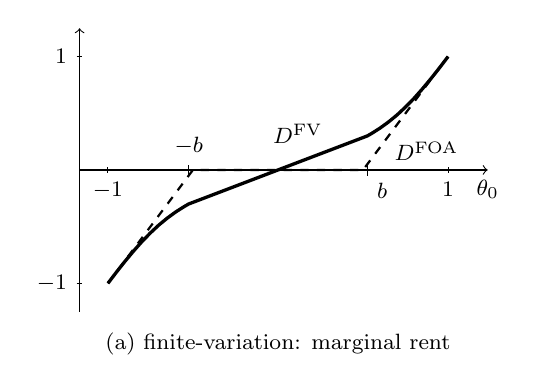
\begin{tikzpicture}[scale=0.72]
% ---- panel (a): finite-variation program, rent ----
\draw[dashed,thick] (-3,-2) -- (-1.5,0) -- (1.5,0) -- (3,2);
\draw[very thick]
  (-3,-2) -- (-2.85,-1.803) -- (-2.7,-1.613) -- (-2.55,-1.433)
  -- (-2.4,-1.264) -- (-2.25,-1.110) -- (-2.1,-0.970) -- (-1.95,-0.847)
  -- (-1.8,-0.738) -- (-1.65,-0.643) -- (-1.575,-0.600)
  -- (1.575,0.600)
  -- (1.65,0.643) -- (1.8,0.738) -- (1.95,0.847) -- (2.1,0.970)
  -- (2.25,1.110) -- (2.4,1.264) -- (2.55,1.433) -- (2.7,1.613)
  -- (2.85,1.803) -- (3,2);
\draw[->] (-3.5,0) -- (3.7,0) node[below,font=\footnotesize] {$\theta_0$};
\draw[->] (-3.5,-2.5) -- (-3.5,2.5);
\draw (-3,0.05) -- (-3,-0.05) node[below,font=\footnotesize] {$-1$};
\draw (3,0.05) -- (3,-0.05) node[below,font=\footnotesize] {$1$};
\draw (-1.575,0.08) -- (-1.575,-0.1);
\node[above,font=\footnotesize] at (-1.575,0.1) {$-b$};
\draw (1.575,0.08) -- (1.575,-0.1);
\node[below right,font=\footnotesize] at (1.575,-0.06) {$b$};
\draw (-3.55,2) -- (-3.45,2); \node[left,font=\footnotesize] at (-3.55,2) {$1$};
\draw (-3.55,-2) -- (-3.45,-2); \node[left,font=\footnotesize] at (-3.55,-2) {$-1$};
\node[above,font=\footnotesize] at (0.35,0.30) {$D^{\mathrm{FV}}$};
\node[font=\footnotesize] at (2.62,0.33) {$D^{\mathrm{FOA}}$};
\node[below,font=\footnotesize] at (0,-2.7) {(a) finite-variation: marginal rent};
\end{tikzpicture}
\hspace{0.55cm}
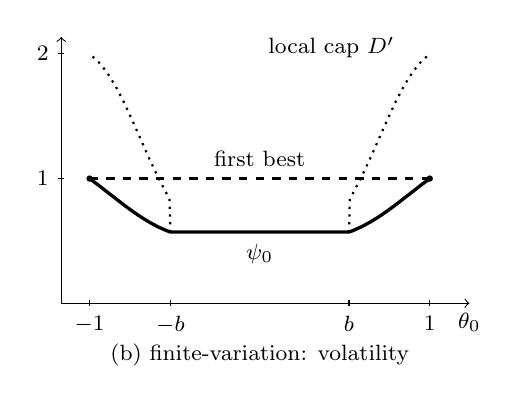
\begin{tikzpicture}[scale=0.72]
% ---- panel (b): finite-variation program, volatility ----
\draw[dashed,thick] (-3,2.2) -- (3,2.2);
\draw[dotted,thick]
  (1.575,1.257) -- (1.59,1.845) -- (1.65,1.950) -- (1.8,2.238)
  -- (1.95,2.557) -- (2.1,2.895) -- (2.25,3.235) -- (2.4,3.557)
  -- (2.55,3.844) -- (2.7,4.082) -- (2.85,4.267) -- (3,4.4);
\draw[dotted,thick]
  (-1.575,1.257) -- (-1.59,1.845) -- (-1.65,1.950) -- (-1.8,2.238)
  -- (-1.95,2.557) -- (-2.1,2.895) -- (-2.25,3.235) -- (-2.4,3.557)
  -- (-2.55,3.844) -- (-2.7,4.082) -- (-2.85,4.267) -- (-3,4.4);
\draw[very thick]
  (-3,2.2) -- (-2.85,2.088) -- (-2.7,1.971) -- (-2.55,1.855)
  -- (-2.4,1.738) -- (-2.25,1.628) -- (-2.1,1.525) -- (-1.95,1.433)
  -- (-1.8,1.352) -- (-1.65,1.284) -- (-1.575,1.257)
  -- (1.575,1.257)
  -- (1.65,1.284) -- (1.8,1.352) -- (1.95,1.433) -- (2.1,1.525)
  -- (2.25,1.628) -- (2.4,1.738) -- (2.55,1.855) -- (2.7,1.971)
  -- (2.85,2.088) -- (3,2.2);
\fill (-3,2.2) circle (1.6pt);
\fill (3,2.2) circle (1.6pt);
\draw[->] (-3.5,0) -- (3.7,0) node[below,font=\footnotesize] {$\theta_0$};
\draw[->] (-3.5,0) -- (-3.5,4.7);
\draw (-3,0.05) -- (-3,-0.05) node[below,font=\footnotesize] {$-1$};
\draw (3,0.05) -- (3,-0.05) node[below,font=\footnotesize] {$1$};
\draw (-3.55,2.2) -- (-3.45,2.2); \node[left,font=\footnotesize] at (-3.55,2.2) {$1$};
\draw (-3.55,4.4) -- (-3.45,4.4); \node[left,font=\footnotesize] at (-3.55,4.4) {$2$};
\draw (-1.575,0.05) -- (-1.575,-0.05) node[below,font=\footnotesize] {$-b$};
\draw (1.575,0.05) -- (1.575,-0.05) node[below,font=\footnotesize] {$b$};
\node[below,font=\footnotesize] at (0,1.21) {$\psi_0$};
\node[above,font=\footnotesize] at (0,2.24) {first best};
\node[above left,font=\footnotesize] at (2.55,4.15) {local cap $D'$};
\node[below,font=\footnotesize] at (0,-0.55) {(b) finite-variation: volatility};
\end{tikzpicture}

\medskip

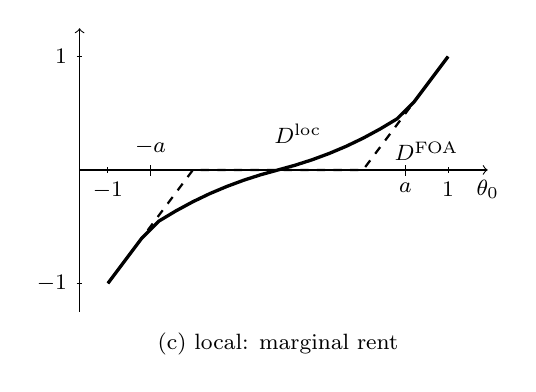
\begin{tikzpicture}[scale=0.72]
% ---- panel (c): local program, rent ----
\draw[dashed,thick] (-3,-2) -- (-1.5,0) -- (1.5,0) -- (3,2);
\draw[very thick]
  (-3,-2) -- (-2.7,-1.6) -- (-2.4,-1.2) -- (-2.1,-0.902)
  -- (-1.8,-0.722) -- (-1.5,-0.560) -- (-1.2,-0.416) -- (-0.9,-0.290)
  -- (-0.6,-0.179) -- (-0.3,-0.083) -- (0,0) -- (0.3,0.083)
  -- (0.6,0.179) -- (0.9,0.290) -- (1.2,0.416) -- (1.5,0.560)
  -- (1.8,0.722) -- (2.1,0.902) -- (2.4,1.2) -- (2.7,1.6) -- (3,2);
\draw[->] (-3.5,0) -- (3.7,0) node[below,font=\footnotesize] {$\theta_0$};
\draw[->] (-3.5,-2.5) -- (-3.5,2.5);
\draw (-3,0.05) -- (-3,-0.05) node[below,font=\footnotesize] {$-1$};
\draw (3,0.05) -- (3,-0.05) node[below,font=\footnotesize] {$1$};
\draw (-3.55,2) -- (-3.45,2); \node[left,font=\footnotesize] at (-3.55,2) {$1$};
\draw (-3.55,-2) -- (-3.45,-2); \node[left,font=\footnotesize] at (-3.55,-2) {$-1$};
\draw (-2.249,0.08) -- (-2.249,-0.1);
\node[above,font=\footnotesize] at (-2.249,0.1) {$-a$};
\draw (2.249,0.08) -- (2.249,-0.1);
\node[below,font=\footnotesize] at (2.249,-0.06) {$a$};
\node[above,font=\footnotesize] at (0.35,0.30) {$D^{\mathrm{loc}}$};
\node[font=\footnotesize] at (2.62,0.33) {$D^{\mathrm{FOA}}$};
\node[below,font=\footnotesize] at (0,-2.7) {(c) local: marginal rent};
\end{tikzpicture}
\hspace{0.55cm}
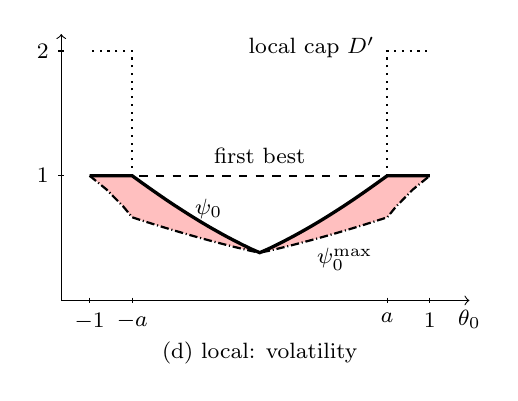
\begin{tikzpicture}[scale=0.72]
% ---- panel (d): local program, volatility ----
\fill[red!25]
  (0,0.843) -- (0.15,0.908) -- (0.3,0.981) -- (0.45,1.057)
  -- (0.6,1.136) -- (0.75,1.219) -- (0.9,1.304) -- (1.05,1.393)
  -- (1.2,1.485) -- (1.35,1.580) -- (1.5,1.677) -- (1.65,1.777)
  -- (1.8,1.880) -- (1.95,1.985) -- (2.1,2.092) -- (2.25,2.2)
  -- (3,2.2) -- (2.7,1.956) -- (2.4,1.65) -- (2.25,1.467)
  -- (2.1,1.418) -- (1.95,1.370) -- (1.8,1.323) -- (1.65,1.277)
  -- (1.5,1.232) -- (1.35,1.188) -- (1.2,1.145) -- (1.05,1.103)
  -- (0.9,1.062) -- (0.75,1.022) -- (0.6,0.983) -- (0.45,0.945)
  -- (0.3,0.909) -- (0.15,0.873) -- cycle;
\fill[red!25]
  (0,0.843) -- (-0.15,0.908) -- (-0.3,0.981) -- (-0.45,1.057)
  -- (-0.6,1.136) -- (-0.75,1.219) -- (-0.9,1.304) -- (-1.05,1.393)
  -- (-1.2,1.485) -- (-1.35,1.580) -- (-1.5,1.677) -- (-1.65,1.777)
  -- (-1.8,1.880) -- (-1.95,1.985) -- (-2.1,2.092) -- (-2.25,2.2)
  -- (-3,2.2) -- (-2.7,1.956) -- (-2.4,1.65) -- (-2.25,1.467)
  -- (-2.1,1.418) -- (-1.95,1.370) -- (-1.8,1.323) -- (-1.65,1.277)
  -- (-1.5,1.232) -- (-1.35,1.188) -- (-1.2,1.145) -- (-1.05,1.103)
  -- (-0.9,1.062) -- (-0.75,1.022) -- (-0.6,0.983) -- (-0.45,0.945)
  -- (-0.3,0.909) -- (-0.15,0.873) -- cycle;
\draw[dashed,thick] (-3,2.2) -- (3,2.2);
\draw[dotted,thick]
  (2.249,2.2) -- (2.249,4.4) -- (3,4.4);
\draw[dotted,thick]
  (-2.249,2.2) -- (-2.249,4.4) -- (-3,4.4);
\draw[densely dashdotted,thick]
  (-3,2.2) -- (-2.7,1.956) -- (-2.4,1.65) -- (-2.25,1.467)
  -- (-2.1,1.418) -- (-1.95,1.370) -- (-1.8,1.323) -- (-1.65,1.277)
  -- (-1.5,1.232) -- (-1.35,1.188) -- (-1.2,1.145) -- (-1.05,1.103)
  -- (-0.9,1.062) -- (-0.75,1.022) -- (-0.6,0.983) -- (-0.45,0.945)
  -- (-0.3,0.909) -- (-0.15,0.873) -- (0,0.843) -- (0.15,0.873)
  -- (0.3,0.909) -- (0.45,0.945) -- (0.6,0.983) -- (0.75,1.022)
  -- (0.9,1.062) -- (1.05,1.103) -- (1.2,1.145) -- (1.35,1.188)
  -- (1.5,1.232) -- (1.65,1.277) -- (1.8,1.323) -- (1.95,1.370)
  -- (2.1,1.418) -- (2.25,1.467) -- (2.4,1.65) -- (2.7,1.956)
  -- (3,2.2);
\draw[very thick]
  (-3,2.2) -- (-2.25,2.2) -- (-2.1,2.092) -- (-1.95,1.985)
  -- (-1.8,1.880) -- (-1.65,1.777) -- (-1.5,1.677) -- (-1.35,1.580)
  -- (-1.2,1.485) -- (-1.05,1.393) -- (-0.9,1.304) -- (-0.75,1.219)
  -- (-0.6,1.136) -- (-0.45,1.057) -- (-0.3,0.981) -- (-0.15,0.908)
  -- (0,0.843) -- (0.15,0.908) -- (0.3,0.981) -- (0.45,1.057)
  -- (0.6,1.136) -- (0.75,1.219) -- (0.9,1.304) -- (1.05,1.393)
  -- (1.2,1.485) -- (1.35,1.580) -- (1.5,1.677) -- (1.65,1.777)
  -- (1.8,1.880) -- (1.95,1.985) -- (2.1,2.092) -- (2.25,2.2)
  -- (3,2.2);
\draw[->] (-3.5,0) -- (3.7,0) node[below,font=\footnotesize] {$\theta_0$};
\draw[->] (-3.5,0) -- (-3.5,4.7);
\draw (-3,0.05) -- (-3,-0.05) node[below,font=\footnotesize] {$-1$};
\draw (3,0.05) -- (3,-0.05) node[below,font=\footnotesize] {$1$};
\draw (-3.55,2.2) -- (-3.45,2.2); \node[left,font=\footnotesize] at (-3.55,2.2) {$1$};
\draw (-3.55,4.4) -- (-3.45,4.4); \node[left,font=\footnotesize] at (-3.55,4.4) {$2$};
\draw (-2.249,0.05) -- (-2.249,-0.05) node[below,font=\footnotesize] {$-a$};
\draw (2.249,0.05) -- (2.249,-0.05) node[below,font=\footnotesize] {$a$};
\node[font=\footnotesize] at (-0.9,1.62) {$\psi_0$};
\node[font=\footnotesize] at (1.5,0.72) {$\psi_0^{\max}$};
\node[above,font=\footnotesize] at (0,2.24) {first best};
\node[above left,font=\footnotesize] at (2.2,4.1) {local cap $D'$};
\node[below,font=\footnotesize] at (0,-0.55) {(d) local: volatility};
\end{tikzpicture}
\caption{Date-zero solutions for uniform types at \(r=1\) and
\(\lambda=0\). Solid curves are the program solutions. In the marginal rent
panels, the dashed curve is the first-order marginal rent. In the volatility
panels, the dashed line is first-best volatility and the dotted curve
is the local cap \(D'\). Panel \textnormal{(d)} also shows the global
cap \(\psi_0^{\max}\) (dash-dotted); the shaded region is the amount
by which the local solution violates that cap.}
\label{fig:app-numerics}
\end{figure}

\begin{comment}
The first-order solution bunches central initial
types: the rent is flat, and expected trade conditional on the initial type
is zero. This is the date-zero analogue of a bid--ask spread. Buyers' and
sellers' rents are priced from opposite tails of \(F\), so the marginal
terms of trade jump when the trader switches from selling to buying, leaving
small initial desired trades unfilled. Traders in the bunching region do trade after $t=0$ since the allocation is exposed to their future type shocks but do not trade initially.
\end{comment}

Neither program retains the first-order solution's central no-trade interval. Thus, bunching is not robust to dynamics. In contrast, under the finite-variation solution, there is a central region$[-b,b]$ where the marginal rent is affine
\[
  D^{\mathrm{FV}}(\theta_0)=s\theta_0,
  \qquad
  X_0^{\mathrm{FV}}=\rho s\theta_0
  \quad\text{for }|\theta_0|\leq b,
\]
so every nonzero central type trades a fraction \(\rho s\in(0,1)\)
of his ideal position. The allocation's response to later type
innovations rises from \(\rho s\) to one as volatility grows at the
maximum permitted rate to \(1/\rho\). In this central region, local incentive constraints bind. 

Outside the central interval, this is not so. For
\(|\theta_0|>b\), the local condition is slack, but the integral constraint \eqref{eq:claim2}
comparing \(\theta_0\) with \(-\theta_0\) binds. Because
the marginal rent is an odd function, this caps the initial volatility at
\(D^{\mathrm{FV}}(\theta_0)/\theta_0\)---the average slope of the marginal rent
between these types---rather than at the local slope. Initial
volatility is therefore below first best at \emph{every} interior type.

In contrast, the local solution is only distorted on  the interval \((-a,a)\). The local solution nevertheless exceeds the cap \(\psi_0^{\max}\)
implied by its own marginal rent at \emph{every} nonzero interior type as seen from the shaded area in panel~(d). Its optimal
continuation has deterministic, absolutely continuous volatility, so
Remark~\ref{rem:necessity} makes the cap necessary. The local-program
solution is therefore not globally incentive compatible.

\begin{comment}
Symmetry and uniqueness make both marginal-rent schedules odd, and
revenue maximization sets \(u_0=0\). Because both schedules are
strictly increasing, participation binds only at \(\theta_0=0\). Thus
no nonzero type is excluded.
\end{comment}

For different values of $\lambda$, 
Table~\ref{tab:app-bracket} reports the gap between the
finite-variation lower bound and the local upper bound for the uniform and Gaussian distributions. It also reports the values under the static benchmark and first-order solution, whose gap captures the value of responding to later reports. (The static
benchmark fixes the entire allocation path as a function of the initial report;
Online Appendix~\ref{app:static-benchmark} shows that its optimal allocation is
\(X_t^{\mathrm{stat}}=\E[X_t^{\mathrm{FOA}}\mid\theta_0]\).) The uniform
entries come from the analytic solutions above; the Gaussian entries
are computed from discretized versions of the programs
(Online Appendix~\ref{app:numerics-details}).

\begin{table}[ht]
\centering
\begin{tabular}{@{}lcccc@{}}
\toprule
& \multicolumn{2}{c}{Uniform on \([-1,1]\)}
& \multicolumn{2}{c}{Gaussian} \\
\cmidrule(lr){2-3}\cmidrule(lr){4-5}
& \(\lambda=0\) & \(\lambda=\tfrac12\)
& \(\lambda=0\) & \(\lambda=\tfrac12\) \\
\midrule
Static
& \(15.3\%\) & \(15.1\%\) & \(32.3\%\) & \(31.6\%\) \\
Finite variation
& \(99.0\%\) & \(99.0\%\) & \(98.2\%\) & \(98.4\%\) \\
Local program
& \(100\%\) & \(100\%\) & \(100\%\) & \(100\%\) \\
First-order approach
& \(107.3\%\) & \(106.0\%\) & \(110.8\%\) & \(108.4\%\) \\
\midrule
\(\Pi_{\mathrm{loc}}\)
& \(0.5435\) & \(0.2752\) & \(0.6375\) & \(0.3258\) \\
\bottomrule
\end{tabular}
\caption{Revenue as a percentage of the local upper bound
\(\Pi_{\mathrm{loc}}\). The final row gives its level; \(r=1\)
throughout, and the Gaussian columns use the standard normal. The finite-variation value is attained by an implementable
mechanism and is a lower bound on unrestricted revenue; the local value
is an upper bound; the first-order row is an infeasible relaxation.
Uniform entries are analytic; Gaussian entries are computed on a grid.}
\label{tab:app-bracket}
\end{table}

For uniform types, the finite-variation mechanism attains \(99.0\%\)
of the local upper bound. The Gaussian computations give gaps of
\(1.6\%\)--\(1.8\%\). The first-order value exceeds the local upper
bound by \(6\)--\(11\) percentage points, so most of its apparent gain
over finite variation is infeasible. By contrast, the static mechanism
earns only \(15\%\)--\(32\%\) of the local value. Responding to later
reports is therefore quantitatively important, and the finite-variation
mechanism captures nearly all of that value in these examples.

\subsection{From dealer to exchange}
\label{sub:app-exchange}
The analysis extends to an exchange with many traders: under the
conditions below, the exchange's problem reduces to one dealer problem
per trader. Consider an exchange that reallocates the asset among \(N\)
traders, each as in Section~\ref{sub:app-market}, with independent
trading needs. Related models with private trading needs and quadratic
costs of deviations from ideal positions typically take the trading
protocol as given
\citep[e.g.,][]{du2017optimal,malamud2017decentralized,
chen2021fragmentation,antill2021augmenting}.\footnote{An exception is
\citet{chen2024optimal}, which studies the static counterpart in which
the exchange chooses the mechanism.} Here the exchange chooses
allocation and transfer rules to maximize total revenue, subject to
incentive compatibility, interim participation, and market clearing at
every date: \(\sum_{i=1}^N X_t^i=0\).

Each trader's reports may depend on the histories of his own types, his
past reports, and the allocations he observes, as in
\citet{pavan2014dynamic}.
Online Appendices~\ref{app:exchange-admissibility}--\ref{app:proof-exchange}
give the precise definitions of admissible exchange reports and
mechanisms and prove the corollary
below.

Three classes of dealer mechanisms are relevant: \(\mathrm G\), the
admissible, globally incentive-compatible, individually rational
mechanisms; \(\mathrm{FV}\), the finite-variation mechanisms feasible
in the finite-variation program---those satisfying the conditions of
Theorems~\ref{thm:after} and~\ref{thm:zero} and the cap
\eqref{eq:app-datezero}; and \(\mathrm L\), the admissible locally
incentive-compatible mechanisms of the local program.

For \(\mathcal C\in\{\mathrm G,\mathrm{FV},\mathrm L\}\), let
\(\mathcal D_{\mathcal C}^i\) denote the admissible, individually rational
dealer mechanisms for trader \(i\) in class \(\mathcal C\), and let
\(\mathcal E_{\mathcal C}\) denote the feasible \(N\)-trader exchange
mechanisms in that class, as defined in
Online Appendix~\ref{app:exchange-admissibility}. Define
\[
  \Pi_{\mathcal C}^{\mathrm{ex}}
  :=
  \sup_{M=\{(X^i,T^i)\}_{i=1}^N\in\mathcal E_{\mathcal C}}
  \sum_{i=1}^N
  \E\int_0^\infty e^{-rt}T_t^i\,\dd t.
\]

\begin{corollary}[Exchange decomposition]\label{cor:app-exchange}
Fix \(\mathcal C\in\{\mathrm G,\mathrm{FV},\mathrm L\}\). Suppose that,
for every trader \(i\), the dealer problem
\[
  \sup_{(X,T)\in\mathcal D_{\mathcal C}^i}
  \E\int_0^\infty e^{-rt}T_t\,\dd t
\]
has a solution, and let \(X_{\mathcal C}^{i\ast}\) denote its optimal
allocation. If \(\mathcal C=\mathrm G\), suppose the solutions satisfy
the integrability condition
\eqref{eq:app-exchange-implementation-integrability} in Online
Appendix~\ref{app:proof-exchange}. Set
\[
  \widehat X_{\mathcal C}^i
  :=
  X_{\mathcal C}^{i\ast}
  -\frac1N\sum_{j=1}^N X_{\mathcal C}^{j\ast}.
\]
Then there exist transfers
\(\{\widehat T_{\mathcal C}^i\}_{i=1}^N\) such that
\[
  \widehat M_{\mathcal C}
  :=
  \bigl\{
    (\widehat X_{\mathcal C}^i,\widehat T_{\mathcal C}^i)
  \bigr\}_{i=1}^N
  \in\mathcal E_{\mathcal C}
\]
and
\[
  \sum_{i=1}^N
  \E\int_0^\infty e^{-rt}\widehat T_{\mathcal C,t}^i\,\dd t
  =
  \Pi_{\mathcal C}^{\mathrm{ex}}.
\]
\end{corollary}

The proof first restricts deviations to reports adapted to a trader's
own type history. A projection argument shows that the mechanisms in
the corollary solve this relaxed problem. The proof then uses additive separability of the allocation in the
other traders' reports to show incentive
compatibility when reports also respond to observed allocations.

\section{Extensions}\label{sec:extensions}

I summarize three extensions analyzed in Online
Appendices~\ref{app:gbm}--\ref{app:beyond-fv}.

\subsection{Geometric Brownian Motion}
\label{sec:gbm}

Online Appendix~\ref{app:gbm} extends the analysis to the case when types follow a geometric
Brownian motion, another canonical specification  likely to arise in applications:
\[
  \dd\theta_t=\mu\theta_t\,\dd t+\gamma\theta_t\,\dd B_t,
  \qquad \theta_0\in\Theta\subseteq(0,\infty),\quad r>\mu.
\]
Reports follow the same dynamics with \(B\) replaced by \(\hB\).
In contrast with the OU case, the impulse response \(I_{s,t}=\theta_s/\theta_t\) is stochastic,
so the marginal information rent is
\begin{equation}\label{eq:gbm-rent}
  D_t=\E_t\!\left[\int_t^\infty e^{-r(s-t)}
    \frac{\theta_s}{\theta_t}X_s\,\dd s\right].
\end{equation}
Write \(\psi_t:=\vol(D_t)\) and
\(A_t:=e^{-rt}\hth_t\psi_t\). The results for the OU case generalize to this setting. The following theorem is the analog of Theorems \ref{thm:after} and \ref{thm:zero} for the GBM case. 

\begin{theorem}[Implementability under GBM]\label{thm:gbm}
Suppose the mechanism satisfies the GBM admissibility conditions of
Online Appendix~\ref{app:gbm}, and transfers satisfy
\(\vol(W_t)=\gamma\hth_tD_t\) and the date-zero envelope condition
\eqref{eq:envelope}.
\begin{enumerate}[label=\textnormal{(\roman*)},beginpenalty=10000]
\item Truthful reporting is locally incentive compatible after the
initial report if and only if \(A\) admits a nonnegative c\`adl\`ag
supermartingale representative under truthful continuation from every
initial report. If this representative has finite variation, local
and global incentive compatibility after the initial report are
equivalent.

\item Suppose the supermartingale condition in \textnormal{(i)} holds.
If \(D\) is differentiable, truthful reporting is locally incentive
compatible if and only if
\begin{equation}\label{eq:gbm-local-zero}
  \psi_0(x)\leq\gamma xD'(x)
  \qquad \forall x\in\Theta.
\end{equation}
If the representative of $A$ has finite variation after every truthful initial report,
truthful reporting is globally incentive compatible whenever
\begin{equation}\label{eq:gbm-global-zero}
  \int_y^x\left[D(l)-D(y)
    -\frac{\psi_0(y)}{\gamma}\frac{l-y}{l}\right]\dd l
  \geq0
  \qquad \forall x,y\in\Theta.
\end{equation}
\end{enumerate}
\end{theorem}

The integral condition is also necessary under the regularity in
Remark~\ref{rem:necessity}, with \(A\) in place of \(\psi\).
The finite-variation restriction here is on \(A\), so \(\psi\) itself
may still have a Brownian component.

\subsection{Contracting without Transfers}
Online Appendix~\ref{app:no-transfers} extends
Theorems~\ref{thm:after} and~\ref{thm:zero} to contracts without
transfers showing that it is relevant even outside the Myersonian setting. Call a contract \emph{first-order} if, under truthful
continuation from every initial report, the agent's continuation value
has the volatility of
Proposition~\ref{prop:transfers}(i).

\begin{prop}[Incentives without transfers]\label{prop:no-transfers}
Suppose that \(T\equiv0\). Under the
maintained admissibility and regularity conditions, the conclusions of
Theorem~\ref{thm:after} apply as stated to every first-order contract. If,
in addition, the contract satisfies the date-zero envelope condition in
Proposition~\ref{prop:transfers}(ii), then the conclusions of
Theorem~\ref{thm:zero} also apply under the hypotheses stated
there.
\end{prop}

Without transfers, however, a recursive formulation generally requires continuation utility as an additional state variable, as in \cite{williams2011persistent} or \cite{bloedel2023persistent}.

\subsection{Beyond Finite Variation}
\label{sub:beyond-fv}


Online Appendix~\ref{app:beyond-fv} uses the master formula in
Lemma~\ref{lem:master} to study global incentive compatibility beyond
finite variation. The purpose of the section is to elucidate why global incentive compatibility is difficult to characterize in a way amenable to optimal control, 
explain why the finite-variation class side-steps this difficulty, and provide
intuition for how to construct classes of contracts that can be easily certified as incentive compatible in applications.


Fix a truthful initial report and
write \(\vol^0(\psi):=\psi\) and
\(\vol^{j+1}(\psi):=\vol(\vol^j(\psi))\).
Repeating the integration by parts in \eqref{eq:second-order}
gives\footnote{This formula assumes each volatility has an It\^{o} representation, terminal terms vanish in the integration by parts,
and the remainder vanishes as the number of integrations grows.}
\begin{multline}\label{eq:cascade}
  U_x(x,a)-U(x)
  =\sum_{k=2}^{\infty}\frac{(-1)^{k-1}}{k!\,\gamma^{k-1}}
    \E_x\!\int_0^\infty e^{-rt}\delta_t^k\\
  \times\Bigl[(r+k\lambda)\vol^{k-2}(\psi_t)
    -\drift\!\bigl(\vol^{k-2}(\psi_t)\bigr)\Bigr]\dd t
\end{multline}
for the gain from an arbitrary deviation. A simple characterization of incentives is thus difficult to obtain because all higher order terms in $\delta$ must be controlled. Finite variation is tractable because it removes every term
with \(k\geq3\) since \(\vol(\psi)=0\). The formula also yields intuition for contracts, beyond the finite-variation case, for which incentive compatiblity is easy to check: contracts such that successive
volatilities follow a simple pattern, so that higher-order terms can be summed. A simple case is when $\psi$ follows a geometric Brownian motion. 

\begin{prop}[Proportional volatility]\label{prop:proportional-volatility}
Let \(M\) be an admissible mechanism with transfers satisfying
Proposition~\ref{prop:transfers}\textnormal{(i)}. Suppose \(\psi\)
admits an It\^o representative satisfying, under truthful continuation
from every initial report,
\[
  \dd\psi_t=m_t\,\dd t+\alpha\psi_t\,\dd B_t,
  \qquad \psi_t\geq0,\quad m_t\leq(r+\lambda)\psi_t,
\]
where \(\alpha\neq0\) is constant. Then truthful reporting is globally
incentive compatible after the initial report.
\end{prop}

Here \(\vol^j(\psi)=\alpha^j\psi\), so \eqref{eq:cascade} sums to
\[
  U_x(x,a)-U(x)
  =\frac{\gamma}{\alpha^2}\E_x\!\int_0^\infty e^{-rt}
    \Bigl[\bigl(m_t-(r+\lambda)\psi_t\bigr)h(z_t)
      -\lambda\psi_t g(z_t)\Bigr]\dd t,
\]
where \(z_t:=\alpha\delta_t/\gamma\),
\(h(z):=e^{-z}-1+z\), and \(g(z):=1-(1+z)e^{-z}\).
Both functions are nonnegative.
The sufficient bound is stronger than the local bound
\(m_t\leq(r+2\lambda)\psi_t\) when \(\lambda>0\); they coincide when
\(\lambda=0\).

%In ongoing work, I am exploring additional classes beyond finite
%variation for which global incentive compatibility can be checked
%directly.


% ALTERNATIVE 7.3: INFORMAL VERSION
% To use this version, replace the active subsection above with this block.
% The subsection and equation labels are intentionally the same.
\begin{comment}
\subsection{Beyond Finite Variation}
\label{sub:beyond-fv}
\begin{samepage}

In the OU model, the master formula in Lemma~\ref{lem:master}
explains why global incentive compatibility is harder to characterize
beyond finite variation. Fix a truthful initial report, and write
\(\vol^0(\psi):=\psi\) and
\(\vol^{j+1}(\psi):=\vol(\vol^j(\psi))\).
Repeating the integration by parts in \eqref{eq:second-order}
gives\footnote{This discussion is informal: assume the successive
It\^o decompositions and integrations are justified, the terminal
terms vanish, and the remainder tends to zero as the number of
integrations grows.
In the example below, retaining the nonpositive terminal contribution
leaves the sufficient condition unchanged.}
\begin{multline}\label{eq:cascade}
  U_x(x,a)-U(x)
  =\sum_{k=2}^{\infty}\frac{(-1)^{k-1}}{k!\,\gamma^{k-1}}
    \E_x\!\int_0^\infty e^{-rt}\delta_t^k\\
  \times\Bigl[(r+k\lambda)\vol^{k-2}(\psi_t)
    -\drift\!\bigl(\vol^{k-2}(\psi_t)\bigr)\Bigr]\dd t.
\end{multline}
This is the cascade of higher-order terms in \(\delta\). The local
drift bound controls only the quadratic term; global incentive
compatibility requires bounding the entire sum for deviations of
arbitrary size. Finite variation removes every term with \(k\geq3\)
because \(\vol(\psi)=0\).

For some contracts beyond finite variation, these terms can be summed
explicitly. For example, suppose an
admissible mechanism satisfying the transfer conditions has
\[
  \dd\psi_t=m_t\,\dd t+\alpha\psi_t\,\dd\hB_t,
  \qquad \psi_t\geq0,\quad \alpha\neq0\text{ constant}.
\]
Here \(\vol^j(\psi)=\alpha^j\psi\), so \eqref{eq:cascade} sums to
\[
  U_x(x,a)-U(x)
  =\frac{\gamma}{\alpha^2}\E_x\!\int_0^\infty e^{-rt}
    \Bigl[\bigl(m_t-(r+\lambda)\psi_t\bigr)h(z_t)
      -\lambda\psi_t g(z_t)\Bigr]\dd t,
\]
where \(z_t:=\alpha\delta_t/\gamma\),
\(h(z):=e^{-z}-1+z\), and \(g(z):=1-(1+z)e^{-z}\).
Both functions are nonnegative, so \(m_t\leq(r+\lambda)\psi_t\)
ensures global incentive compatibility after the initial report,
while allowing a Brownian component in \(\psi\).
This sufficient bound is stronger than the local bound
\(m_t\leq(r+2\lambda)\psi_t\) when \(\lambda>0\); they coincide when
\(\lambda=0\).

In ongoing work, I am exploring additional classes beyond finite
variation for which global incentive compatibility can be checked
directly.
\end{samepage}
\end{comment}
\section{Concluding Discussion}\label{sec:conclusion}

This paper connects Myersonian dynamic mechanism design with the
martingale methods of continuous-time contracting and shows that this connection can yield new insights. The main result
characterizes incentives in terms of the volatility of the agent's
marginal information rent.

Under the usual envelope conditions, truthful reporting after the
initial report is locally incentive compatible if and only if the
discounted volatility is a nonnegative supermartingale. For
finite-variation mechanisms, the same condition characterizes global
incentive compatibility after the initial report. The associated drift
constraint makes the design problem amenable to optimal control with
volatility as a state variable. I present two programs that bracket the designer's
payoff even when the first-order approach fails. I apply them to
a benchmark model of financial market design, where the first-order approach fails due to countervailing
incentives.

Most of the paper carries continuous-time methods into the
Myersonian setting.
The discrete-time Myersonian methods, however, also yield insights for
continuous-time contracting. The integral-monotonicity condition
can be used to conjecture, through elementary algebra, the correct conditions for local
incentive compatibility. It also
reveals finite-variation mechanisms as the counterpart of
discrete-time ``linear mechanisms.'' Further, the paper's characterization of incentives extends to settings without transfers for the first-order contracts of Section~\ref{sec:extensions}. When the agent can distort the drift of his reports in either direction,
the supermartingale condition on marginal rent volatility completes
the characterization of local incentive compatibility.

Several directions remain open. First, the local analysis appears
adaptable to general utility functions. For finite-variation mechanisms,
however, the resulting incentive conditions are likely to remain
sufficient but may no longer be necessary: concavity in type can
introduce slack. A second direction is to consider general Markov
diffusions. The two extensions are closely related:  when
utility is multiplicatively separable in type and allocation, a
redefinition of the type variable maps curvature into a change of
diffusion, in which case the two extensions are isomorphic. 

Finally, the
exchange application shows that the results already speak to multi-agent
settings in which the optimal allocation is additively separable across
agents' reports. Implementability when the volatility of each agent's marginal rent
depends on the others' reports is open to investigation.

% PREVIOUS CONCLUDING DISCUSSION (preserved for restoration)
% To restore, replace the active section above with the section in this block.
\begin{comment}
\section{Concluding Discussion}\label{sec:conclusion}

This paper makes transparent the connection between the methods of dynamic
mechanism design in the Myersonian tradition and the martingale methods of
continuous-time contracting, and shows how this connection can yield new
insights. The main result characterizes incentives in terms of the volatility
of the agent's marginal information rents. 

Following the initial report, and under the usual envelope conditions, a supermartingale restriction on this volatility is necessary and sufficient for local incentive compatibility. Within the class of finite-variation contracts, the same restriction also characterizes global incentive compatibility. Because the condition can be imposed pointwise through a drift constraint on the volatility process, the design problem is amenable to optimal control with volatility as a state variable: I present two
programs that together bracket the designer's payoff even where the first-order approach fails.
The machinery is put to work in a benchmark setting from financial market
microstructure, where that failure occurs for fundamental economic reasons.


Most of the paper carries the methods of continuous-time contracting into the
Myersonian setting. The discrete-time methods of that setting, however, also yield
new insights for continuous-time contracting. The integral-monotonicity condition
can be used to conjecture, through elementary algebra, the correct conditions for local
incentive compatibility in continuous time, and reveals the finite-variation class as the
counterpart of readily interpretable ``linear contracts.'' Moreover, the
incentive characterization applies without transfers to the first-order
contracts of Section~\ref{sec:extensions}. When drift distortions can be
positive or negative, the supermartingale condition on the volatility of marginal rents
completes the characterization of local incentive compatibility.

Several directions remain open, and the methods developed here appear more general than
the paper's setting. First, the local analysis seems readily adaptable to general utility functions. For finite-variation contracts, however, the resulting incentive conditions are likely to remain sufficient but may no longer be necessary: concavity of utility in type can introduce slack into these conditions. A second direction is to consider general
Markov diffusions, which is closely linked to curvature in utility: when
utility is multiplicatively separable in type and allocation, a
redefinition of the type variable maps curvature into a change of
diffusion, in which case the two extensions are isomorphic. Finally, the
exchange application shows that the results already speak to multi-agent
settings in which the optimal allocation is additively separable across
agents' reports. Implementability when the the volatility of each agent's marginal rent
depends on the others' reports is open to investigation.

\end{comment}

% ============== VERSION A (see comparison note at top) ==============
\begin{comment}
\section{Linear Contracts}\label{sec:discrete}

This section gives a discrete-time analogue of the finite-variation
restriction. Consider contracts in which the marginal rent responds to
each innovation with a loading chosen one period in advance. I call
these \emph{linear contracts}.\footnote{\citet{acciaio2023note} use
``linear contract'' for a payment rule that is affine in the reported
path, with deterministic coefficients. Here linearity instead refers
to the response of the marginal rent to innovations.}
For this class, integral monotonicity reduces to a pathwise one-step
bound after the initial report and an integral condition at date zero.
These are the finite-difference counterparts of the conditions in
Theorems~\ref{thm:after} and~\ref{thm:zero}. The calculation also
identifies the continuous-time state variable and its restrictions.

In this section, \(t\in\mathbb N_0\) indexes periods, and \(\E_t\)
denotes expectation under truthful continuation conditional on the
reported history through period \(t\).

Fix a period length \(\Delta t>0\) such that
\(1-\lambda\Delta t>0\), and set
\[
  \beta:=e^{-r\Delta t},
  \qquad
  \beta_\lambda:=\beta(1-\lambda\Delta t).
\]
The type follows the Euler scheme of \eqref{eq:OU},
\[
  \theta_{t+1}
  =\theta_t+\lambda(\overline\theta-\theta_t)\Delta t
  +\gamma\varepsilon_{t+1},
\]
where the innovations \(\varepsilon_{t+1}\) are mutually independent,
independent of \(\theta_0\), and Gaussian with mean zero and variance
\(\Delta t\). Gross flow utility is \(\theta_tX_t\Delta t\). Assume that
the discounted absolute allocation sum is conditionally integrable
under truthful continuation from every report history and under every
one-shot deviation considered below. In particular,
\[
  \E_t\!\left[\sum_{s\geq t}\beta_\lambda^{\,s-t}
    |X_s|\Delta t\right]<\infty
  \quad\text{a.s.}
\]
The on-path marginal
information rent is
\[
  D_t=\E_t\Bigl[\sum_{s\geq t}\beta_\lambda^{\,s-t}X_s\Delta t\Bigr].
\]
This is the counterpart of \eqref{eq:rent-process}. Here
\(\beta_\lambda\) combines
discounting with the decay of the impulse response. Write \(D(y)\) for
the date-zero marginal rent after the initial report \(y\).

Along a report history, the inferred innovation is
\(\hat\varepsilon_{t+1}
:=\bigl(\hth_{t+1}-\hth_t-\lambda(\overline\theta-\hth_t)
\Delta t\bigr)/\gamma\).

In continuous time, martingale representation gives each
square-integrable marginal rent a Brownian innovation term. In
discrete time, the innovation
\(D_{t+1}-\E_t[D_{t+1}]\) may depend on
\(\varepsilon_{t+1}\) nonlinearly. Linear contracts impose the linear
representation below.

\begin{definition}[Linear contract]\label{def:linear-contract}
A mechanism is a \emph{linear contract} if there are loadings
\(\psi_t\), measurable with respect to the report history through
period \(t\), such that, along every report history,
\[
  D_{t+1}=\E_t[D_{t+1}]+\psi_t\hat\varepsilon_{t+1}
  \qquad\forall t\geq0,
\]
where the innovations are inferred from reports.
\end{definition}

Because \(\psi_t\) is measurable at \(t\), it fixes the marginal
rent's response before the next inferred innovation is realized. The
loadings are the discrete counterpart
of the marginal rent volatility. In Section~\ref{sub:app-numerics},
the finite-variation solution has a
deterministic volatility path conditional on the initial report. Its
discrete-time analogue is a linear contract with deterministic
loadings and an allocation that is linear in the trader's innovations.

The next proposition characterizes integral monotonicity within this
class.

\begin{prop}\label{prop:linear-imc}
Let the mechanism be a linear contract. Truthful reporting satisfies
integral monotonicity at every period \(t\geq1\) if and only if, at
every relevant report history,
\[
  \beta(1-\lambda\Delta t)^2\,\psi_t\leq\psi_{t-1}
  \qquad\forall t\geq1,
\]
and at period \(0\) if and only if, for every initial report \(y\)
and every type \(x\),
\[
  \int_{y}^{x}
  \Bigl[D(l)-D(y)
  -\beta(1-\lambda\Delta t)^2\,\frac{\psi_0(y)}{\gamma}\,(l-y)
  \Bigr]\dd l
  \;\geq\;0,
\]
where \(\psi_0(y)\) is the period-\(0\) loading at initial report
\(y\).
\end{prop}

Since \(\beta(1-\lambda\Delta t)^2=1-\rho\Delta t+O(\Delta t^2)\), the
first condition permits a positive loading to increase by at most a
factor \(1+\rho\Delta t+O(\Delta t^2)\) per period. This is the
finite-difference version of the drift cap in
Theorem~\ref{thm:after}. The inequality holds at each relevant report
history, not only in expectation, and does not by itself imply
\(\psi_t\geq0\). The second condition is, up to the same factor, the date-zero
condition \eqref{eq:claim2} of Theorem~\ref{thm:zero}.

\begin{proof}
Consider a one-shot misreport in period \(t\): the true type is \(l\),
the report is \(\hth_t\), and reports are truthful otherwise. The
mechanism infers innovations from reports, and the misreport shifts
exactly two of them: the period-\(t\) innovation by
\((\hth_t-l)/\gamma\), and the period-\((t{+}1)\) innovation by
\(-(1-\lambda\Delta t)(\hth_t-l)/\gamma\), since the next truthful
report is measured against the transition predicted from the false
current report. All other inferred innovations are unchanged. Because
\(u_\theta=X\Delta t\) has no direct dependence on the true type, the
marginal rent can be evaluated along the reported history. Combining
Definition~\ref{def:linear-contract} with the recursion
\(D_t=X_t\Delta t+\beta_\lambda\E_t[D_{t+1}]\) and iterating under the
integrability condition above gives
\[
  \sum_{s\geq0}\beta_\lambda^{\,s}X_s\Delta t
  =D_0+\sum_{s\geq0}\beta_\lambda^{\,s+1}\psi_s\hat\varepsilon_{s+1},
\]
with the innovations inferred from reports. Conditioning at \(t\),
terms before \(t\) are common to every current report. Allocations and
loadings after \(t\) may change, but the innovation terms after
\(t{+}1\) have conditional mean zero. Thus only the two shifted
innovations affect the comparison. After dividing the time-zero
identity by \(\beta_\lambda^t\), and with \(\psi_t\) evaluated at the
history containing the misreport,
\[
  D_t(l,l)-D_t(\hth_t,l)
  =\frac{1}{\gamma}
  \bigl[\psi_{t-1}-\beta(1-\lambda\Delta t)^2\psi_t\bigr](l-\hth_t).
\]
The integrand of integral monotonicity is linear in \(l\), so
\[
  \int_{\hth_t}^{\theta_t}
  \bigl[D_t(l,l)-D_t(\hth_t,l)\bigr]\dd l
  =\frac{1}{2\gamma}
  \bigl[\psi_{t-1}-\beta(1-\lambda\Delta t)^2\psi_t\bigr]
  (\theta_t-\hth_t)^2,
\]
which is nonnegative for every pair \((\theta_t,\hth_t)\) if and only
if the bracket is nonnegative. At period \(0\), the misreport shifts
only the period-\(1\) innovation, by
\(-(1-\lambda\Delta t)(\hth_0-l)/\gamma\), and replaces the intercept
\(D(l)\) with \(D(\hth_0)\); integral monotonicity at \(t=0\) is then
the second display.
\end{proof}

The bound is pathwise, not merely an expectation. As the period
shrinks, a loading with a martingale component has two-sided increments
of order \(\sqrt{\Delta t}\), while the bound permits a positive loading
to increase by only order \(\Delta t\). In continuous time, a nonnegative
finite-variation loading satisfying the limiting incentive restriction
can grow only through an absolutely continuous component whose rate is
at most \(\rho\psi\), but it can fall
continuously or by a downward jump. Nonnegativity is a separate
restriction: one-shot misreports compare consecutive loadings but do
not determine their sign.

Within the linear-contract class, the one-step bound is equivalent to
integral monotonicity after the initial report, which is a global
continuation condition. Its continuous-time counterpart is the global
sufficiency result for finite-variation volatility in
Theorem~\ref{thm:after}, together with the transfer-envelope and
admissibility conditions. The same calculation yields the conditions
for the transfer-free contracts of Section~\ref{sec:extensions}.

% ============== end VERSION A ==============
\end{comment}
\newpage

\appendix
\Large{\textsf{Appendix}}
\normalsize

\section{Admissible Mechanisms}
\label{app:admissibility}

This appendix defines admissible mechanisms. The admissible reports
are those of Definition~\ref{def:ou-reports}. Recall the reporting gap \(\delta_t=\hth_t-\theta_t\) and the
variables \(W\), \(D\), and \(\psi\) from
Section~\ref{sec:main_results}. 
When the predictable representative of
\(\psi\) specified below is a semimartingale, let \(v_t\) denote its
Brownian diffusion coefficient.
%Feasible deviation directions \((h,a)\) are defined in
%Definition~\ref{def:local-ic}.

\begin{definition}[Admissible mechanisms]
\label{def:mechanisms-strong}
A mechanism \(M=(X,T)\) is admissible if the following conditions hold.

\begin{enumerate}[label=\textnormal{(M\arabic*)},leftmargin=2.8em]
  \item Under truthful reporting,
  \[
    \int_0^\infty e^{-(r+\lambda)t}X_t\,\dd t\in L^2,
    \qquad
    \E\int_0^\infty e^{-rt}|T_t|\,\dd t<\infty.
  \]

  \item For every \(x\in\Theta\) and every admissible report \((y,a)\),
  \begin{equation}\label{eq:mechanism-payoff}
    \E_x\int_0^\infty e^{-rt}
      \bigl(|\theta_t\widehat X_t|
            +|\widehat T_t|\bigr)\,\dd t<\infty.
  \end{equation}
  Under truthful reporting, the same integrability condition
also holds unconditionally.

  \item Under truthful continuation from every \(y\in\Theta\), \(\psi\)
  has a predictable representative such that, for every \(T<\infty\),
  \[
    \E_y\int_0^T\psi_t^2\,\dd t<\infty,
    \qquad
    \psi_t\longrightarrow\psi_0(y)
    \quad\text{in }L^1
    \quad(t\downarrow0),
  \]
  where \(\psi_0(y)\) is finite and deterministic. For every
  \(x\in\Theta\) and every admissible report \((y,a)\),
  \[
    \int_0^\cdot
      e^{-rt}\bigl(\vol(W_t)-\psi_t\delta_t\bigr)\,\dd B_t
  \]
  is a true martingale under \(\mathbb P_x\) on every finite horizon.
  Whenever \(\psi\) admits a semimartingale representative, the process
  \[
    \int_0^\cdot e^{-rt}\delta_t^2v_t\,\dd B_t
  \]
  is also a true martingale under \(\mathbb P_x\) on every finite
  horizon.

  \item For every \(x\in\Theta\) and every admissible report \((y,a)\),
  \(W_T-D_T\delta_T\) is integrable for every \(T<\infty\), and
  \[
    \E_x\int_0^\infty e^{-rt}
      |\psi_t\delta_ta_t|\,\dd t<\infty,
    \qquad
    \E_x\!\left[
      e^{-rT}(W_T-D_T\delta_T)
    \right]\longrightarrow0.
  \]
  Whenever \(\psi\) admits a semimartingale representative, also require
  \[
    \E_x\int_0^\infty e^{-rt}\delta_t^2
      |v_ta_t|\,\dd t<\infty.
  \]

  \item For \(z\in\Theta\), let \(\psi^{(z,0)}\) denote \(\psi\) when
  the report starts at \(z\) and has no subsequent distortion. Couple
  these continuations using the same Brownian innovations. For every
  \(x\in\Theta\),
  \[
    \psi_0(y)\longrightarrow\psi_0(x)
    \quad\text{as }y\to x\text{ within }\Theta.
  \]
  For every \(x\in\Theta\) and \(T<\infty\),
  \[
    \E_x\int_0^T
      \bigl|\psi_t^{(y,0)}-\psi_t^{(x,0)}\bigr|^2\,\dd t
    \longrightarrow0
    \quad\text{as }y\to x\text{ within }\Theta.
  \]
  Whenever \(\psi\) admits a semimartingale representative, every
  feasible deviation direction \((h,a)\) at \(x\) also satisfies
  \[
    \E_x\int_0^\infty e^{-rt}
      \bigl|\delta_t^{(\varepsilon,h,a)}\bigr|^2
      \bigl|v_t^{(\varepsilon,h,a)}
             \varepsilon a_t\bigr|\,\dd t
    =
    o(\varepsilon^2),
  \]
  where the superscripts on \(\delta\) and \(v\) denote evaluation
  along the report \((x+\varepsilon h,\varepsilon a)\), and the
  small-\(o\) relation is as \(\varepsilon\downarrow0\).
\end{enumerate}
\end{definition}

Condition (M1) provides the square-integrability needed for the
martingale representation of the marginal rent and makes expected
discounted transfers finite under truthful reporting. Condition (M2)
makes the agent's payoff finite under every admissible report.

Condition (M3) gives \(\psi\) a well-defined initial value and ensures
that the stochastic integrals in the incentive calculations have zero
expectation. Condition (M4) makes the deviation terms integrable and
the discounted terminal continuation payoff vanish in expectation,
justifying the infinite-horizon limit in Lemma~\ref{lem:master}.

Condition (M5) provides continuity in the initial report and makes the
term involving \(v\) in \eqref{eq:second-order} negligible at quadratic
order for small deviations. If \(\psi\) has finite variation, then
\(v=0\), so all conditions involving \(v\) hold automatically.



\section{Proof of Lemma~\ref{lem:master}}
\label{app:proof-master}

In the proofs below, write
\(
  g_t:=\vol(W_t)\) and \(
  \sigma_t:=e^{-(r+\lambda)t}\psi_t.
\)
Thus \(\sigma\) is discounted marginal rent volatility, and
\(e^{-\lambda t}\sigma_t=e^{-\rho t}\psi_t\). %All continuation
%processes are evaluated along the report under consideration, and
%expectations are conditional on the fixed true initial type.

The law of motion of $\delta$ is
\(
\dd\delta_t=(-\lambda\delta_t+\gamma a_t)\,\dd t.
\)
If the agent stops distorting at $t$, $\delta$ decays
at rate $\lambda$:
$
  \delta_s=e^{-\lambda(s-t)}\delta_t$ for $s\ge t$.

Therefore,
\[
  \Et\left[\int_t^\infty e^{-r(s-t)}\delta_s\hat{X}_s\,\dd s\right]
  =D_t\delta_t.
\]

The total expected discounted payoff, at time $t$, from following an arbitrary strategy until time $t$ and switching to no distortion $a_s=0$ for $s \geq t$ is therefore 
\[
G_t:=\int_0^t e^{-rs}\big(\theta_s\hat{X}_s-\hat{T}_s\big)\,\dd s
+e^{-rt}\big(W_t-D_t\delta_t\big).
\]
Note that $G_0=W_0(\hth_0)-D(\hth_0)\delta_0$, while
$\E[G_t]\to U(\hth_0,a)$ by (M2) and (M4).

By It\^{o}'s formula, 
\begin{align*}
\dd G_t
={}&
e^{-rt}(\theta_tX_t-T_t)\,\dd t
+\dd(e^{-rt}W_t)
-\dd(e^{-rt}D_t\delta_t)
\\
={}&
e^{-rt}(\theta_tX_t-T_t)\,\dd t
-e^{-rt}(\hth_tX_t-T_t)\,\dd t
+e^{-rt}g_t\,\dd\widehat B_t
\\
&\quad
-\delta_t
\left[
\bigl(-e^{-rt}X_t+\lambda e^{-rt}D_t\bigr)\,\dd t
+e^{\lambda t}\sigma_t\,\dd\widehat B_t
\right]
-e^{-rt}D_t(-\lambda\delta_t+\gamma a_t)\,\dd t.
\end{align*}
Canceling terms using $\delta_t = \hat{\theta}_t-\theta_t$ yields
\begin{align}
\dd G_t
&=-e^{-rt}\gamma D_ta_t\,\dd t
+\bigl(e^{-rt}g_t-e^{\lambda t}\sigma_t\delta_t\bigr)
\,\dd\widehat B_t \notag\\
&=\left[
e^{-rt}(g_t-\gamma D_t)a_t
-e^{\lambda t}\sigma_t\delta_ta_t
\right]\dd t
+\bigl(e^{-rt}g_t-e^{\lambda t}\sigma_t\delta_t\bigr)\,\dd B_t.
\label{eq:general-payoff-dynamics}
\end{align}

Proposition~\ref{prop:transfers}\textnormal{(i)} gives \(g_t=\gamma D_t\), so only the
second drift term remains and the diffusion term is a \(\mathbb P\)-martingale by
(M3). Taking expectations yields
\[
U(\hth_0,a)-G_0
=-\E\int_0^\infty e^{\lambda t}\sigma_t\delta_ta_t\,\dd t
\]
where recall $G_0=W_0(\hth_0)-D(\hth_0)\delta_0$, completing the proof.

\section{Proof of Proposition~\ref{prop:transfers}}
\label{app:proof-transfers}
Fix the allocation \(X\), and write
\(
  g_t:=\vol(W_t)\) and \(
  g_t^\star:= \gamma D_t.
\)

\paragraph{Necessity of (i).} 

By the master deviation formula in Lemma \ref{lem:master}, if $g_t \neq \gamma D_t$ on a set  of positive measure with positive probability, a small drift distortion of the appropriate sign and produce a first-order gain. I formalize this below.

Fix $x$ and define
\(
 C_t=\int_0^t e^{-ru}(g_u-\gamma D_u)\,\dd u.
\)
As verified below, $C_t$ is integrable for every $t$.
For any $0\leq s<t$, choose
\[
 b=\operatorname{sgn}\!\left(
       \E_x[C_t-C_s\mid\mathcal F_s]\right),
 \qquad
 a_u=b\mathbf1_{(s,t]}(u).
\]
The agent raises the drift when its conditional expected first-order
effect is positive and lowers it when that effect is negative.
This direction is chosen at $s$ and held fixed through $t$.
The payoff calculation below gives
\begin{equation*}
 U_x(x,\varepsilon a)-U(x)
 =\varepsilon\E_x[b(C_t-C_s)]+o(\varepsilon)
 =\varepsilon\E_x\left|
       \E_x[C_t-C_s\mid\mathcal F_s]\right|+o(\varepsilon).
\end{equation*}
If the coefficient of $\varepsilon$ were positive, this would be
a profitable local deviation. Hence
$\E_x[C_t-C_s\mid\mathcal F_s]=0$ for every $s<t$, making $C$
a martingale. Because $C$ is a time integral, its paths are
continuous and have finite variation. Such a martingale must be
constant. Since $C_0=0$, we obtain $g=\gamma D$,
$\dd t\otimes\dd\mathbb P_x$-almost everywhere.
This holds for every $x$, proving (i).

\emph{Justifying the first-order payoff calculation.}
For any $\mathcal F_s$-measurable $b$ with $|b|\leq1$, set
$a_u=b\mathbf1_{(s,t]}(u)$ and $Q=b(C_t-C_s)$.
Superscripts $\varepsilon$ denote evaluation along
$(x,\varepsilon a)$. From the calculation in the proof of Lemma~\ref{lem:master}, retaining
the term involving $g-\gamma D$, we have
\begin{equation}\label{eq:transfer-first-ou}
 U_x(x,\varepsilon a)-U(x)
 =\varepsilon\E_xQ^\varepsilon
 -\varepsilon\E_x\int_s^t e^{-ru}\psi_u^\varepsilon
                         \delta_u^\varepsilon a_u\,\dd u.
\end{equation}
 Integrate \eqref{eq:general-payoff-dynamics} along the report
$(x,\varepsilon a)$ up to a horizon $T\geq t$.
Taking expectations and letting $T\to\infty$, as in the proof
of Lemma~\ref{lem:master}, gives \eqref{eq:transfer-first-ou}.

We next show that $\E_xQ^\varepsilon\to\E_xQ$.
Because $b$ is chosen before the distortion begins, the density
of the distorted report relative to truthful reporting is
\[
 \xi_\varepsilon
 =\exp\!\left\{\varepsilon b(B_t-B_s)
             -\tfrac12\varepsilon^2b^2(t-s)\right\}.
\]
Integrability under the comparison reports $(x,a)$ and $(x,-a)$
gives $\E_x[|Q|(\xi_1+\xi_{-1})]<\infty$.
For $|\varepsilon|\leq1$,
$\xi_\varepsilon\leq e^{(t-s)/2}(\xi_1+\xi_{-1})$.
Dominated convergence therefore gives
\(
 \E_xQ^\varepsilon
 =\E_x[\xi_\varepsilon Q]\longrightarrow\E_xQ.\)
This also proves $Q\in L^1$; taking $b=1$ and $s=0$
establishes the integrability of $C_t$ used above.

Finally, $|\delta_u^\varepsilon|\leq\gamma(t-s)|\varepsilon|$
on $[s,t]$. Condition (M3), Cauchy--Schwarz, and
$\E_x\xi_\varepsilon^2\leq e^{t-s}$ give a uniform bound on
$\E_x\int_s^t|\psi_u^\varepsilon|\,\dd u$ for
$|\varepsilon|\leq1$.
The last term in \eqref{eq:transfer-first-ou} is therefore
$O(\varepsilon^2)$, completing the first-order calculation.

\paragraph{Necessity of (ii).}
Fix a true initial type \(x\) and an initial report \(y\), and set
\(\delta_0:=y-x\).
By Lemma \ref{lem:master},
\begin{equation}\label{eq:initial-transfer-identity}
  U_x(y,0)=U(y)+(x-y)D(y).
\end{equation}
Here \(U_x(y,0)\) makes the dependence on the true type explicit.

Incentive compatibility at \(t=0\) and
\eqref{eq:initial-transfer-identity} imply, for every \(x\in\Theta\),
\[
  U(x)=\sup_{y\in\Theta}\{U(y)+(x-y)D(y)\}.
\]
Hence \(U\) is convex and \(D(y)\in\partial U(y)\). On every compact
subinterval of \(\Theta\), \(U\) is absolutely continuous and
\(U'=D\) almost everywhere. Therefore \eqref{eq:envelope} holds. 

Using the definition of $W_0^X$ with \eqref{eq:envelope} yields \eqref{eq:expected-transfer}.

\paragraph{Constructing transfers.}
Let
\[
  H_t:=g_t^\star-\vol(W_t^X),
  \qquad
  \kappa_0:=
  W_0^X(\hth_0)-\int_c^{\hth_0}D(l)\dd l-U_c,
\]
and define
\[
  M_t:=-\int_0^tH_s\dd\hB_s,
  \qquad
  T_t:=r(\kappa_0+M_t).
\]
By the conditions in the proposition, \(M\) is a
martingale on every finite horizon under truthful reporting and all
conditional expectations below are well defined.

Because \(\mathbb E[M_t\mid\theta_0]=0\), the tower property and Fubini give
\[
  \mathbb E\!\left[
    \int_0^\infty e^{-rt}T_t\dd t\,\bigg|\,\theta_0
  \right]
  =\kappa_0.
\]
Along the truthful path, \(\hth_0=\theta_0\), and hence
\[
  U(\theta_0)
  =W_0^X(\theta_0)-\kappa_0
  =U_c+\int_c^{\theta_0}D(l)\dd l.
\]
This verifies (ii).

For \(s\ge t\), the martingale property gives
\(\mathbb E_t[T_s]=r(\kappa_0+M_t)\). Consequently,
\[
  \mathbb E_t\int_t^\infty e^{-r(s-t)}T_s\dd s
  =\kappa_0+M_t,
\]
and therefore
\(
  W_t
  =W_t^X-\kappa_0-M_t
  =W_t^X-\kappa_0+\int_0^tH_s\dd\hB_s .
\)
It follows that
\(
  \vol(W_t)
  =\vol(W_t^X)+H_t
  =g_t^\star,
\)
which is (i). %Since \(c\) and \(U_c\) were arbitrary, the construction
%works for every choice as stated in the proposition.




\section{Proof of Theorem~\ref{thm:after}}
\label{app:proof-after}

As in Appendix~\ref{app:proof-master}, write
\(\sigma_t:=e^{-(r+\lambda)t}\psi_t\).

 \paragraph{Sufficiency}
Using Lemma \ref{lem:master}, I first prove the sufficiency direction of Theorem~\ref{thm:after}. I use the following lemma, which applies integration by parts to the formula in Lemma \ref{lem:master}.
\begin{lemma}[Supermartingale master deviation formula]\label{lem:ou-horizon}
Suppose that $e^{-\lambda t}\sigma_t$ is a nonnegative supermartingale under truthful reporting,
and write its Doob--Meyer decomposition as
\(\dd (e^{-\lambda t}\sigma_t)=-\dd K_t+\vol(e^{-\lambda t}\sigma_t)\,\dd\hB_t\), where \(K\) is predictable and
increasing and \(K_0=0\).
If transfers satisfy Proposition~\ref{prop:transfers}\textnormal{(i)} and
$(\hth_0,a)$ is admissible, then 
\begin{multline}\label{eq:ou-horizon}
U(\hth_0,a)-W_0(\hth_0)+D(\hth_0)\,\delta_0
=\frac{1}{2\gamma}\,\sigma_0(\hth_0)\,\delta_0^{2}
-\frac{1}{2\gamma}\,\E\!\int_0^\infty e^{2\lambda t}\delta_t^{2}\,\dd K_t
\\-\frac{L}{2\gamma}
+\frac{1}{2\gamma}\,\E\!\int_0^\infty e^{\lambda t}\delta_t^{2}\,
\vol(\sigma_t)\,a_t\,\dd t 
\end{multline}
where $L:=\lim_{T\to\infty}\E\big[e^{\lambda T}\sigma_T\,\delta_T^{2}\big]
\ge0$ exists and $\E\int_0^\infty e^{2\lambda t}\delta_t^{2}\,\dd K_t<\infty$.
\end{lemma}
\begin{proof}
Throughout, let $S_t := e^{-\lambda t} \sigma_t$. We have
$\dd\delta_t=(-\lambda\delta_t+\gamma a_t)\,\dd t$, so 
\begin{equation}\label{eq:ou-step1}
\gamma\,\delta_ta_t\,\dd t
=\tfrac12\,\dd\big(\delta_t^2\big)+\lambda\delta_t^2\,\dd t
\quad \Rightarrow \quad
e^{\lambda t}\sigma_t\,\gamma\,\delta_ta_t\,\dd t
=\tfrac12\,S_t\,\dd\big(e^{2\lambda t}\delta_t^2\big) .
\end{equation}
For each fixed initial report $\hth_0$, $\sigma_0(\hth_0)=S_0$ is
deterministic.




By \textnormal{(M4)},
$
  \E\int_0^\infty
    e^{-rt}|\psi_t\delta_ta_t|\,\dd t<\infty,
$
so the integral in the master deviation formula \eqref{eq:master-deviation} is absolutely
convergent. On $[0,T]$, substitute
\eqref{eq:ou-step1} and integrate by parts:
\[
\int_0^T S_t\,\dd\big(e^{2\lambda t}\delta_t^2\big)
=e^{2\lambda T}S_T\delta_T^2-S_0\delta_0^2
-\int_0^T e^{2\lambda t}\delta_t^2\,\dd S_t .
\]
Substitute $\dd S=-\dd K+\vol(S)\,\dd\hB$ and
$\dd\hB=a\,\dd t+\dd B$, and take expectations. The $\dd B$-integral has
zero expectation by (M3).
Using $e^{2\lambda T}S_T=e^{\lambda T}\sigma_T$ gives, for every
$T<\infty$,
\begin{multline}\label{eq:ou-T}
U(\hth_0,a)-W_0(\hth_0)+D(\hth_0)\,\delta_0
=\frac{1}{2\gamma}\,\sigma_0(\hth_0)\,\delta_0^{2}
-\frac{1}{2\gamma}\,\E\big[e^{\lambda T}\sigma_T\,\delta_T^{2}\big]\\
-\frac{1}{2\gamma}\,\E\!\int_0^T e^{2\lambda t}\delta_t^{2}\,\dd K_t
+\frac{1}{2\gamma}\,\E\!\int_0^T e^{\lambda t}\delta_t^{2}\,
\vol(\sigma_t)\,a_t\,\dd t\\
-\E\!\int_T^\infty e^{\lambda t}\sigma_t\,\delta_t\,a_t\,\dd t\,.
\end{multline}
By \textnormal{(M4)},
\[
\begin{gathered}
  \E\int_T^\infty e^{-rt}\psi_t\delta_ta_t\,\dd t
  \longrightarrow0,\\
  \E\int_0^T e^{-rt}\delta_t^2v_ta_t\,\dd t
  \longrightarrow
  \E\int_0^\infty e^{-rt}\delta_t^2v_ta_t\,\dd t.
\end{gathered}
\]
The two nonnegative quantities
  $\E\big[e^{\lambda T}\sigma_T\delta_T^2\big]$
and
  $\E\!\int_0^T e^{2\lambda t}\delta_t^2\,\dd K_t$
must therefore have a finite sum in the limit. The second is increasing in
$T$, so both converge separately. Denoting the first limit by $L\ge0$
gives \eqref{eq:ou-horizon}.
\end{proof}


If the initial report is truthful, $\delta_0=0$ and if $\sigma$ is of finite variation, $\vol(\sigma_t)=0$. It follows from Lemma~\ref{lem:ou-horizon} that, in this case, a deviation incurs a loss since $\dd{K}\geq 0$, proving global incentive compatibility after $t=0$. 

I now show local incentive compatibility after $t=0$ even when $\sigma$ may not be of finite variation. Fix a feasible direction \(a\) and consider the distortion
\(\varepsilon a\) from a truthful initial report. 
Lemma~\ref{lem:ou-horizon} gives
\[
\frac{U(\theta_0,\varepsilon a)-U(\theta_0,0)}{\varepsilon^2}
\le
\frac{\frac{1}{2\gamma}\,
\E\!\int_0^\infty e^{\lambda t}
  \big(\delta_t^{(\epsilon, a)}\big)^{2}\,
\big|\vol(\sigma_t^{(\varepsilon,a)})\,\varepsilon a_t\big|\,\dd t}{\varepsilon^2}.
\]
 The right-hand side vanishes as $\varepsilon \rightarrow 0$ by (M5).


\paragraph{Necessity.}
The argument uses two simple deviations. The first deviation pins down the supermartingale property. The deviation creates a small gap between the report and the true type in the interval $[s,s+\eta]$ using a positive drift distortion. In the interval $[s+\eta, t]$ there are no further drift distortions. Finally, in the interval $[t, t+ \eta]$ a negative drift distortion is used to close the gap. The
master formula shows that the deviation's second-order payoff is governed
by the difference between \(e^{-\lambda t}\sigma_t\) at the two dates.
If this process could rise in conditional expectation, the deviation is profitable. Local incentive compatibility therefore forces  \(e^{-\lambda t}\sigma_t\) to be a
supermartingale. 


A second deviation pins down the nonnegativity of the volatility, by creating a small gap but, unlike the first deviation, does not correct it with subsequent drift distortions. 

\textnormal{(M3)} and the Lebesgue differentiation
theorem imply that, outside a set of dates of Lebesgue measure
zero,
\begin{align}
  \frac{2}{\eta^2}\int_\tau^{\tau+\eta}
    (u-\tau)e^{-\lambda u}\sigma_u\,\dd u
  &\longrightarrow e^{-\lambda\tau}\sigma_\tau,
  \label{eq:ou-forward-average}\\
  \frac{2}{\eta^2}\int_\tau^{\tau+\eta}
    (\tau+\eta-u)e^{-\lambda u}\sigma_u\,\dd u
  &\longrightarrow e^{-\lambda\tau}\sigma_\tau
  \label{eq:ou-backward-average}
\end{align}
in \(L^2(\Omega)\) as \(\eta\downarrow0\). These are simply weighted
averages of $e^{-\lambda t}\sigma_t$ over an interval that shrinks to \(\tau\).

The weights in both integrals are nonnegative, integrate to one, and are bounded by
\(2/\eta\). Hence, writing \(f_u=e^{-\lambda u}\sigma_u\), Jensen's
inequality gives
\[
  \mathbb E\left[
    \left|
      \frac{2}{\eta^2}\int_\tau^{\tau+\eta}
        (u-\tau)f_u\,\dd{u}-f_\tau
    \right|^2
  \right]
  \leq
  \frac{2}{\eta}\int_\tau^{\tau+\eta}
    \mathbb E\left[|f_u-f_\tau|^2\right]\,\dd{u}.
\]
The right side converges to zero for almost every \(\tau\) by the
\(L^2(\Omega)\)-valued Lebesgue differentiation theorem. The same
argument applies to the weight
\(2(\tau+\eta-u)/\eta^2\).

Fix \(s<t\) among these dates, an event \(E\in\mathcal F_s\), and
\(0<\eta<(t-s)/2\). Consider the reporting distortion
\begin{equation}\label{eq:ou-two-adjustments}
  a_u^{s,t,\eta}
  :=
  \frac{e^{-\lambda u}}{\gamma\eta}\,\mathbf 1_E
  \left(
    \mathbf 1_{(s,s+\eta]}(u)
    -
    \mathbf 1_{(t,t+\eta]}(u)
  \right).
\end{equation}
The distortion is zero before \(s\), so the report is truthful through
that date. For each
fixed \(\eta\), this distortion is bounded and has bounded time support.
It is therefore admissible and
\textnormal{(M5)} applies to it.

Under the distortion \(\varepsilon a^{s,t,\eta}\),
\[
e^{\lambda u}\delta_u^{(\varepsilon)}
=
\varepsilon\mathbf 1_E
\begin{cases}
  0, & u\leq s,\\[2pt]
  (u-s)/\eta, & s<u\leq s+\eta,\\[2pt]
  1, & s+\eta<u\leq t,\\[2pt]
  (t+\eta-u)/\eta, & t<u\leq t+\eta,\\[2pt]
  0, & u>t+\eta.
\end{cases}
\]
Moreover,
\[
  e^{\lambda u}\sigma_u^{(\varepsilon)}
  \delta_u^{(\varepsilon)}
  \varepsilon a_u^{s,t,\eta}\,\dd u
  =
  \frac{1}{2\gamma}
  e^{-\lambda u}\sigma_u^{(\varepsilon)}
  \,\dd\!\left[
    \bigl(e^{\lambda u}\delta_u^{(\varepsilon)}\bigr)^2
  \right].
\]
The master formula therefore gives
\begin{align}
&\frac{
  U(\theta_0,\varepsilon a^{s,t,\eta})-U(\theta_0,0)
}{\varepsilon^2}
\nonumber\\
&\quad
=-\frac{1}{\gamma\eta^2}\,
\E\!\left[
\mathbf 1_E\left(
  \int_s^{s+\eta}
    (u-s)e^{-\lambda u}\sigma_u^{(\varepsilon)}\,\dd u
  -
  \int_t^{t+\eta}
    (t+\eta-u)e^{-\lambda u}\sigma_u^{(\varepsilon)}\,\dd u
\right)\right].
\label{eq:ou-two-adjustment-gain}
\end{align}

For fixed \(\eta\), 
\textnormal{(M3)} and Cauchy--Schwarz imply that the two weighted
integrals in \eqref{eq:ou-two-adjustment-gain}, viewed as functionals
of the reported path, satisfy the \(L^2\) condition in 
Lemma~\ref{lem:direction}. Applying that lemma and taking \(\varepsilon\downarrow0\) yields
\begin{align*}
Q_\eta
&:=
\lim_{\varepsilon\downarrow0}
\frac{
  U(\theta_0,\varepsilon a^{s,t,\eta})-U(\theta_0,0)
}{\varepsilon^2}\\
&=
-\frac{1}{\gamma\eta^2}\,
\E\!\left[
\mathbf 1_E\left(
  \int_s^{s+\eta}
    (u-s)e^{-\lambda u}\sigma_u\,\dd u
  -
  \int_t^{t+\eta}
    (t+\eta-u)e^{-\lambda u}\sigma_u\,\dd u
\right)\right].
\end{align*}
Local incentive compatibility gives \(Q_\eta\leq0\). Letting
\(\eta\downarrow0\) and applying
\eqref{eq:ou-forward-average}--\eqref{eq:ou-backward-average} yields
\begin{equation}\label{eq:conditional-ou-sigma}
  \E\!\left[
    \mathbf 1_E
    \left(
      e^{-\lambda t}\sigma_t-e^{-\lambda s}\sigma_s
    \right)
  \right]
  \leq0.
\end{equation}

It remains to establish nonnegativity of $\sigma$. Fix a date \(s\) for which
\eqref{eq:ou-forward-average} holds and let:
\begin{equation}\label{eq:ou-single-adjustment}
  b_u^{s,\eta}
  :=
  \frac{e^{-\lambda u}}{\gamma\eta}\,
  \mathbf 1_E\mathbf 1_{(s,s+\eta]}(u).
\end{equation}
Under the scaled distortion \(\varepsilon b^{s,\eta}\),
\(e^{\lambda u}\delta_u^{(\varepsilon)}\) increases linearly from zero
to \(\varepsilon\mathbf 1_E\) on \((s,s+\eta]\) and remains at that
level thereafter. An analogous calculation as before gives
\[
  \lim_{\varepsilon\downarrow0}
  \frac{
    U(\theta_0,\varepsilon b^{s,\eta})-U(\theta_0,0)
  }{\varepsilon^2}
  =
  -\frac{1}{2\gamma}
  \E\!\left[
    \mathbf 1_E
    \frac{2}{\eta^2}\int_s^{s+\eta}
      (u-s)e^{-\lambda u}\sigma_u\,\dd u
  \right]
  \leq0.
\]
Letting \(\eta\downarrow0\) gives
\[
  \E\!\left[
    \mathbf 1_Ee^{-\lambda s}\sigma_s
  \right]\geq0.
\]
Taking
\[
  E=\left\{e^{-\lambda s}\sigma_s\leq-c\right\},
  \qquad c>0,
\]
shows that \(e^{-\lambda s}\sigma_s\geq0\) almost surely.

We have established nonnegativity and
\eqref{eq:conditional-ou-sigma} on a set of dates of full Lebesgue
measure. Lemma~\ref{lem:regularize} therefore supplies a c\`adl\`ag
representative \(\bar\sigma\) such that
\(e^{-\lambda t}\bar\sigma_t\) is a nonnegative supermartingale. The
\(L^1\) limit in
\textnormal{(M3)} supplies its value
at $t=0$.

Finally, apply the local Doob--Meyer decomposition:
\[
  e^{-\lambda t}\bar\sigma_t
  =
  \bar\sigma_0+M_t-K_t,
\]
where \(M\) is a local martingale and \(K\) is predictable and
nondecreasing. Every local martingale in the initially enlarged Brownian
filtration is continuous. Therefore
\[
  \Delta\bar\sigma_t
  =
  -e^{\lambda t}\Delta K_t
  \leq0,
\]
so \(\bar\sigma\) has no upward jumps, and the continuous
finite-variation part of \(e^{-\lambda t}\bar\sigma_t\) is
nonincreasing. Whenever that part is absolutely continuous,
\[
  \drift(\bar\sigma_t)-\lambda\bar\sigma_t
  =
  -e^{\lambda t}\frac{\dd K_t^{\mathrm{ac}}}{\dd t}
  \leq0
  \qquad
  \dd t\otimes\dd\mathbb P\text{-a.e.}
\]
Equivalently, \(\bar\psi_t:=e^{(r+\lambda)t}\bar\sigma_t\)
is a representative of \(\psi\), with
\(e^{-\rho t}\bar\psi_t\) a nonnegative supermartingale and,
when its finite-variation part is absolutely continuous,
\(\drift(\bar\psi_t)\leq\rho\bar\psi_t\).
These are the conditions in Theorem~\ref{thm:after}.

\section{Proof of Theorem~\ref{thm:zero}}
\label{app:proof-zero}

As in Appendix~\ref{app:proof-master}, write
\(\sigma_t:=e^{-(r+\lambda)t}\psi_t\). I begin with the characterization of local IC before turning to global IC in the finite-variation case. 

\subsection{Local IC at date zero}\label{sub:zero-local}

Fix \(\theta_0\in\Theta\). Consider an $\epsilon$ perturbation from truthtelling in a given feasible direction \((h,a)\). Write
\(
  y_\varepsilon:=\theta_0+\varepsilon h
\)
for the initial report. By \eqref{eq:master-deviation}, the gain in payoff when the report starts at \(y_\varepsilon\) and
\(a\equiv0\) thereafter is
\begin{equation}\label{eq:env-part}
\begin{split}
&U(y_\varepsilon)+(\theta_0-y_\varepsilon)D(y_\varepsilon)
  -U(\theta_0)\\
&\qquad
=-\int_{y_\varepsilon}^{\theta_0}
  \big[D(l)-D(y_\varepsilon)\big]\dd l
=-\frac{\varepsilon^2h^2}{2}D'(\theta_0)+o(\varepsilon^2).
\end{split}
\end{equation}
The last equality uses differentiability of \(D\) at \(\theta_0\).


\paragraph{Sufficiency.}
Assume \eqref{eq:local-zero}, and fix an arbitrary direction \((h,a)\), and let 

\[
  \Delta_t^{h,a}:=\frac{\delta_t^{(\varepsilon,h,a)}}{\varepsilon}.
\]
Apply Lemma~\ref{lem:ou-horizon} from the initial report
\(y_\varepsilon\) which gives
\begin{multline*}
\frac{U(y_\varepsilon,\varepsilon a)-U(\theta_0)}{\varepsilon^2}
\le
\frac{U(y_\varepsilon)+(\theta_0-y_\varepsilon)D(y_\varepsilon)
      -U(\theta_0)}{\varepsilon^2}
+\frac{h^2}{2\gamma}\sigma_0(y_\varepsilon)\\
+\frac{\varepsilon}{2\gamma}\,
 \mathbb E\int_0^\infty e^{\lambda t}
 \big(\Delta_t^{h,a}\big)^2
 \left|\vol\big(\sigma_t^{(\varepsilon,h,a)}\big)a_t\right|\dd t .
\end{multline*}
By \eqref{eq:env-part} and (M5), the last term converges to zero and
\(\sigma_0(y_\varepsilon)\to\sigma_0(\theta_0)\) so 
\[
  \limsup_{\varepsilon\downarrow0}
  \frac{U(y_\varepsilon,\varepsilon a)-U(\theta_0)}{\varepsilon^2}
  \le
  \frac{h^2}{2}
  \left(\frac{\sigma_0(\theta_0)}{\gamma}-D'(\theta_0)\right)
  \le0 .
\]

\paragraph{Necessity.}
Assume local incentive compatibility, and fix a nonzero feasible initial
direction \(h\). For each \(\tau>0\), consider 
\[
  a_t^\tau
  :=-\frac{h e^{-\lambda t}}{\gamma\tau}\,
    \mathbf 1_{(0,\tau]}(t).
\]
This direction is bounded and compactly supported. On \([0,\tau]\), we have
\[
  e^{\lambda t}
  \frac{\delta_t^{(\varepsilon,h,a^\tau)}}{\varepsilon}
  =h\left(1-\frac{t}{\tau}\right);
\]
after \(\tau\), the gap is zero. Substitution in the master formula
\eqref{eq:master-deviation} gives
\begin{multline}\label{eq:ou-ramp}
\frac{U(y_\varepsilon,\varepsilon a^\tau)-U(\theta_0)}
     {\varepsilon^2}
=
\frac{U(y_\varepsilon)+(\theta_0-y_\varepsilon)D(y_\varepsilon)
      -U(\theta_0)}{\varepsilon^2}\\
+\frac{h^2}{\gamma\tau}\,
  \mathbb E\int_0^\tau
  S_t^{(\varepsilon,h,a^\tau)}
  \left(1-\frac{t}{\tau}\right)\dd t 
\end{multline}
where, recall that \(S_t=e^{-\lambda t}\sigma_t\).

Lemma~\ref{lem:joint-direction} and \eqref{eq:env-part} show that the limit
as \(\varepsilon\downarrow0\) exists and equals
\[
  -\frac{h^2}{2}D'(\theta_0)
  +\frac{h^2}{\gamma\tau}\,
   \mathbb E\int_0^\tau S_t^{\theta_0}
   \left(1-\frac{t}{\tau}\right)\dd t .
\]
By (M3), \(S_t^{\theta_0}\to S_0^{\theta_0}\) in \(L^1\) as
\(t\downarrow0\). Local incentive compatibility, followed by
\(\tau\downarrow0\), therefore implies
\[
  0\ge
  \frac{h^2}{2}
  \left(\frac{\sigma_0(\theta_0)}{\gamma}
        -D'(\theta_0)\right).
\]
This is the condition in \eqref{eq:local-zero}.

\subsection{Global IC at date zero in the finite-variation case}
\label{sub:zero-global}

For this part of the proof, retain the envelope and truthful-continuation
conditions of Theorem~\ref{thm:zero}, but do not assume that \(D\) is
differentiable. Suppose that \(\sigma\) is of finite variation and that
\eqref{eq:claim2} holds. Then
\(\vol(\sigma)=0\), so the feedback term in
Lemma~\ref{lem:ou-horizon} vanishes for every
admissible deviation. As above, local incentive compatibility after each truthful initial
report implies, by Theorem~\ref{thm:after}, the nonnegative
supermartingale condition required by that lemma.


Applying Lemma~\ref{lem:ou-horizon} with
\(W_0(\hth_0)=U(\hth_0)\) and an arbitrary initial gap gives
\begin{equation}\label{eq:claim2-bound}
U(\hth_0,a)\ \le\ U(\hth_0)+(\theta_0-\hth_0)\,D(\hth_0)
+\frac{1}{2\gamma}\,\sigma_0(\hth_0)\,(\theta_0-\hth_0)^{2}
\;.
\end{equation}
This bound holds uniformly over continuation strategies. Using
$U(\theta_0)-U(\hth_0)=\int_{\hth_0}^{\theta_0}D(l)\dd l$,
$\tfrac12(\theta_0-\hth_0)^{2}=\int_{\hth_0}^{\theta_0}(l-\hth_0)\dd l$, and \eqref{eq:claim2},
\[
U(\theta_0)-U(\hth_0,a)\ \ge\
\int_{\hth_0}^{\theta_0}
\left[D(l)-D(\hth_0)
-\frac{\sigma_0(\hth_0)}{\gamma}(l-\hth_0)\right]\dd l
\ \ge\ 0.
\]

\section{Verification Conditions}
\label{app:verification}

Fix \(P\), \(V\), and \(M^*\) as in Theorem~\ref{thm:control}.
For each mechanism, \(D\) and \(\psi\) are its marginal rent and
volatility, defined in
\eqref{eq:rent-process}--\eqref{eq:rent-dynamics}.
Expectations are under truthful reporting, conditional on the
specified initial state.

At \(\psi=0\), apply \(\mathcal L^{x,0}\) to the restriction
\((\hth,D)\mapsto V(\hth,D,0)\); no derivative with respect to
\(\psi\) is needed. The boundary condition is
\begin{equation}\label{eq:hjb-boundary}
  rV(\hth,D,0)
  -\sup_{x\in\mathcal X}
  \left\{
    \hth x-C(x)+(\mathcal L^{x,0}V)(\hth,D,0)
  \right\}
  \geq0
  \quad\forall(\hth,D)\in\mathbb R^2.
\end{equation}

The continuation requirements in
Theorem~\ref{thm:control}\textnormal{(ii)} have the following meaning.
The Bellman equality is
\begin{equation}\label{eq:verification-bellman}
  rV(\hth_t,D_t,\psi_{t-})
  =
  \hth_tX_t-C(X_t)
  +(\mathcal L^{X_t,v_t}V)(\hth_t,D_t,\psi_{t-}),
\end{equation}
\(\dd t\otimes\dd\mathbb P\)-almost everywhere, using the
boundary convention \eqref{eq:hjb-boundary} when \(\psi_{t-}=0\).
Reductions through \(K\) leave \(V\) unchanged if, with probability one,
\begin{equation}\label{eq:verification-adjustment}
\begin{gathered}
  \int_{\{0<t\leq T:\,\psi_{t-}>0\}}
  V_\psi(\hth_t,D_t,\psi_{t-})\,\dd K_t^c=0
  \qquad\forall T<\infty,\\
  V(\hth_t,D_t,\psi_t)
  =
  V(\hth_t,D_t,\psi_{t-})
  \qquad\forall t\text{ with }\Delta K_t>0.
\end{gathered}
\end{equation}

\begin{condition}[Verification conditions]
\label{cond:verification}

\emph{Regularity.}
\(V\) is continuous on \(\mathbb R^2\times[0,\infty)\)
and has a \(C^2\) restriction to \(\psi=0\).
On \(\psi>0\), it is \(C^2\) in \((\hth,D)\) and \(C^1\)
in \(\psi\) if \(P=\mathrm{FV}\), and \(C^2\) in
\((\hth,D,\psi)\) if \(P=\mathrm{loc}\).
Terms involving \(v\) are omitted in the finite-variation program.

\emph{Upper bound.}
Consider any continuation of any admissible mechanism satisfying
\eqref{eq:promise-dynamics}--\eqref{eq:volatility-control}
and the state and control restrictions for \(P\) stated under
``States and controls'' in Section~\ref{sub:control}.
Along every such continuation, from every initial state,
\(V(\hth_T,D_T,\psi_T)\) is integrable for every \(T<\infty\).
The process
\begin{equation}\label{eq:verification-martingale}
  M_t^V
  :=
  \int_0^t e^{-rs}
  \bigl(\gamma V_{\hth}+\psi_{s-}V_D+v_sV_\psi\bigr)
  (\hth_s,D_s,\psi_{s-})\,\dd\hB_s
\end{equation}
is a true martingale on every finite horizon.
On \(\{\psi_{s-}=0\}\), the integrand is
\(e^{-rs}\gamma V_{\hth}(\hth_s,D_s,0)\).
The limit
\begin{equation}\label{eq:verification-terminal}
  \lim_{T\to\infty}
  \E\left[e^{-rT}V(\hth_T,D_T,\psi_T)\right]
\end{equation}
exists and is nonnegative.

\emph{Additional requirements for \(M^*\).}
Discounted surplus is absolutely integrable, both conditional
on each initial type and after averaging over types:
\begin{equation}\label{eq:verification-integrability}
\begin{gathered}
  \E_\theta\int_0^\infty e^{-rt}
  \bigl(|\hth_tX_t|+C(X_t)\bigr)\,\dd t<\infty
  \qquad(\theta\in\Theta),\\
  \int_\Theta\E_z\!\left[
    \int_0^\infty e^{-rt}
    \bigl(|\hth_tX_t|+C(X_t)\bigr)\,\dd t
  \right]\dd F(z)<\infty.
\end{gathered}
\end{equation}
For every initial type, the limit in
\eqref{eq:verification-terminal} equals zero.

\end{condition}



\newpage

\Large{\textsf{Online Appendix}}
\normalsize

\section{Supplemental Material for Section~\ref{sec:main_results}}
\label{app:supp-main-results}

This appendix provides supplemental results and proofs for
Section~\ref{sec:main_results}.

\subsection{Monotonicity of the Initial Marginal Rent}
\label{app:monotone-rents}

\begin{lemma}[Monotone marginal rents]\label{lem:monotone-rents}
In any admissible incentive-compatible mechanism, \(U\) is convex
and \(D\) is nondecreasing on \(\Theta\), with \(U'=D\) almost
everywhere on \(\operatorname{int}\Theta\).
\end{lemma}

\begin{proof}
The admissible report \((y,0)\) gives
\[
  U_x(y,0)=U(y)+(x-y)D(y),
\]
because the OU reporting gap is \(e^{-\lambda t}(y-x)\).
Incentive compatibility in both directions gives
\[
  (x-y)D(y)\leq U(x)-U(y)\leq(x-y)D(x)
  \qquad\forall x,y\in\Theta.
\]
Thus \(D\) is nondecreasing. Moreover,
\(U(x)=\sup_{y\in\Theta}\{U(y)+(x-y)D(y)\}\), so \(U\) is convex
and \(D(y)\in\partial U(y)\). Hence \(U'=D\) almost everywhere on
\(\operatorname{int}\Theta\).
\end{proof}

\subsection{Technical Lemmas for Theorem~\ref{thm:after}}
\label{app:lemmas-after}
The first lemma justifies taking limits under small report
distortions. The second constructs the supermartingale representative
used in Theorem~\ref{thm:after}.

\begin{lemma}[Continuity under small report distortions]\label{lem:direction}
Fix an initial type \(x\). Let \(a\) be bounded with support in
\([0,T_0]\), and let \(\hth^{(\varepsilon)}\) be the report
\((x,\varepsilon a)\). For every measurable path functional \(G\)
with \(\E_x[G(\theta)^2]<\infty\),
\[
  \E_x[G(\hth^{(\varepsilon)})]
  \longrightarrow\E_x[G(\theta)]
  \qquad(\varepsilon\downarrow0).
\]
\end{lemma}

\begin{proof}
Write \(\mathbb P_x\) for the conditional law at \(x\). Boundedness
of \(a\) permits the change of measure
\[
  \frac{\dd\mathbb Q_\varepsilon}{\dd\mathbb P_x}
  =L_\varepsilon
  :=\exp\left\{-\varepsilon\int_0^{T_0}a_t\,\dd B_t
         -\frac{\varepsilon^2}{2}\int_0^{T_0}a_t^2\,\dd t\right\}.
\]
Under \(\mathbb Q_\varepsilon\), the report has the truthful law
from \(x\). The density \(\xi_\varepsilon\) of its law under
\(\mathbb P_x\), relative to the truthful law, is therefore the
conditional expectation of \(L_\varepsilon^{-1}\) given the report
under \(\mathbb Q_\varepsilon\). Conditional Jensen gives
\[
  \E[\xi_\varepsilon]=1,\qquad
  \E[\xi_\varepsilon^2]
  \leq\E_{\mathbb Q_\varepsilon}[L_\varepsilon^{-2}]
  =\E_x[L_\varepsilon^{-1}]
  \leq e^{\varepsilon^2\|a\|_\infty^2T_0},
\]
where expectations of \(\xi_\varepsilon\) are under the truthful
path law. The last bound follows by factoring out the exponential
martingale with integrand \(\varepsilon a\).
Thus \(\|\xi_\varepsilon-1\|_{L^2}\to0\), and
\[
  \left|\E_x[G(\hth^{(\varepsilon)})]-\E_x[G(\theta)]\right|
  \leq\|G\|_{L^2}\|\xi_\varepsilon-1\|_{L^2}\longrightarrow0.
\]
\end{proof}

The next lemma extends Doob's regularization argument to inequalities
that hold only on a deterministic set of full Lebesgue measure.

\begin{lemma}[Supermartingale regularization]\label{lem:regularize}
Let \(R\) be a predictable process. Suppose there is a set
\(\mathcal L\subset(0,\infty)\) of full Lebesgue measure such that
\(R_t\) is integrable and nonnegative almost surely for every
\(t\in\mathcal L\), and
\begin{equation}\label{eq:dense-supermartingale}
  \E[R_t\mid\mathcal F_s]\le R_s
  \quad\text{a.s. whenever }s<t\text{ belong to }\mathcal L.
\end{equation}
Then \(R\) has a nonnegative c\`adl\`ag supermartingale representative
\(\bar R\) on \((0,\infty)\), equal to \(R\)
\(\dd t\otimes\dd\mathbb P\)-a.e. If, for some
\(R_0\in L^1(\mathcal F_0)\),
\[
  R_t\longrightarrow R_0
  \quad\text{in }L^1
  \quad\text{as }t\downarrow0\text{ through }t\in\mathcal L,
\]
then \(\bar R\) extends to a nonnegative c\`adl\`ag supermartingale on
\([0,\infty)\) by setting \(\bar R_0=R_0\).
\end{lemma}

\begin{proof}
Choose a countable dense set \(\mathcal D\subset\mathcal L\). On
\(\mathcal D\), \eqref{eq:dense-supermartingale} gives the usual
supermartingale inequalities. These variables are locally bounded in
\(L^1\): for \(0<a<b\), choose \(r\in\mathcal L\) with \(r<a\). Then
\[
  \E[R_t]\le\E[R_r]
  \qquad
  \text{for }t\in\mathcal L\cap[a,b].
\]
Doob's upcrossing argument therefore gives finite right and left limits
along \(\mathcal D\) on every compact subinterval of \((0,\infty)\).
Define
\[
  \bar R_t
  :=
  \lim_{\substack{q\downarrow t\\q\in\mathcal D}}R_q,
  \qquad t>0.
\]
The resulting process has c\`adl\`ag paths and is adapted because the
filtration is right-continuous.

To verify the supermartingale inequality, fix \(s<t\), take
\(p_n\downarrow s\) in \(\mathcal D\), and first fix
\(q\in\mathcal D\) with \(q>t\). Then
\[
  \E[R_q\mid\mathcal F_{p_n}]\le R_{p_n}.
\]
Because \(p_n\downarrow s\) and the filtration is right-continuous,
\[
  \mathcal F_{p_n}\downarrow\mathcal F_s.
\]
Hence, for fixed \(q\in\mathcal D\),
\[
  \E[R_q\mid\mathcal F_{p_n}]
  \longrightarrow
  \E[R_q\mid\mathcal F_s]
  \quad\text{a.s.}
\]
Since \(R_{p_n}\to\bar R_s\), passing to the limit gives
\[
  \E[R_q\mid\mathcal F_s]\le\bar R_s.
\]


Letting \(q\downarrow t\) through \(\mathcal D\) and applying
conditional Fatou yields
\[
  \E[\bar R_t\mid\mathcal F_s]\le\bar R_s.
\]
Thus \(\bar R\) is a nonnegative c\`adl\`ag supermartingale.

It remains to show that \(\bar R\) represents the original process.
The preceding local \(L^1\) bound and predictability allow us to apply
Lebesgue differentiation with values in \(L^1(\Omega)\). Consequently,
for almost every \(t>0\), there are \(u_n\downarrow t\), with
\(u_n\in\mathcal L\), such that
\begin{equation}\label{eq:L1-right-approximation}
  \E|R_{u_n}-R_t|\longrightarrow0.
\end{equation}
Fix such a \(t\in\mathcal L\). For \(q_n\downarrow t\) in \(\mathcal D\),
conditional Fatou and \eqref{eq:dense-supermartingale} give
\[
  \bar R_t
  \le
  \liminf_{n\to\infty}
    \E[R_{q_n}\mid\mathcal F_t]
  \le R_t.
\]
For the reverse inequality, choose
\(p_n\in\mathcal D\) with \(t<p_n<u_n\). Then
\[
  \E[R_{u_n}\mid\mathcal F_{p_n}]\le R_{p_n}
\]
and, because \(R_t\) is \(\mathcal F_{p_n}\)-measurable,
\[
  \left\|
    \E[R_{u_n}\mid\mathcal F_{p_n}]-R_t
  \right\|_{L^1}
  \le
  \E|R_{u_n}-R_t|
  \longrightarrow0.
\]
After passing to an almost-surely convergent subsequence and using
\(R_{p_n}\to\bar R_t\), we obtain \(R_t\le\bar R_t\). Hence
\[
  R_t=\bar R_t
  \quad\text{a.s. for almost every }t>0.
\]
Fubini's theorem gives
\(\bar R=R\), \(\dd t\otimes\dd\mathbb P\)-a.e.

Finally, suppose \(R_t\to R_0\) in \(L^1\) as stated. This convergence
bounds \(\E[R_t]\) near zero, so the same upcrossing argument gives an
almost-sure limit of \(R_q\) as \(q\downarrow0\) through
\(\mathcal D\). Since \(R_q\to R_0\) in probability, that limit must be
\(R_0\). Setting \(\bar R_0=R_0\) makes the paths right-continuous at
zero. The preceding conditional-limit argument, now with
\(p_n\downarrow0\), proves
\[
  \E[\bar R_t\mid\mathcal F_0]\le\bar R_0,
\]
and completes the extension.
\end{proof}

\subsection{Technical Lemmas for Theorem~\ref{thm:zero}}
\label{app:lemmas-zero}

The date-zero calculation varies the initial report and the subsequent
distortion together. The following lemma justifies that joint limit.

\begin{lemma}[Continuity under small deviations]\label{lem:joint-direction}
Fix \(x\in\Theta\) and \(h\in\mathbb R\) such that
\(y_\varepsilon:=x+\varepsilon h\in\Theta\) for all sufficiently
small \(\varepsilon>0\). Let \(a\) be bounded with support in
\([0,T]\), and let \(w\in L^2[0,T]\) be deterministic. Write
\(S_t^{(y,a)}:=e^{-\rho t}\psi_t^{(y,a)}\), using the common
Brownian innovations of (M5). Then
\[
  \E_x\int_0^T w_tS_t^{(y_\varepsilon,\varepsilon a)}\,\dd t
  \longrightarrow
  \E_x\int_0^T w_tS_t^{(x,0)}\,\dd t.
\]
\end{lemma}

\begin{proof}
First hold the initial report at \(y_\varepsilon\). The density
estimate in Lemma~\ref{lem:direction} is uniform in that report:
the density \(\xi_\varepsilon\) of the distorted continuation
relative to the undistorted one satisfies
\[
  \|\xi_\varepsilon-1\|_{L^2}^2
  \leq e^{\varepsilon^2\|a\|_\infty^2T}-1\longrightarrow0.
\]
Set \(G_\varepsilon:=\int_0^T
w_tS_t^{(y_\varepsilon,0)}\,\dd t\). Cauchy--Schwarz gives
\[
  \|G_\varepsilon\|_{L^2}
  \leq\|w\|_{L^2[0,T]}
       \left(\E_x\int_0^T
          |S_t^{(y_\varepsilon,0)}|^2\,\dd t\right)^{1/2}.
\]
This bound is locally uniform in \(\varepsilon\) by (M3) and the
\(L^2\)-continuity in (M5). Consequently,
\[
  \left|
    \E_x\int_0^T w_t
      \bigl[S_t^{(y_\varepsilon,\varepsilon a)}
            -S_t^{(y_\varepsilon,0)}\bigr]\,\dd t
  \right|
  \leq\|\xi_\varepsilon-1\|_{L^2}\|G_\varepsilon\|_{L^2}
  \longrightarrow0.
\]
Finally, (M5) and Cauchy--Schwarz imply
\[
  \E_x\int_0^T w_t
    \bigl[S_t^{(y_\varepsilon,0)}-S_t^{(x,0)}\bigr]\,\dd t
  \longrightarrow0.
\]
Combining the two limits proves the claim.
\end{proof}



\subsection{Proof of Theorem~\ref{thm:control}}
\label{app:proof-control}
 For any fixed \(c\in\Theta\) and nondecreasing schedule
\(D:\Theta\to\mathbb R\) in \(L^2(F)\), Tonelli's theorem gives
\begin{align}
  \int_\Theta |h_c(x)D(x)|\,\dd F(x)
  &=\int_\Theta\!\int_{\min(c,x)}^{\max(c,x)}
      |D(l)|\,\dd l\,\dd F(x)\notag\\
  &\leq\E\!\left[
      |\theta_0-c|\bigl(|D(\theta_0)|+|D(c)|\bigr)
    \right]<\infty.
  \label{eq:initial-rent-integrability}
\end{align}
The bound follows from monotonicity; finiteness follows from the
finite variance of \(F\) and Cauchy--Schwarz.

\begin{proof}
Fix \(P\), a candidate \(V\) satisfying the theorem's hypotheses,
and an admissible continuation from a fixed state. Write
\(\Xi_t=(\hth_t,D_t,\psi_t)\). The variational inequality and the boundary inequality
give the nonnegative Bellman residual
\[
  R_t:=rV(\Xi_{t-})-\hth_tX_t+C(X_t)
       -(\mathcal L^{X_t,v_t}V)(\Xi_{t-})\geq0,
\]
with the boundary interpretation of
Appendix~\ref{app:verification}. They also give \(V_\psi\geq0\)
on \(\psi>0\). By continuity, \(V\) is nondecreasing in \(\psi\)
on \([0,\infty)\). Since \(\Delta\psi_t=-\Delta K_t\leq0\),
\[
  J_t:=V(\hth_t,D_t,\psi_{t-})-V(\hth_t,D_t,\psi_t)\geq0.
\]

First consider a continuation with finite expected discounted cost.
Condition (M2) makes its discounted gross surplus absolutely
integrable. It\^o's formula gives
\begin{align}
  V(\Xi_0)
  ={}&\int_0^T e^{-rt}
       \bigl[\hth_tX_t-C(X_t)\bigr]\,\dd t
       +e^{-rT}V(\Xi_T)-M_T^V \notag\\
    &+\int_0^T e^{-rt}R_t\,\dd t
       +\int_{(0,T]}e^{-rt}
          \mathbf 1_{\{\psi_{t-}>0\}}
          V_\psi(\Xi_{t-})\,\dd K_t^c
       +\sum_{0<t\leq T}e^{-rt}J_t.
  \label{eq:control-verification-identity}
\end{align}
Here \(M^V\) is the martingale in
\eqref{eq:verification-martingale}; in the finite-variation program,
no derivative involving a Brownian component of \(\psi\) occurs.

To justify the identity at \(\psi=0\), first localize in the interior
and pass to the first hitting time of zero. The accumulated terms on
the second line are nonnegative. Their monotone limits, continuity of
\(V\), and continuity of the martingale give the identity up to that
time, including \(J_t\) if a jump reaches zero. Thereafter, zero is
absorbing and \(K\) is constant, so apply It\^o's formula to the
\(C^2\) boundary restriction. Localization at compact-state exits
is removed in the same way. No derivative in \(\psi\) at zero is
needed. The finite-horizon integrability and martingale conditions
justify taking expectations in
\eqref{eq:control-verification-identity}.

Dropping its nonnegative terms yields
\[
  \E\int_0^T e^{-rt}\bigl[\hth_tX_t-C(X_t)\bigr]\,\dd t
  +\E\bigl[e^{-rT}V(\Xi_T)\bigr]
  \leq V(\Xi_0).
\]
Absolute integrability of the flow payoff and the domination
transversality condition imply
\begin{equation}\label{eq:control-continuation-bound}
  \E\int_0^\infty e^{-rt}
    \bigl[\hth_tX_t-C(X_t)\bigr]\,\dd t
  \leq V(\Xi_0).
\end{equation}
A continuation with infinite expected discounted cost has surplus
\(-\infty\), so the same bound holds. Thus \eqref{eq:control-continuation-bound} holds for every
such continuation.

For each continuation of \(M^*\) in hypothesis \textnormal{(ii)},
\eqref{eq:verification-bellman} makes \(R=0\) almost everywhere,
and \eqref{eq:verification-adjustment} eliminates both adjustment
terms. The integrability and zero terminal limit in
Condition~\ref{cond:verification} therefore give equality in
\eqref{eq:control-continuation-bound} at every initial state
\((\theta,D^*(\theta),\psi_0^*(\theta))\).
Here \(D\) and \(\psi\) are the marginal rent and its volatility
of \(M^*\), defined in
\eqref{eq:rent-process}--\eqref{eq:rent-dynamics}.
The state dynamics make \(e^{-\rho t}\psi_t\) a nonnegative
local supermartingale and hence a supermartingale.

The assembled mechanism is admissible by hypothesis. In the
finite-variation program, Theorems~\ref{thm:after}
and~\ref{thm:zero}, together with \eqref{eq:claim2}, give global
incentive compatibility. In the local program, the same theorems
and the pointwise date-zero condition in hypothesis
\textnormal{(iii)} give local incentive compatibility. Constraint
\eqref{eq:ir} gives individual rationality. In both programs,
\(D^*\) is nondecreasing, so
\eqref{eq:initial-rent-integrability} makes the initial rent
integrable. Integrating the attained continuation values over initial
types and using \eqref{eq:revenue} shows that the mechanism attains
\(\Pi_P\).

Finally, consider a mechanism in the theorem's comparison class.
For \(P=\mathrm{FV}\), Lemma~\ref{lem:monotone-rents} gives
monotonicity of \(D\), and its date-zero schedules satisfy
\eqref{eq:claim2} by the restriction on that class. For
\(P=\mathrm{loc}\), absolute continuity of its marginal rent and
Theorems~\ref{thm:after}--\ref{thm:zero} imply
\(0\leq\psi_0\leq\gamma D'\) almost everywhere; hence \(D\) is
nondecreasing. In either case, (M1) gives \(D\in L^2(F)\).

A comparison mechanism with infinite expected discounted cost has
payoff \(-\infty\). Otherwise, (M2) makes its discounted surplus
absolutely integrable. Its conditional expected surplus is therefore
\(F\)-integrable and, by \eqref{eq:control-continuation-bound},
bounds the candidate value from below. Together with
\eqref{eq:initial-rent-integrability}, this makes the date-zero
objective well defined. The schedules are therefore feasible for
\eqref{eq:program}. Integrating the continuation bound in
\eqref{eq:revenue} gives \(\Pi(M)\leq\Pi_P\).
\end{proof}

\begin{proof}[Proof of Corollary~\ref{cor:bracket}]
Mechanisms with infinite expected discounted cost have payoff
\(-\infty\). For every other mechanism in the comparison class,
Theorems~\ref{thm:after}--\ref{thm:zero} and
Lemma~\ref{lem:monotone-rents} give the local program's initial
incentive constraints. The integrability argument in the proof of
Theorem~\ref{thm:control} makes its date-zero objective well defined,
so its schedules are feasible for that program. The continuation bound
\eqref{eq:control-continuation-bound}, integrated in
\eqref{eq:revenue}, gives \(\Pi(M)\leq\Pi_{\mathrm{loc}}\).
The attained finite-variation mechanism belongs to the same
comparison class and is globally incentive compatible by
Theorem~\ref{thm:control}, giving the lower bound.
\end{proof}

\subsection{Strict Local Incentives and Perturbation}
\label{app:strict-local}

The weak quadratic test in Definition~\ref{def:local-ic} allows
equality. This subsection gives conditions under which requiring a
strict inequality leaves the supremum of the principal's payoff
unchanged. The argument mixes actual mechanisms, so it preserves
delivery of their marginal rents.

Write \(U_{M,x}(y,a)\) for the agent's payoff under mechanism \(M\).
Say that \(M\) has \emph{strict local incentives} if, at every initial
type \(x\),
\begin{equation}\label{eq:strict-local}
  \limsup_{\varepsilon\downarrow0}
  \frac{U_{M,x}(x+\varepsilon h,\varepsilon a)-U_{M,x}(x,0)}
       {\varepsilon^2}<0
\end{equation}
for every nonzero feasible direction \((h,a)\). Here a direction is
nonzero if \(h\ne0\) or \(a\) is nonzero on a set of positive
\(\dd t\otimes\dd\mathbb P_x\) measure. Strictness rules out
profitable sufficiently small scalings of each fixed direction; it
does not assert a common neighborhood for all directions.

\begin{prop}[Strict approximation]\label{prop:strict-approximation}
In the OU model, fix a class of admissible, individually rational
mechanisms with finite principal payoffs, closed under pointwise
deterministic convex mixtures. Suppose the class contains a benchmark
\(\bar M\) satisfying the transfer conditions of
Proposition~\ref{prop:transfers}, with a differentiable initial
marginal rent \(\bar D\) satisfying \eqref{eq:local-zero} at every
type. At included endpoints, require the corresponding finite inward
derivative. Suppose also that, after every initial report, the
benchmark's discounted marginal rent volatility is the same
deterministic process
\begin{equation}\label{eq:strict-benchmark}
  \bar R_t:=e^{-\rho t}\bar\psi_t
  =\int_t^\infty k_s\,\dd s,
  \qquad k_s>0\ \text{for almost every }s,
  \qquad \int_0^\infty k_s\,\dd s<\infty.
\end{equation}
For any locally incentive-compatible \(M=(X,T)\) in the class and
\(\eta\in(0,1)\), the mechanism
\[
  M^\eta=(1-\eta)M+\eta\bar M
\]
has strict local incentives and satisfies
\begin{equation}\label{eq:strict-payoff-bound}
  \Pi(M^\eta)
  \geq (1-\eta)\Pi(M)+\eta\Pi(\bar M).
\end{equation}
Consequently, every locally incentive-compatible mechanism in the
class has strict approximations at arbitrarily small payoff loss,
and imposing strict local incentives leaves the supremum unchanged.
\end{prop}

\begin{proof}
First verify strictness of the benchmark. Fix an initial type \(x\)
and a feasible direction \((h,a)\), and put
\[
  \Delta_t=h e^{-\lambda t}
    +\gamma\int_0^t e^{-\lambda(t-s)}a_s\,\dd s.
\]
The report \((x+\varepsilon h,\varepsilon a)\) has gap
\(\delta_t=\varepsilon\Delta_t\). By the absolute continuity of
report laws in Definition~\ref{def:ou-reports}, the deterministic
identity \eqref{eq:strict-benchmark} holds along this report as well.
Since
\[
  \dd\bigl(e^{2\lambda t}\Delta_t^2\bigr)
  =2\gamma e^{2\lambda t}\Delta_ta_t\,\dd t,
\]
integration by parts on \([0,H]\) gives
\begin{align*}
  -\E_x\int_0^H e^{-rt}\bar\psi_t\Delta_ta_t\,\dd t
  ={}&\frac{\bar R_0h^2}{2\gamma}
    -\frac{\bar R_H}{2\gamma}
       \E_x\bigl[e^{2\lambda H}\Delta_H^2\bigr]\\
    &-\frac{1}{2\gamma}\E_x\int_0^H
        k_t e^{2\lambda t}\Delta_t^2\,\dd t.
\end{align*}
The report energy condition makes these terms finite on each finite
horizon. Fix \(T<\infty\), take \(H\geq T\), and discard the
nonpositive terminal term and the integral over \((T,H]\).
Condition (M4) permits passage to \(H\to\infty\) in the integral
on the left. The master formula \eqref{eq:master-deviation} and the
date-zero envelope expansion therefore imply
\begin{align}
  &\limsup_{\varepsilon\downarrow0}
    \frac{U_{\bar M,x}(x+\varepsilon h,\varepsilon a)
          -U_{\bar M,x}(x,0)}{\varepsilon^2}
       \notag\\
  &\qquad\leq
    \frac{h^2}{2}
       \left[\frac{\bar\psi_0}{\gamma}-\bar D'(x)\right]
    -\frac{1}{2\gamma}\E_x\int_0^T
       k_t e^{2\lambda t}\Delta_t^2\,\dd t.
  \label{eq:strict-ou-bound}
\end{align}
Use the appropriate inward derivative at an endpoint. The first
term is nonpositive. For a nonzero direction, the last integral is
strictly positive for some finite \(T\): otherwise positivity of
\(k\) and continuity of \(\Delta\) imply \(\Delta\equiv0\)
almost surely, and
\(\dd\Delta_t=(-\lambda\Delta_t+\gamma a_t)\dd t\) then gives
\(h=0\) and \(a=0\) almost everywhere. Thus \(\bar M\) has strict
local incentives.

For every fixed report, the agent's payoff is linear in allocation
and transfer. Hence its deviation gain under \(M^\eta\) is exactly
\((1-\eta)\) times the gain under \(M\), plus \(\eta\) times the
gain under \(\bar M\). The report class is fixed independently of
the mechanism. Local incentive compatibility of \(M\) and the
strict bound for \(\bar M\) therefore imply
\eqref{eq:strict-local} for \(M^\eta\). The assumed closure keeps
the mixture admissible and individually rational. Finally, linearity
of transfers and convexity of \(C\) give
\eqref{eq:strict-payoff-bound}. Letting \(\eta\downarrow0\)
proves the payoff approximation. Since strict local incentives imply
the weak test, the two suprema coincide.
\end{proof}

\paragraph{A benchmark allocation.}
When \(\mathcal X=\mathbb R\), one candidate is
\[
  \bar X_t=q_t\hth_t+m_t\hth_0,
\]
with deterministic \(q_t,m_t>0\). Suppose its implementing
transfers give an admissible mechanism with finite principal payoff,
and the following integrals are finite. Direct calculation gives
\[
  \bar D'(x)
   =\int_0^\infty q_t e^{-\rho t}\,\dd t
     +\int_0^\infty m_t e^{-(r+\lambda)t}\,\dd t,
  \qquad
  \bar R_t=\gamma\int_t^\infty q_s e^{-\rho s}\,\dd s.
\]
Thus \(k_t=\gamma q_t e^{-\rho t}>0\) and the date-zero
inequality is strict. The envelope utility is a quadratic with
positive leading coefficient, so its free constant can be chosen to
ensure individual rationality. With constrained allocations, the
proposition applies whenever an admissible benchmark satisfying
\eqref{eq:strict-benchmark} belongs to the class.

\subsection{On Numerics for the Control Programs}
\label{app:numerics-control}

A monotone semi-Lagrangian scheme approximates the continuation problem
\eqref{eq:hjb} in the states \(z=(\vartheta,d,\psi)\), where
\(\rho=r+2\lambda\). Choose a time step \(h>0\), a finite state grid,
bounded control sets, and fixed boundary values. Let
\(\mathcal I_\Delta W\) denote multilinear interpolation with
nonnegative weights.

At a decision state, choose an allocation \(x\) and a volatility
\(\bar\psi\in[0,\psi]\) after a downward adjustment. For the
finite-variation program, define
\[
  z_\pm(x,\bar\psi)=
  \begin{pmatrix}
    \vartheta+\lambda(\overline\theta-\vartheta)h
                      \pm\gamma\sqrt h\\
    d+[(r+\lambda)d-x]h\pm\bar\psi\sqrt h\\
    e^{\rho h}\bar\psi
  \end{pmatrix},
  \qquad
  \Delta_r(h)=\frac{1-e^{-rh}}r .
\]
The Bellman operator is
\begin{equation}\label{eq:monotone-scheme}
  (\mathcal T_{h,\Delta}^{\mathrm{FV}}W)(z)
  =
  \sup_{\substack{x\in\mathcal X\\0\leq\bar\psi\leq\psi}}
  \left\{
    \Delta_r(h)[\vartheta x-C(x)]
    +\frac{e^{-rh}}2
      \sum_{\epsilon\in\{-,+\}}
        \mathcal I_\Delta W(z_\epsilon(x,\bar\psi))
  \right\},
\end{equation}
where the controls and transitions use the selected finite grid and
boundary treatment. The common sign in the first two coordinates
reproduces their covariance, including the mixed term
\(\gamma\psi V_{\hth D}\) in \eqref{eq:generator}.
Interpolation, averaging, and maximization preserve order, so the
operator is monotone.

For the local program, also choose \(v\) and replace the third
coordinate by
\[
  e^{\rho h}\bar\psi\pm v\sqrt h,
  \qquad
  e^{\rho h}\bar\psi-|v|\sqrt h\geq0 .
\]
Use the same sign in all three coordinates. The resulting operator
\(\mathcal T_{h,\Delta}^{\mathrm{loc}}\) includes all covariance terms
in \eqref{eq:generator}. At \(\psi=0\), both schemes impose
\(\bar\psi=0\), and the local scheme also imposes \(v=0\).
Thus zero volatility is absorbing. State and control domains can be
expanded as the grid and time step are refined; interpolation and
boundary evaluation retain nonnegative weights.

Fix either program and abbreviate its operator by \(\mathcal T\).
On the finite grid, with fixed boundary values, it satisfies
\[
  \|\mathcal T W-\mathcal T Z\|_\infty
    \leq e^{-rh}\|W-Z\|_\infty .
\]
Hence it has a unique fixed point \(V_{h,\Delta}\).
Choose \(U^0\) with \(\mathcal T U^0\leq U^0\); a constant dominating
the boundary values and the maximal flow reward divided by \(r\)
is one such choice. Iterating
\(U^{n+1}=\mathcal T U^n\) decreases to \(V_{h,\Delta}\).
A maximizing policy at iteration \(n\) has value \(L^n\) obtained by
solving its linear policy-evaluation system. Monotonicity gives
\[
  \max_{k\leq n}L^k
      \leq V_{h,\Delta}\leq U^n
  \qquad\text{at every grid point}.
\]
The bracket provides a stopping criterion. Equivalently, any computed
vector \(W\) satisfies the residual bound
\[
  \|W-V_{h,\Delta}\|_\infty
  \leq
  \frac{\|\mathcal T W-W\|_\infty}{1-e^{-rh}} .
\]

A recovered finite-variation policy selects an allocation at date zero
and at positive decision dates \(h,2h,\ldots\), holds it between
decisions, and evolves the state under the actual diffusion. At a
positive decision date it may reduce \(\psi\) to the selected
\(\bar\psi\); between decisions, \(\dot\psi=\rho\psi\).
This produces finitely many downward jumps on each finite horizon.
Because \(K_0=0\), initial volatility is chosen directly in the
date-zero schedule of \eqref{eq:program}; an initial reduction is
incorporated in that choice.

Proposition~\ref{prop:transfers} supplies transfers for the recovered
allocation. Theorem~\ref{thm:control} then verifies a proposed
mechanism using its delivered promises, admissibility, terminal
conditions, and date-zero constraints. For a local upper bound, the
domination argument uses a candidate satisfying the Bellman and
gradient inequalities, \eqref{eq:hjb-boundary}, and the domination
conditions in Appendix~\ref{app:verification}. Comparing this bound
with the evaluated payoff of an admissible finite-variation policy
gives the revenue bracket of Corollary~\ref{cor:bracket}.

\section{Supplemental Material for Section~\ref{sec:application}}
\label{app:supp-application}

This appendix proves the dealer and exchange results in
Section~\ref{sec:application} and gives the static benchmark and numerical
details. Throughout, \(\rho=r+2\lambda\), and transfers denoted by
\(T\) are actual payments. Write
\[
  \mathcal B(m,y):=\int_y^m[D(l)-D(y)]\,\dd l
\]
for the date-zero integral associated with a marginal-rent schedule.

\subsection{Proof of Proposition~\ref{prop:app-foa}}
\label{app:proof-application}

\begin{proof}

Write \(\rho=r+2\lambda\) and define
\[
  \bar\Lambda(\theta):=
  \begin{cases}
    \Lambda(\theta),&|\theta|>x^\star,\\
    \theta,&|\theta|\leq x^\star.
  \end{cases}
\]
Thus \(\rho D^{\mathrm{FOA}}(\theta)=\theta-\bar\Lambda(\theta)\).
Regularity gives
\(|\bar\Lambda(\theta)|\leq|\theta|\) and
\(|\theta-\bar\Lambda(\theta)|\leq|\theta|\).

\emph{Step 1: Simplify the objective.} Conditional on \(\theta_0\), first-best surplus is
\begin{equation}\label{eq:app-firstbest}
  \frac12\E\left[
    \int_0^\infty e^{-rs}\theta_s^2\,\dd s
    \;\middle|\;\theta_0
  \right]
  =
  \frac{\theta_0^2}{2\rho}+\frac{1}{2r\rho}.
\end{equation}
The tracking identity \eqref{eq:app-tracking-identity} also gives
\begin{equation}\label{eq:app-promise-cost}
  \frac12\E\left[
    \int_0^\infty e^{-rs}\zeta_s^2\,\dd s
    \;\middle|\;\theta_0
  \right]
  \geq
  \frac{\rho}{2}\widetilde D_0^2.
\end{equation}
Equality holds exactly when \(\psi=1/\rho\) and
\(\zeta_s=\rho\widetilde D_s\) almost everywhere. In this case, 
  $\widetilde D_s=\widetilde D_0e^{-\lambda s}$ and
  $\zeta_s=\rho\widetilde D_0e^{-\lambda s}.$

Using
\(\theta X-X^2/2=\theta^2/2-\zeta^2/2\),
\eqref{eq:app-firstbest}, and \eqref{eq:app-promise-cost}, the 
objective is at most
\begin{equation}\label{eq:app-static-program}
  \frac{\E[\theta_0^2]}{2\rho}
  +\frac{1}{2r\rho}
  +\mathcal S(D,u),
  \qquad
  \mathcal S(D,u)
  :=
  -\frac{\rho}{2}\E\left[
    \left(D(\theta_0)-\frac{\theta_0}{\rho}\right)^2
  \right]
  -\E[U(\theta_0)].
\end{equation}
It suffices to maximize \eqref{eq:app-static-program} with respect to $D$ and $u$ subject to \(U(\theta)=u+\int_{x^\star}^{\theta}D(l)\,\dd l\) and \(U\geq 0\). We may without loss of generality restrict attention to $(D,u)$ such that
\(D(\theta_0)\in L^2\) and
\(\E[U(\theta_0)]<\infty\) since otherwise $\mathcal S(D,u)=-\infty$. In what follows, I derive an upper bound on
\(\mathcal S\) and construct an allocation that attains the bound.

\emph{Step 2: construct the participation multiplier.}
Define
\[
  M(\theta):=
  \begin{cases}
    0, & \theta<-x^\star,\\
    F(\theta)+\theta f(\theta),
      & -x^\star\leq\theta<x^\star,\\
    1, & \theta\geq x^\star.
  \end{cases}
\]
This measure will play the role of a multiplier on the participation constraint and is supported on the interval where the constraint binds.

On \(0\leq\theta\leq x^\star\), write
\[
  M(\theta)=F(\theta)+\theta f(\theta)
  =1+f(\theta)v_+(\theta),
  \qquad
  v_+(\theta)=\theta-\frac{1-F(\theta)}{f(\theta)}.
\]
For \(0\leq\theta<\theta'\leq x^\star\), the first representation
implies \(M(\theta')\geq M(\theta)\) if
\(f(\theta')\geq f(\theta)\). If the density decreases between the two
points, the second representation gives the same inequality because
\(v_+\leq0\) and \(v_+\) is nondecreasing. Symmetry gives
\(M(-\theta)=1-M(\theta)\), so \(M\) is nondecreasing also on the
negative half of the interval. Since \(v_+(x^\star)=0\), \(M\) is
continuous at the endpoints and is a probability distribution supported
on \([-x^\star,x^\star]\).

By construction,
\begin{equation}\label{eq:app-M-handicap}
  \frac{M(\theta)-F(\theta)}{f(\theta)}
  =
  \bar\Lambda(\theta).
\end{equation}
Regularity and symmetry also imply
\begin{equation}\label{eq:app-vbounds}
  |\theta-\bar\Lambda(\theta)|\leq|\theta|,
  \qquad
  |\bar\Lambda(\theta)|\leq|\theta|.
\end{equation}
Consequently,
\[
  \int_\Theta
    |D(l)|\,|M(l)-F(l)|\,\dd l
  =
  \E\bigl[
    |\bar\Lambda(\theta_0)D(\theta_0)|
  \bigr]
  <\infty
\]
by Cauchy--Schwarz. Moreover,
\(\mathbf 1\{l\geq x^\star\}-M(l)\) is supported on
\([-x^\star,x^\star]\), where \(D\) is integrable. Thus Fubini's
theorem gives
\begin{align*}
  \E[U(\theta_0)]
  &=
  u+\int_\Theta D(l)
    \bigl(\mathbf 1\{l\geq x^\star\}-F(l)\bigr)\,\dd l,\\
  \int_\Theta U\,\dd M
  &=
  u+\int_\Theta D(l)
    \bigl(\mathbf 1\{l\geq x^\star\}-M(l)\bigr)\,\dd l.
\end{align*}
Subtracting these identities and using
\eqref{eq:app-M-handicap} yields
\begin{equation}\label{eq:app-pricing}
  -\E[U(\theta_0)]
  +\int_\Theta U\,\dd M
  =
  -\E\bigl[
    \bar\Lambda(\theta_0)D(\theta_0)
  \bigr].
\end{equation}

\emph{Step 3: derive an upper bound and show it is attained.}
Since \(U\geq0\) and \(M\) is a probability measure,
\eqref{eq:app-pricing} gives
\begin{align}
  \mathcal S(D,u)
  &\leq
  \mathcal S(D,u)+\int_\Theta U\,\dd M
  \notag\\
  &=
  -\frac{\rho}{2}\E\left[
    \left(D-\frac{\theta_0}{\rho}\right)^2
  \right]
  -\E[\bar\Lambda D]
  \notag\\
  &=
  -\frac{\rho}{2}\E\left[
    \left(D-D^{\mathrm{FOA}}\right)^2
  \right]
  +\frac{1}{2\rho}\E\left[
    \bigl(\theta_0-\bar\Lambda(\theta_0)\bigr)^2-\theta_0^2
  \right]
  \notag\\
  &\leq
  \frac{1}{2\rho}\E\left[
    \bigl(\theta_0-\bar\Lambda(\theta_0)\bigr)^2-\theta_0^2
  \right],
  \label{eq:app-duality}
\end{align}
where
\[
  D^{\mathrm{FOA}}(\theta)
  =
  \frac{\theta-\bar\Lambda(\theta)}{\rho}.
\]

Regularity implies that \(D^{\mathrm{FOA}}\) is nondecreasing. Below \(-x^\star\),
\(D^{\mathrm{FOA}}(\theta)=(\theta+F(\theta)/f(\theta))/\rho\)
and increases to zero. It is zero on
\([-x^\star,x^\star]\). Above \(x^\star\),
\(D^{\mathrm{FOA}}=v_+/\rho\) and increases from zero.

Take \(D=D^{\mathrm{FOA}}\) and \(u=0\). Symmetry gives
\[
  U(\theta_0)
  =
  \int_{x^\star}^{|\theta_0|}
    D^{\mathrm{FOA}}(l)\,\dd l
  \geq0,
\]
with equality on the support of \(M\). Hence
\(\int U\,\dd M=0\), so both inequalities in
\eqref{eq:app-duality} bind. Moreover,
\eqref{eq:app-vbounds} gives
\[
  0\leq U(\theta_0)\leq\frac{\theta_0^2}{2\rho},
\]
so \(U\) is integrable.

It remains to show that an allocation delivers this bound. For the
allocation in \eqref{eq:app-foa-X}, stochastic Fubini gives
\begin{equation}\label{eq:app-Z-rep}
  Z
  =
  D^{\mathrm{FOA}}(\theta_0)
  +\int_0^\infty
    \frac{e^{-(r+\lambda)s}}{\rho}\,\dd B_s.
\end{equation}
Thus \(Z\in L^2\),
\(\E[Z\mid\theta_0]=D^{\mathrm{FOA}}(\theta_0)\), and the
current-value loading is \(\psi\equiv1/\rho\). In addition,
\[
  \widetilde D_0
  =
  -\frac{\bar\Lambda(\theta_0)}{\rho},
  \qquad
  \zeta_s
  =
  -\bar\Lambda(\theta_0)e^{-\lambda s}
  =
  \rho\widetilde D_0e^{-\lambda s},
\]
so \eqref{eq:app-promise-cost} binds. Combining
\eqref{eq:app-static-program} and \eqref{eq:app-duality} proves
\[
  \Pi^{\mathrm{FOA}}
  =
  \frac{1}{2\rho}
  \left(
    \frac1r+
    \E\left[
      \bigl(\theta_0-\bar\Lambda(\theta_0)\bigr)^2
    \right]
  \right).
\]

Finally, equality in \eqref{eq:app-duality} requires
\(D=D^{\mathrm{FOA}}\) up to \(F\)-null sets. For this rent,
\(U=u\) on the support of \(M\). Participation gives \(u\geq0\),
while attainment requires \(\int U\,\dd M=0\), so \(u=0\).
Equality in \eqref{eq:app-promise-cost} then pins down the allocation
up to \(\dd t\otimes\dd\mathbb P\)-null sets.
\end{proof}

\subsection{Proof of Proposition~\ref{prop:app-fv}}
\label{app:proof-fv}

\begin{proof}

\emph{The tracking identity.}
For any finite-tracking-cost continuation, the definition of the rent gives
\[
  \widetilde D_t
  =\E_t\int_t^\infty e^{-(r+\lambda)(s-t)}\zeta_s\,\dd s.
\]
Conditional Cauchy--Schwarz implies
\[
  \rho e^{-rt}\E[\widetilde D_t^2]
  \leq \E\int_t^\infty e^{-rs}\zeta_s^2\,\dd s
  \longrightarrow0.
\]
Apply It\^o's formula to \(e^{-rt}\rho\widetilde D_t^2/2\), localize
the martingale, and complete the square. The conditional-expectation
representation gives the local square-integrability needed to remove
the localization; the preceding estimate removes the terminal term.
Monotone convergence for the nonnegative integrals then proves
\eqref{eq:app-tracking-identity}, including finiteness of its right-hand
side. A continuation with infinite tracking cost has surplus
\(-\infty\) and cannot improve the value.

\emph{The value bound and attainment.}
Fix an initial state \((\hth,D,\psi_0)\).
For every admissible continuation strategy that is feasible in either problem,
\(
  e^{-\rho t}\psi_t
\)
is a nonnegative supermartingale by the control equation
\eqref{eq:volatility-control} and nonnegativity. Hence
\[
  0\leq\E[\psi_t]\leq e^{\rho t}\psi_0.
\]
Jensen's inequality therefore gives
\begin{equation}\label{eq:app-volatility-bound}
  \E\left[\left(\psi_t-\frac1\rho\right)^2\right]
  \geq
  \left(\E[\psi_t]-\frac1\rho\right)^2
  \geq
  \left[\left(\frac1\rho-e^{\rho t}\psi_0\right)^+\right]^2.
\end{equation}
Integrating yields
\[
  \E\int_0^\infty e^{-rt}
    \left(\psi_t-\frac1\rho\right)^2\dd t
  \geq P(\psi_0).
\]
For \(0\leq\psi_0\leq1/\rho\), equality holds for the deterministic path
\begin{equation}\label{eq:app-optimal-volatility}
  \psi_t=\min\{e^{\rho t}\psi_0,1/\rho\}.
\end{equation}

Write \(\widetilde D:=D-\hth/\rho\). We first show that every continuation
from \((\hth,D,\psi_0)\) has surplus at most
\[
  V(\hth,D,\psi_0)
  =
  \frac{\hth^2}{2\rho}+\frac1{2r\rho}
  -\frac{\rho}{2}\widetilde D^2
  -\frac{\rho}{2}P(\psi_0).
\]
Since first-best surplus is finite, a continuation with infinite tracking
loss has surplus \(-\infty\) and satisfies this inequality. We may therefore
assume that its tracking loss is finite. Combining
\eqref{eq:app-firstbest} with the tracking identity gives
\begin{align}
  \E\int_0^\infty e^{-rt}
    \left(\hth_tX_t-\tfrac12X_t^2\right)\dd t
  ={}&
  \frac{\hth^2}{2\rho}+\frac1{2r\rho}
  -\frac{\rho}{2}\widetilde D^2 \notag\\
  &-\frac12\E\int_0^\infty e^{-rt}
    (\zeta_t-\rho\widetilde D_t)^2\dd t \notag\\
  &-\frac{\rho}{2}\E\int_0^\infty e^{-rt}
    \left(\psi_t-\frac1\rho\right)^2\dd t.
  \label{eq:app-continuation-decomposition}
\end{align}
The first integral after the constant terms is the loss from choosing
\(\zeta_t\neq\rho\widetilde D_t\); it is nonnegative and vanishes when
\(\zeta_t=\rho\widetilde D_t\). The last integral is bounded below by
\(P(\psi_0)\). Thus \eqref{eq:app-continuation-decomposition} proves the
upper bound for every \(\psi_0\geq0\).

Now suppose \(0\leq\psi_0\leq1/\rho\). Choose the volatility path in
\eqref{eq:app-optimal-volatility} 
and define
\[
  K_t:=\int_0^t\rho\psi_s
    \mathbf 1\{\psi_s=1/\rho\}\,\dd s.
\]
Then \(\dd\psi_t=\rho\psi_t\dd t-\dd K_t\). Let
\[
  \dd\widetilde D_t
  =-\lambda\widetilde D_t\dd t
   +\left(\psi_t-\frac1\rho\right)\dd\hB_t,
  \qquad
  D_t=\widetilde D_t+\frac{\hth_t}{\rho},
  \qquad
  X_t=\hth_t+\rho\widetilde D_t=\rho D_t.
\]
Direct substitution gives
\[
  \dd D_t=[(r+\lambda)D_t-X_t]\dd t+\psi_t\dd\hB_t.
\]
Since \(\psi\) is bounded,
\[
  e^{-(r+\lambda)t}D_t
  +\int_0^t e^{-(r+\lambda)s}X_s\,\dd s
\]
is a square-integrable martingale. The explicit linear solution also gives
\[
  e^{-(r+\lambda)T}D_T\longrightarrow0
  \quad\text{in }L^1.
\]
Consequently,
\[
  D_t=\E_t\int_t^\infty
    e^{-(r+\lambda)(s-t)}X_s\,\dd s.
\]
Thus \(D_t\) is the continuation rent generated by \(X\), and its
current-value volatility is \(\psi_t\). The volatility is bounded,
deterministic, and of finite variation, so the construction satisfies the
restrictions of both continuation problems.

It remains to verify admissibility. A direct
calculation gives
\[
  \vol(\widehat W_t^X)=D_t+\hth_t\psi_t,
  \qquad
  H_t=-\hth_t\psi_t,
\]
where \(H\) is the transfer integrand in
Proposition~\ref{prop:transfers}. Under a report distortion \(a\),
\[
  \dd\hth_t=-\lambda\hth_t\dd t+\dd B_t+a_t\dd t,
  \qquad
  \dd D_t=-\lambda D_t\dd t+\psi_t(\dd B_t+a_t\dd t).
\]
The changes in these states caused by \(a\) therefore have the form
\[
  \int_0^t e^{-\lambda(t-s)}b_sa_s\,\dd s,
\]
where \(b\) is bounded and deterministic. Weighted Young's inequality gives
\[
  \E\int_0^\infty e^{-rt}
  \left|\int_0^t e^{-\lambda(t-s)}b_sa_s\,\dd s\right|^2\dd t
  \leq
  \frac{\|b\|_\infty^2}{(\lambda+r/2)^2}
  \E\int_0^\infty e^{-rt}a_t^2\,\dd t.
\]
The right-hand side is finite for every admissible report. Standard
estimates for the two linear equations governing \(\hth\) and \(D\) therefore give the required local
\(L^2\) bounds, discounted integrability, and terminal limits for
\(\hth,D,X\), and \(H\). Applied to the transfer formula in
Proposition~\ref{prop:transfers}, the same estimates, the \(L^2\) isometry,
Fubini's theorem, and Cauchy--Schwarz give finite discounted expected
absolute transfers. Because \(\psi\) is deterministic, its diffusion
coefficient is zero, so the additional admissibility conditions involving
that coefficient hold automatically. Proposition~\ref{prop:transfers},
applied to the effective transfer, therefore constructs an admissible
\(\widetilde T\). Since \(X\) is discounted square-integrable,
\(T=\widetilde T-X^2/2\) is an admissible raw transfer.

Finally,
\[
  \zeta_t=X_t-\hth_t=\rho\widetilde D_t,
\]
so the first integral in
\eqref{eq:app-continuation-decomposition} vanishes. The chosen volatility
path makes \eqref{eq:app-volatility-bound} bind. Hence the continuation
attains \(V(\hth,D,\psi_0)\) in both classes.

Now suppose \(\psi_0>1/\rho\). Because \(K_0=0\), the volatility cannot
jump at date zero. Let
\[
  \delta:=\frac{\psi_0-1/\rho}{2},
  \qquad
  \tau:=\inf\{t>0:|\psi_t-\psi_0|\geq\delta\}\wedge1.
\]
Right continuity gives \(\tau>0\) almost surely, and
\(|\psi_t-1/\rho|\geq\delta\) on \([0,\tau)\). Hence
\[
  \E\int_0^\infty e^{-rt}
    \left(\psi_t-\frac1\rho\right)^2\dd t
  \geq
  \E\int_0^\tau e^{-rt}\delta^2\,\dd t
  >0.
\]
Since \(P(\psi_0)=0\), no continuation from this state attains the upper
bound. It can nevertheless be approached by lowering \(\psi\) linearly
from \(\psi_0\) to \(1/\rho\) on \([0,\varepsilon]\) and then
holding it fixed. Set \(\dd K_t=(\rho\psi_t-\dot\psi_t)\dd t\)
and retain \(X_t=\rho D_t\). This bounded, absolutely continuous
volatility is feasible, and its additional loss is at most
\[
  \frac{\rho\varepsilon}{2}
  \left(\psi_0-\frac1\rho\right)^2\longrightarrow0.
\]
Thus \(V(\hth,D,\psi_0)\) is the supremum of the continuation surplus for both the finite-variation and local programs. Since
\(P(\psi)=0\) for every \(\psi\geq1/\rho\), replacing an initial
volatility above \(1/\rho\) by \(1/\rho\) preserves continuation value
and weakly relaxes either date-zero incentive constraint.

\emph{The variational inequalities.}
For \(0<\psi<1/\rho\), differentiation of \(P\) gives
\begin{equation}\label{eq:app-P-ode}
  rP(\psi)=\left(\psi-\frac1\rho\right)^2
             +\rho\psi P'(\psi),
  \qquad
  P''(\psi)=2\int_0^{\rho^{-1}\log(1/(\rho\psi))}
                   e^{(2\rho-r)t}\,\dd t>0.
\end{equation}
The zero extension above \(1/\rho\) is \(C^2\) on \((0,\infty)\),
with \(P'=P''=0\) at \(1/\rho\). For the value in
\eqref{eq:app-value}, direct substitution into the generator gives
\[
\begin{split}
  rV-\left(\hth x-\frac{x^2}{2}+\mathcal L^{x,v}V\right)
  ={}&\frac12(x-\rho D)^2\\
  &+\frac{\rho}{2}
   \left[\left(\psi-\frac1\rho\right)^2-rP(\psi)
                 +\rho\psi P'(\psi)\right]
    \\
  &+\frac{\rho}{4}P''(\psi)v^2 .
\end{split}
\]
Below \(1/\rho\), the second line's bracket is zero and the maximum
is attained at \(x=\rho D,v=0\). At and above \(1/\rho\), the
bracket is nonnegative and \(V_\psi=0\). Thus the variational
inequality \eqref{eq:hjb} holds in both classes. At \(\psi=0\),
\(P(0)=1/(r\rho^2)\); applying the generator only to the
\((\hth,D)\) variables gives equality in
\eqref{eq:hjb-boundary} at \(x=\rho D\).
\end{proof}

\subsection{Proof of Proposition~\ref{prop:app-uniform-programs}}
\label{app:structure-uniform}

Suppose \(F\) is uniform on \([-1,1]\). Then
\[
  \Lambda(\theta)=\operatorname{sgn}(\theta)(1-|\theta|),
  \qquad x^\star=\frac12.
\]
On \((0,1/\rho)\), \(P\) is strictly decreasing and strictly
convex, with \(P'(0^+)=-\infty\). At first best,
\[
  P(1/\rho)=P'(1/\rho)=P''(1/\rho)=0,
  \qquad P'''(1/\rho^-)=-2.
\]
The part of either date-zero objective that depends on \((D,\psi_0)\) is
\begin{equation}\label{eq:app-J}
  \mathcal J(D,\psi_0)
  =\E\left[-\frac{\rho}{2}
    \left(D(\theta_0)-\frac{\theta_0}{\rho}\right)^2
    -\frac{\rho}{2}P(\psi_0(\theta_0))
    -\Lambda(\theta_0)D(\theta_0)\right].
\end{equation}
Total revenue adds
\(\E[\theta_0^2]/(2\rho)+1/(2r\rho)\). Reflection and averaging weakly
improve any feasible triple \((D,\psi_0,U)\), so we may take \(D\) odd,
\(\psi_0\) even, and \(U\) even. Truthful utility is then minimized at
zero, where participation binds, and we set \(D(0)=U(0)=0\).
A possible jump of an odd nondecreasing \(D\) at zero is allowed in
competitors: \(\dd D\) below includes its right jump as an atom at zero. Thus both
programs maximize \eqref{eq:app-J} over nondecreasing \(D\) and measurable
\(\psi_0\in[0,1/\rho]\). The finite-variation program imposes
\eqref{eq:app-datezero}; the local program imposes
\(\psi_0\,\dd\theta\leq\dd D\).
By symmetry, it is enough to work on \([0,1]\).

Under the conditions on \(D\) below, the mirror report
\(m=-\hth_0\) produces the smallest upper bound \(D(\hth_0)/\hth_0\) on initial volatility
for every nonzero type.

\begin{lemma}[The date-zero volatility cap]\label{lem:app-star}
Let \(D\) be odd, nondecreasing, and locally absolutely continuous, with
\(D(0)=0\), and suppose that \(D(\theta)/\theta\) is nondecreasing on
\((0,1]\). Define
\[
  c(\theta):=
  \begin{cases}
    D(\theta)/\theta,&\theta\ne0,\\[2pt]
    \displaystyle\lim_{x\downarrow0}D(x)/x,&\theta=0.
  \end{cases}
\]
Then, for every \(m\ne\hth_0\),
\[
  \frac{2\mathcal B(m,\hth_0)}{(m-\hth_0)^2}
  \geq c(\hth_0).
\]
Hence \(\psi_0=c\) satisfies \eqref{eq:app-datezero} and is the
largest feasible initial volatility at each type. For \(\hth_0\ne0\),
equality holds exactly when \(c\) is constant between
\(|m|\) and \(|\hth_0|\); the mirror report
\(m=-\hth_0\) always binds. At \(\hth_0=0\), equality for \(m\ne0\)
holds exactly when \(c\) is constant on \([0,|m|]\).
\end{lemma}
\begin{proof}
By symmetry take \(\hth_0>0\), set \(c^*=c(\hth_0)\), and define
\[
  \Phi(m):=2\mathcal B(m,\hth_0)-c^*(m-\hth_0)^2.
\]
Oddness gives
\[
  \Phi'(m)=2\bigl[D(m)-c^*m\bigr]
  =2m\bigl[c(|m|)-c^*\bigr].
\]
Monotonicity of \(c\) makes \(\Phi\) attain its minimum on the positive
half-line at \(m=\hth_0\), and on the negative half-line at
\(m=-\hth_0\). Both minima are zero. This proves the inequality and its
equality statement. At \(\hth_0=0\),
\[
  \frac{2\mathcal B(m,0)}{m^2}
  =\frac{2}{m^2}\int_0^{|m|}l c(l)\,\dd l\geq c(0),
\]
with the asserted equality condition.
\end{proof}

\begin{prop}[Solution of the finite-variation program, uniform case]
\label{prop:app-fv-structure}
Let \(s\in(0,1/\rho)\) be the unique solution of
\begin{equation}\label{eq:app-s-eq}
  P'(s)=-\frac{3}{8\rho(2-\rho s)},
\end{equation}
and set \(b=3/[4(2-\rho s)]\in(3/8,3/4)\). Define \(D^{\mathrm{FV}}\) on
\([0,1]\) by
\[
  D^{\mathrm{FV}}(\theta)=
  \begin{cases}
    s\theta,&0\leq\theta\leq b,\\
    \theta\varsigma(\theta),&b<\theta\leq1,
  \end{cases}
\]
where \(\varsigma(\theta)\) is the unique solution of
\begin{equation}\label{eq:app-shoulder}
  2\rho\theta^2\varsigma+\rho P'(\varsigma)
  =2\theta(2\theta-1),
\end{equation}
in \((0,1/\rho]\). Extend \(D^{\mathrm{FV}}\) oddly, and let
\[
  \psi_0^{\mathrm{FV}}(\theta)=
  \begin{cases}
    D^{\mathrm{FV}}(\theta)/\theta,&\theta\ne0,\\
    s,&\theta=0.
  \end{cases}
\]
Extend \(\psi_0^{\mathrm{FV}}\) evenly to negative types.
This pair uniquely solves the finite-variation program up to null sets.
Moreover, \(\varsigma\) increases strictly from \(s\) at \(b\) to
\(1/\rho\) at \(1\). Thus volatility is below first best at every interior
type and reaches it only at the endpoints. Every date-zero constraint
between two distinct types in \([-b,b]\) binds; outside this interval, only
the mirror-type constraint binds. %At \((r,\lambda)=(1,0)\),
%\((s,b)=(0.5712,0.5249)\); at \((r,\lambda)=(1,1/2)\),
%\((s,b)=(0.2393,0.4929)\).
\end{prop}

\begin{proof}
Let \(\mathcal P\) be the finite-variation program and let \(\mathcal R\)
retain only the local and mirror-type implications of
\eqref{eq:app-datezero}. On \([0,1]\), these are
\begin{equation}\label{eq:app-reduced-constraints}
  0\leq\psi_0\leq\frac1\rho,
  \qquad
  \psi_0\,\dd\theta\leq\dd D,
  \qquad
  \theta\psi_0\leq D.
\end{equation}
Here \(\dd D\) is the Lebesgue--Stieltjes measure of the nondecreasing
function \(D\). Every \(\mathcal P\)-feasible pair is feasible for
\(\mathcal R\).

The left side of \eqref{eq:app-s-eq}, after moving all terms to one side,
is strictly increasing from \(-\infty\) to a positive value, so \(s\) is
unique. For each \(\theta\in[b,1]\), the left side of
\eqref{eq:app-shoulder} is strictly increasing in \(\varsigma\), with
derivative \(\rho(2\theta^2+P''(\varsigma))>0\). It crosses the right side
once, below \(1/\rho\) when \(\theta<1\) and at \(1/\rho\) when
\(\theta=1\). Equation \eqref{eq:app-s-eq} is equivalent to
\[
  -\frac{\rho}{2}P'(s)=\frac b4,
\]
which gives \(\varsigma(b)=s\). Implicit differentiation gives
\begin{equation}\label{eq:app-shoulder-derivative}
  \varsigma'(\theta)
  =\frac{2[1-(\rho/\theta)|P'(\varsigma(\theta))|]}
  {\rho[2\theta^2+P''(\varsigma(\theta))]}.
\end{equation}
The numerator is positive at \(b\). If it first vanished at \(T>b\),
then monotonicity up to \(T\) would imply
\[
  \frac{\rho}{T}|P'(\varsigma(T))|
  <\frac{\rho}{b}|P'(s)|=\frac12,
\]
a contradiction. Thus \(\varsigma\) is strictly increasing. Since
\(D^{\mathrm{FV}}(\theta)/\theta=s\) on \((0,b]\) and equals
\(\varsigma(\theta)\) on \((b,1]\), with \(\varsigma(b)=s\), the ratio
\(D^{\mathrm{FV}}(\theta)/\theta\) is nondecreasing on \((0,1]\). Hence
Lemma~\ref{lem:app-star} applies to \(D^{\mathrm{FV}}\).

It remains to certify optimality in \(\mathcal R\). Let \(\eta\geq0\)
and \(\nu\geq0\) be the multipliers on the second and third constraints
in \eqref{eq:app-reduced-constraints}. Stationarity requires
\begin{equation}\label{eq:app-kkt}
  -\frac{\rho}{2}P'(\psi_0)=\eta+\theta\nu,
  \qquad
  2\theta-1-\rho D=\eta'-\nu.
\end{equation}
On \([b,1]\), set
\[
  \eta=0,
  \qquad
  \nu=-\frac{\rho P'(\varsigma)}{2\theta}.
\]
Equation \eqref{eq:app-shoulder} gives \eqref{eq:app-kkt}. On \([0,b]\),
set
\[
  \nu(\theta)=\frac12-\frac{(2-\rho s)\theta}{3},
  \qquad
  \eta(\theta)=\frac b4-\frac\theta2
    +\frac{(2-\rho s)\theta^2}{3}.
\]
These functions also satisfy \eqref{eq:app-kkt}. They are nonnegative and
continuous at \(b\): \(\nu(b)=1/4\), while \(\eta\) is a convex quadratic
with minimum \(\eta(b)=0\). Both constraints bind on \([0,b]\); only the
mirror constraint binds on \((b,1)\). Thus complementary slackness holds.

For any feasible \((D,\psi_0)\) in \(\mathcal R\), concavity of
\eqref{eq:app-J}, \eqref{eq:app-kkt}, and Lebesgue--Stieltjes integration
by parts, using complementary slackness at the candidate, give
\begin{align*}
  \mathcal J(D,\psi_0)
  -\mathcal J(D^{\mathrm{FV}},\psi_0^{\mathrm{FV}})
  \leq{}&
  \int_{[0,1]}\eta(\psi_0\,\dd\theta-\dd D)\\
  &+\int_0^1\nu(\theta\psi_0-D)\,\dd\theta
  \leq0.
\end{align*}
The boundary terms vanish because \(D(0)=D^{\mathrm{FV}}(0)=0\) and
\(\eta(1)=0\). Hence the candidate solves \(\mathcal R\). By
Lemma~\ref{lem:app-star}, it is also feasible for the full family
\eqref{eq:app-datezero}; therefore it solves \(\mathcal P\). Strict
concavity gives uniqueness of the optimal $(D,\psi_0)$. Since
\(D^{\mathrm{FV}}(\theta)/\theta\) is constant on \((0,b]\) and strictly increasing
on \((b,1]\), Lemma~\ref{lem:app-star} gives the binding pattern stated in
the proposition.
\end{proof}

\begin{prop}[Solution of the local program, uniform case]
\label{prop:app-loc-structure}
Define
\[
  g(w):=\rho^2\bigl(wP'(w)-P(w)\bigr)-2\rho P'(w).
\]
This function decreases strictly from \(+\infty\) to zero on
\((0,1/\rho]\). Let \(w_0\) be the unique solution of \(g(w_0)=1\), and
define
\[
  \vartheta(w):=
  \int_{w_0}^w\frac{\rho P''(u)}{2\sqrt{g(u)}}\,\dd u,
  \qquad
  a:=\vartheta(1/\rho)\in(1/2,1).
\]
Up to null sets, the local program is uniquely solved on \([0,a]\) by
\[
  (\theta,D^{\mathrm{loc}},\psi_0^{\mathrm{loc}})
  =\left(\vartheta(w),
    \frac{2\vartheta(w)-1+\sqrt{g(w)}}{\rho},w\right),
  \qquad w\in[w_0,1/\rho],
\]
and on \((a,1]\) by
\[
  D^{\mathrm{loc}}(\theta)=\frac{2\theta-1}{\rho},
  \qquad
  \psi_0^{\mathrm{loc}}(\theta)=\frac1\rho,
\]
with the odd/even extension to negative types. The local constraint binds
on \((-a,a)\), and the first-order schedule with first-best volatility applies
outside. The rent is continuous, with \(D'(a^-)=1/\rho\) and
\(D'(a^+)=2/\rho\). %At \((r,\lambda)=(1,0)\),
%\((w_0,a)=(0.3811,0.7497)\); at
%\((r,\lambda)=(1,1/2)\), \((w_0,a)=(0.1474,0.7121)\).
\end{prop}

\begin{proof}
On \([0,1]\), it is without loss to restrict the initial volatility to
\[
  0\leq\psi_0\leq\frac1\rho.
\]
The local incentive constraint is
\[
  \psi_0\,\dd\theta\leq\dd D.
\]
Let \(\eta\geq0\) be its multiplier. Stationarity requires
\begin{equation}\label{eq:app-local-kkt}
  -\frac{\rho}{2}P'(\psi_0)=\eta,
  \qquad
  \eta'=2\theta-1-\rho D,
  \qquad
  \eta(1)=0.
\end{equation}
Where the constraint is slack, \(\eta=0\), so
\[
  \psi_0=1/\rho,
  \qquad D=(2\theta-1)/\rho.
\]
Where it binds, write \(\psi_0=D'=:w\) and
\(m:=-\rho P'(w)/2=\eta\). Then
\[
  m'=2\theta-1-\rho D,
  \qquad m''=2-\rho w.
\]
Multiplying the second equation by \(m'\) and integrating gives
\begin{equation}\label{eq:app-local-first-integral}
  (m')^2=g(w).
\end{equation}
The integration constant is zero because, at \(\theta=a\),
\(\psi_0=1/\rho\) and \(D=(2a-1)/\rho\), so \(m=m'=0\). At \(\theta=0\), oddness gives \(D(0)=0\) and hence
\(m'(0)=-1\), so \(g(w_0)=1\). Since
\[
  g'(w)=\rho P''(w)(\rho w-2)<0,
\]
this root is unique.

Since \(m'\) increases from \(-1\) at \(\theta=0\) to \(0\) at
\(\theta=a\), \eqref{eq:app-local-first-integral} gives
\[
  m'=-\sqrt{g(w)},
  \qquad
  \rho D-(2\theta-1)=\sqrt{g(w)}.
\]

Differentiation gives
\[
  \frac{\dd\theta}{\dd w}
  =\frac{\rho P''(w)}{2\sqrt{g(w)}},
\]
which yields the stated parametrization and \(D'=w\). The integral defining
\(a\) is finite because, as \(w\uparrow1/\rho\),
\[
  P''(w)\sim2(1/\rho-w),
  \qquad
  g(w)\sim\rho(1/\rho-w)^2.
\]
Moreover,
\[
  1=m'(a)-m'(0)=\int_0^a(2-\rho w)\,\dd\theta.
\]
Since \(0<w<1/\rho\) before the junction, \(1/2<a<1\).

The multiplier \(\eta=-\rho P'(w)/2\) is positive on \([0,a)\) and
vanishes at \(a\), so stationarity and complementary slackness hold. For
any feasible pair, concavity and Lebesgue--Stieltjes integration by parts
therefore give
\[
  \mathcal J(D,\psi_0)
  -\mathcal J(D^{\mathrm{loc}},\psi_0^{\mathrm{loc}})
  \leq
  \int_{[0,1]}\eta(\psi_0\,\dd\theta-\dd D)
  \leq0.
\]
Thus \((D^{\mathrm{loc}},\psi_0^{\mathrm{loc}})\) solves the local
program. Strict concavity makes this maximizing pair unique up to null
sets.

At \(\theta=a\), the solution changes from the region in which the local
constraint binds to
\[
  D^{\mathrm{loc}}(\theta)=\frac{2\theta-1}{\rho},
  \qquad
  \psi_0^{\mathrm{loc}}(\theta)=\frac1\rho.
\]
Consequently,
\[
  (D^{\mathrm{loc}})'(a^-)=\frac1\rho,
  \qquad
  (D^{\mathrm{loc}})'(a^+)=\frac2\rho,
  \qquad
  \psi_0^{\mathrm{loc}}(a)=\frac1\rho.
\]

Thus both one-sided date-zero conditions hold despite the kink. Finally,
strict convexity of \(D\) on \((0,a)\), followed by the upward slope jump,
makes \(D(\theta)/\theta\) strictly increasing. Lemma~\ref{lem:app-star}
therefore shows that the finite-variation cap is \(D(\theta)/\theta\), which
is strictly below \(\psi_0\) at every \(0<\theta<1\). This proves the
failure of the global date-zero condition stated in the main text. %The
%reported numerical values follow from the displayed formulas.
\end{proof}

\subsection{Admissibility in the Exchange Setting}
\label{app:exchange-admissibility}

The initial report precedes the first allocation. Subsequently, trader
\(i\) observes his own types, reports, and allocations. Let
\(\omega^{-i}\) denote the other traders' initial types and entire
Brownian paths; these primitives are independent of trader \(i\)'s.

\begin{definition}[Admissible exchange reports]
\label{def:exchange-reports}
A reporting rule consists of an initial report \(y^i\) and a
nonanticipating drift rule
\[
  a_t^i=\alpha_t^i\bigl(
       (\theta_s^i,\widehat\theta_s^i,X_s^i)_{0\leq s\leq t}\bigr).
\]
The resulting report and allocation equations must have a unique
adapted solution. For almost every fixed opponents' primitive history,
the induced own-history rule must be admissible under
Definition~\ref{def:ou-reports}. For every \(x\in\Theta\) and
\(T<\infty\), also require, conditional on \(\theta_0^i=x\),
\[
  \operatorname{Law}_x(\widehat\theta^i_{[0,T]},\omega^{-i})
  \ll
  \operatorname{Law}_{y^i}(\theta^i_{[0,T]})
       \otimes\operatorname{Law}(\omega^{-i}),
  \qquad
  \E_x\int_0^\infty e^{-rt}|a_t^i|^2\,\dd t<\infty.
\]
\end{definition}

Fixing the opponents' histories gives an admissible dealer report
based on trader \(i\)'s own history.
Reports that ignore allocations include the original dealer reports.

\begin{definition}[Admissible exchange mechanisms]
\label{def:exchange-mechanisms}
An exchange mechanism assigns report-adapted allocations and transfers
and satisfies, under truth and every admissible unilateral report,
\[
  \E_x\int_0^\infty e^{-rt}
       \bigl((X_t^j)^2+|T_t^j|\bigr)\,\dd t<\infty,
       \qquad j=1,\ldots,N.
\]
Truthful ex ante integrals satisfy the same condition. For every \(i\),
its reduced dealer mechanism is also admissible under
Definition~\ref{def:mechanisms-strong}. It is defined, for each own
report path, by
\[
\begin{split}
  Y_t^i(\widehat\theta^i)
    &:=\E_{-i}[X_t^i(\widehat\theta^i,\theta^{-i})],\\
  \widetilde T_t^{i,\mathrm{red}}(\widehat\theta^i)
    &:=\E_{-i}\left[
       T_t^i(\widehat\theta^i,\theta^{-i})
        +\frac12X_t^i(\widehat\theta^i,\theta^{-i})^2\right],\\
  T_t^{i,\mathrm{red}}
    &:=\widetilde T_t^{i,\mathrm{red}}-\frac12(Y_t^i)^2 .
\end{split}
\]
Definition~\ref{def:mechanisms-strong} applies to
\((Y^i,\widetilde T^{i,\mathrm{red}})\);
\(T^{i,\mathrm{red}}\) is the actual payment.
In class \(\mathrm{FV}\), this reduced mechanism satisfies the
finite-variation continuation restrictions and
\eqref{eq:app-datezero}. In class \(\mathrm L\), it satisfies the
continuation and date-zero restrictions of the local program.
\end{definition}


Membership in \(\mathcal E_{\mathcal C}\) additionally requires market
clearing after every report profile, interim participation, and the
selected incentive condition against every admissible unilateral report.
For \(\mathrm G\) and \(\mathrm{FV}\), the incentive condition is global
incentive compatibility. For \(\mathrm L\), it is
Definition~\ref{def:local-ic} with allocation-dependent continuation
directions.




\subsection{Proof of Corollary~\ref{cor:app-exchange}}
\label{app:proof-exchange}

In class \(\mathrm G\), Corollary~\ref{cor:app-exchange} requires
optimal dealer implementations satisfying the following condition
under every admissible allocation-dependent unilateral report in the
construction below:
\begin{equation}\label{eq:app-exchange-implementation-integrability}
  \E_x\int_0^\infty e^{-rt}
  \left[
    \bigl(X_t^{i\ast}(\widehat\theta^i)\bigr)^2
       +\bigl|\widetilde T_t^{i\ast}(\widehat\theta^i)\bigr|
  \right]\dd t<\infty
  \qquad\forall i,x.
\end{equation}
The expectation integrates over the opponents' independent histories.
The estimates below verify this condition for the optimal
finite-variation implementations used in \(\mathrm{FV}\) and
\(\mathrm L\).



\begin{proof}
Fix a class and suppress its subscript. The case \(N=1\) is the zero
exchange, so assume \(N\geq2\).
Let \(\mathcal H\) be the discounted \(L^2\) space on the product of
the traders' primitive spaces, with
\[
  \langle A,B\rangle=\E\int_0^\infty e^{-rt}A_tB_t\,\dd t,
  \qquad \|A\|^2=\langle A,A\rangle .
\]
Let \(\mathcal H_i\) be the closed subspace adapted to trader \(i\)'s
own type filtration, and let \(\mathcal P_i\) be its orthogonal
projection. Denote by \(\mathcal V_i\subseteq\mathcal H_i\) the dealer
allocations implementable in the selected class.

\emph{Dealer optimization.}
Effective transfers make payoffs linear in allocations and transfers.
Addition and nonnegative scaling therefore preserve participation and
global or local incentive inequalities, as well as the finite-variation
and date-zero restrictions. The corresponding raw transfers are
\[
  T^\oplus=T+T'-XX',
  \qquad
  T^c=cT+\frac{c-c^2}{2}X^2 .
\]
Discounted square-integrability and Cauchy--Schwarz preserve transfer
integrability. The remaining admissibility conditions are preserved
by linearity and the triangle inequality. Thus \(\mathcal V_i\) is
a convex cone.

For an allocation \(Y\), write
\[
\begin{aligned}
  D_Y(x)=\E_x\int_0^\infty e^{-(r+\lambda)t}Y_t\,\dd t,
  &\qquad J_i(Y)=\ell_i(Y)-\frac12\|Y\|^2,\\
  \ell_i(Y)&=\langle\theta^i,Y\rangle
       -\E[\Lambda(\theta_0^i)D_{\mathcal P_iY}(\theta_0^i)].
\end{aligned}
\]
The rent-pricing integral is the finite integral in
\eqref{eq:revenue}; all uses below concern feasible reduced allocations
or their finite linear combinations.
The revenue of a dealer mechanism with allocation \(Y\) is
\(J_i(Y)-U(0)\).

Reflect the initial type, Brownian path, report, and allocation
simultaneously. This maps \(\mathcal V_i\) into itself, preserves
\(\ell_i\), and preserves the norm. Averaging a mechanism with its
reflection makes its rent odd and nondecreasing, so utility is
minimized at zero. Its utility at zero can then be normalized to zero.
Consequently, every \(Y\in\mathcal V_i\) has a symmetric feasible
counterpart whose dealer revenue is at least \(J_i(Y)\).
It follows that a dealer optimum maximizes \(J_i\) on
\(\mathcal V_i\). Strict concavity makes its allocation unique and
reflection-symmetric. In particular,
\begin{equation}\label{eq:app-exchange-mean-zero}
  \E[X_t^{i\ast}]=0\quad\text{for almost every }t,
  \qquad
  U^{i\ast}(0)=0,
  \qquad
  \Pi_i^\ast=J_i(X^{i\ast}).
\end{equation}
The variational inequality and its radial equality are
\begin{equation}\label{eq:app-exchange-VI}
\begin{split}
  \ell_i(Y-X^{i\ast})
    -\langle X^{i\ast},Y-X^{i\ast}\rangle&\leq0
       \quad(Y\in\mathcal V_i),\\
  \ell_i(X^{i\ast})&=\|X^{i\ast}\|^2 .
\end{split}
\end{equation}
The second relation follows by taking \(Y=0\) and \(Y=2X^{i\ast}\).

\emph{The exchange upper bound.}
Consider any feasible exchange mechanism. A report that ignores
allocations has the same expected payoff in that mechanism and in its
reduced dealer mechanism: substitute the definitions in
Definition~\ref{def:exchange-mechanisms} and apply conditional Fubini.
The reduced mechanism therefore inherits participation and the relevant
incentive condition. Under truth,
\[
  Y^i=\mathcal P_iX^i\in\mathcal V_i .
\]
Since \(\ell_i(X^i)=\ell_i(Y^i)\), orthogonality and
\eqref{eq:app-exchange-VI} imply
\[
  J_i(X^i)\leq
  J_i(X^{i\ast})-\frac12\|X^i-X^{i\ast}\|^2.
\]
The envelope and participation bound exchange revenue by
\(\sum_iJ_i(X^i)\). Write
\(\bar X^\ast=N^{-1}\sum_jX^{j\ast}\). Market clearing gives
\[
  \sum_i\|X^i-X^{i\ast}\|^2
  =
  N\|\bar X^\ast\|^2+
  \sum_i\|X^i-(X^{i\ast}-\bar X^\ast)\|^2 .
\]
Hence
\begin{equation}\label{eq:app-exchange-upper-bound}
  \Pi^{\mathrm{ex}}\leq
    \sum_i\Pi_i^\ast-\frac N2\|\bar X^\ast\|^2 .
\end{equation}

\emph{Allocations and transfers attaining the bound.}
Set
\[
  c=1-\frac1N,\qquad
  q^i=\frac1N\sum_{j\ne i}X^{j\ast},\qquad
  \widehat X^i=cX^{i\ast}-q^i,
\]
and, using dealer implementations normalized by \(U^{i\ast}(0)=0\),
define actual exchange payments by
\begin{equation}\label{eq:app-exchange-transfer}
  \widehat T^i
  =c\widetilde T^{i\ast}-\frac12(\widehat X^i)^2 .
\end{equation}
Allocations clear after every report profile. The payoff identity is
\begin{equation}\label{eq:app-exchange-payoff}
  \theta^i\widehat X^i-\frac12(\widehat X^i)^2-\widehat T^i
  =c(\theta^iX^{i\ast}-\widetilde T^{i\ast})-\theta^iq^i .
\end{equation}
When opponents are truthful, \(q^i\) is independent of trader \(i\)'s
primitives, has mean zero, and is unaffected by his report. Thus interim
truthful utility is \(cU^{i\ast}\), and the reduced rent is
\(cD^{i\ast}\). Participation holds and binds at zero.
Independence, mean zero, and the radial equality in
\eqref{eq:app-exchange-VI} give
\[
  \ell_i(\bar X^\ast)
    =\langle X^{i\ast},\bar X^\ast\rangle
    =\frac1N\|X^{i\ast}\|^2.
\]
Therefore
\[
  \sum_iJ_i(\widehat X^i)
    =\sum_i\Pi_i^\ast-\frac N2\|\bar X^\ast\|^2.
\]
The base utilities are zero, so this is the candidate's revenue.

\emph{Reports that use observed allocations.}
Under the candidate, trader \(i\) can recover
\(q^i=cX^{i\ast}-\widehat X^i\) from his own report and allocation.
Condition on the opponents' primitive histories. The process \(q^i\)
is then fixed, and every admissible report induces a dealer report
with the properties of Definition~\ref{def:ou-reports}.
The final term in \eqref{eq:app-exchange-payoff} is independent of
that report. In class \(\mathrm G\), conditional deviation gains
are nonpositive at every initial type. Joint payoff integrability
and Fubini permit averaging over opponents, proving global incentive
compatibility at every initial type.

For both \(\mathrm{FV}\) and \(\mathrm L\), select the deterministic
continuation of Proposition~\ref{prop:app-fv} at the optimal date-zero
choices. Its value equals the optimal continuation value, and strict
concavity of the dealer objective makes its truthful allocation equal
to \(X^{i\ast}\). Its volatility lies in \([0,1/\rho]\) and has finite
variation along every report. In class \(\mathrm{FV}\), the dealer
mechanism is globally incentive compatible by
Theorems~\ref{thm:after} and~\ref{thm:zero}; the preceding conditional
argument proves the same property in the exchange.

In class \(\mathrm L\), \eqref{eq:claim2-bound} supplies the uniform
finite-deviation bound
\begin{equation}\label{eq:app-exchange-local-bound}
  U_*^x(y,b)-U^*(x)
  \leq -\mathcal B(x,y)
       +\frac12\psi_0^*(y)(x-y)^2
\end{equation}
for every continuation report \(b\). Its right-hand side does not
depend on that report or the opponents' histories. The local
restrictions say that \(D^*\) is nondecreasing and
\(\dd D^*\geq\psi_0^*(l)\dd l\); therefore
\[
  \mathcal B(x,y)
  \geq
  \frac12(x-y)^2
    \inf_{l\in[x\wedge y,x\vee y]}\psi_0^*(l).
\]
This follows by integrating the measure inequality first between
\(y\) and \(l\), then between \(y\) and \(x\), with the appropriate
orientation. It applies also at a kink or a jump of \(D^*\), taking
its monotone representative. Continuity of \(\psi_0^*\), required by
admissibility, bounds the right-hand side of
\eqref{eq:app-exchange-local-bound} above by \(o((x-y)^2)\).
For \(y=x+\varepsilon h\), average the finite-deviation inequality
over the opponents before dividing by \(\varepsilon^2\) and taking
the limsup. Equation~\eqref{eq:app-exchange-payoff} then proves the
local incentive condition for every allocation-dependent direction.
When \(h=0\), the finite-deviation bound is already nonpositive.

\emph{Admissibility of the construction.}
For the deterministic implementations in \(\mathrm{FV}\) and
\(\mathrm L\), conditional on a fixed initial report \(y\),
\[
  \dd\widehat\theta_t=-\lambda\widehat\theta_t\,\dd t
                         +\dd B_t+a_t\,\dd t,\qquad
  \dd D_t=-\lambda D_t\,\dd t
                    +\psi_t(y)(\dd B_t+a_t\,\dd t).
\]
Here \(0\leq\psi_t(y)\leq1/\rho\) is deterministic.
The weighted convolution estimate in Appendix~\ref{app:proof-fv}
applies directly on the product probability space. It bounds the
allocation and transfer integrals by a finite constant depending on
\((x,y,D(y))\) times
\(1+\E_x\int_0^\infty e^{-rt}a_t^2\,\dd t\).
Thus \eqref{eq:app-exchange-implementation-integrability} holds
in these two classes. In \(\mathrm G\), it holds by the corollary's
hypothesis.

For each component, Cauchy--Schwarz gives
\[
  |\widehat X^k|^2
  \leq 2c^2|X^{k\ast}|^2+
       \frac{2(N-1)}{N^2}\sum_{j\ne k}|X^{j\ast}|^2,
  \qquad
  |\widehat T^k|
  \leq c|\widetilde T^{k\ast}|+\frac12|\widehat X^k|^2 .
\]
These estimates establish all joint allocation and transfer integrals
in Definition~\ref{def:exchange-mechanisms}. Averaging over truthful
opponents gives the reduced allocation \(cX^{i\ast}\) and effective
transfer \(c\widetilde T^{i\ast}\). Nonnegative scaling preserves
dealer admissibility and the selected class restrictions.
The candidate is therefore feasible and attains
\eqref{eq:app-exchange-upper-bound}.
\end{proof}

\subsection{Optimal Static Mechanism}\label{app:static-benchmark}

\begin{prop}[The static benchmark]\label{prop:app-static}
Under the assumptions of Proposition~\ref{prop:app-foa}, the optimal
static mechanism has
\[
  X_t=(\theta_0-\bar\Lambda(\theta_0))e^{-\lambda t}
  =\E[X_t^{\mathrm{FOA}}\mid\theta_0]
\]
and the rent in \eqref{eq:app-foa}. Its revenue is
\[
  \Pi_{\mathrm{stat}}
  =\frac{\E[(\theta_0-\bar\Lambda(\theta_0))^2]}{2\rho}
  =\Pi^{\mathrm{FOA}}-\frac{1}{2r\rho}.
\]
\end{prop}

\begin{proof}
Recall from the proof of Proposition~\ref{prop:app-foa} that
\(\rho:=r+2\lambda\) and
\[
  \mathcal S(D,u)
  :=
  -\frac{\rho}{2}\E\left[
    \left(D(\theta_0)-\frac{\theta_0}{\rho}\right)^2
  \right]
  -\E[U(\theta_0)],
  \qquad
  U(\theta)=u+\int_{x^\star}^{\theta}D(l)\,\dd l.
\]
If report \(m\) selects the allocation path \(x(m)\), define
\[
  Z(m):=\int_0^\infty e^{-(r+\lambda)t}x_t(m)\,\dd t,
  \qquad
  C(m):=\frac12\int_0^\infty e^{-rt}x_t(m)^2\,\dd t.
\]
Since \(\E[\theta_t\mid\theta_0]=\theta_0e^{-\lambda t}\), the expected
gross utility of type \(\theta_0\) from this path is
\(\theta_0Z(m)-C(m)\). Static incentive compatibility is equivalent to
convexity of \(U\) and \(Z(m)\in\partial U(m)\). Thus \(Z\) is
nondecreasing and \(U'=Z\) almost everywhere. Conversely, the usual
payment identity sets the discounted payment following report \(m\) equal
to \(mZ(m)-C(m)-U(m)\), so these conditions are also sufficient.
Writing \(D:=Z\), expected revenue is therefore
\[
  \E\big[\theta_0D(\theta_0)-C(\theta_0)-U(\theta_0)\big].
\]
For a fixed \(D\), Cauchy--Schwarz gives
\[
  D^2
  \leq
  \frac1\rho\int_0^\infty e^{-rt}x_t^2\,\dd t,
\]
with equality exactly when
\(x_t=\rho De^{-\lambda t}\) almost everywhere. This path therefore
minimizes the allocation cost required to deliver \(D\). Substituting its
cost gives
\[
  \theta_0D-\frac{\rho}{2}D^2
  =
  \frac{\theta_0^2}{2\rho}
  -\frac{\rho}{2}
    \left(D-\frac{\theta_0}{\rho}\right)^2.
\]
After optimizing over allocation paths, the static problem is
\[
  \Pi_{\mathrm{stat}}
  =
  \frac{\E[\theta_0^2]}{2\rho}
  +\sup_{D,u}\mathcal S(D,u),
\]
where the supremum is over nondecreasing \(D\) satisfying the envelope
condition and participation.

Equation~\eqref{eq:app-duality} in the proof of
Proposition~\ref{prop:app-foa} was derived using only the envelope
condition and participation, without imposing monotonicity on \(D\).
It therefore gives, for every feasible static pair,
\[
  \mathcal S(D,u)
  \leq
  \frac{
    \E\big[(\theta_0-\bar\Lambda(\theta_0))^2\big]
    -\E[\theta_0^2]
  }{2\rho}.
\]
The proof of Proposition~\ref{prop:app-foa} shows that equality holds at \(u=0\) and
\[
  D^{\mathrm{FOA}}(\theta)
  =
  \frac{\theta-\bar\Lambda(\theta)}{\rho}.
\]
Regularity makes \(D^{\mathrm{FOA}}\) nondecreasing, so this pair is
feasible for the static problem and attains its upper bound. Its
least-cost allocation is
\[
  X_t
  =
  \rho D^{\mathrm{FOA}}(\theta_0)e^{-\lambda t}
  =
  \bigl(\theta_0-\bar\Lambda(\theta_0)\bigr)e^{-\lambda t}
  =
  \E[X_t^{\mathrm{FOA}}\mid\theta_0],
\]
where the last equality follows from \eqref{eq:app-foa-X}. Finally,
\[
  \Pi_{\mathrm{stat}}
  =
  \frac{\E\big[(\theta_0-\bar\Lambda(\theta_0))^2\big]}{2\rho}
  =
  \Pi^{\mathrm{FOA}}-\frac{1}{2r\rho},
\]
by \eqref{eq:app-foa-value}.
\end{proof}

\subsection{Numerical Details}
\label{app:numerics-details}

The uniform entries in Table~\ref{tab:app-bracket} evaluate the
characterizations in Appendix~\ref{app:structure-uniform}. The
Gaussian entries solve the corresponding date-zero programs on a
symmetric grid. This subsection records the objective, constraints,
and numerical normalizations.

For evaluating the continuation penalty, put \(z=\rho\psi\) and
\(\alpha=r/\rho\). Direct integration gives
\begin{equation}\label{eq:app-P-closed}
  P(\psi)=
  \begin{cases}
    \dfrac{1-z^2+2z\log z}{r^3},
       &\lambda=0,\\[8pt]
    \dfrac1{\rho^2}\left[
       \dfrac{1-z^\alpha}{r}
       -\dfrac{z^\alpha-z}{\lambda}
       +\dfrac{z^\alpha-z^2}{r+4\lambda}
    \right],&\lambda>0,
  \end{cases}
  \qquad 0<z\leq1 .
\end{equation}
The continuous endpoint value is \(P(0)=1/(r\rho^2)\), and
\(P(\psi)=0\) for \(\psi\geq1/\rho\).

Let \(\theta_1<\cdots<\theta_n\) be an equally spaced grid containing
zero, and let \(w_i\) be density-weighted trapezoidal weights, normalized
to sum to one. The uniform grid covers \([-1,1]\); the standard normal
grid covers \([-4,4]\), which omits probability approximately
\(6.3\times10^{-5}\). For the Gaussian density, the inverse-hazard
weight can be evaluated stably as
\[
  \Lambda(\theta)
   =\operatorname{sgn}(\theta)\sqrt{\frac\pi2}\,
        \operatorname{erfcx}\left(\frac{|\theta|}{\sqrt2}\right),
\]
where \(\operatorname{erfcx}(z)=e^{z^2}\operatorname{erfc}(z)\).

The variables \((D_i,\psi_i)\) maximize
\[
  \sum_iw_i\left[
    -\frac{\rho}{2}\left(D_i-\frac{\theta_i}{\rho}\right)^2
    -\frac{\rho}{2}P(\psi_i)-\Lambda(\theta_i)D_i
  \right].
\]
The implementation imposes \(D(0)=0\), monotonicity of \(D_i\), and
\(0\leq\psi_i\leq1/\rho\). Symmetry makes utility minimized at zero,
where participation binds. If \(A_i\) is the trapezoidal
antiderivative of \(D\) at \(\theta_i\), the finite-variation
constraints are
\[
  A_i-A_j-D_j(\theta_i-\theta_j)
      \geq\frac12\psi_j(\theta_i-\theta_j)^2,
       \qquad i\ne j.
\]
There are \(n(n-1)\) such linear constraints. The local program replaces
them by
\[
  \psi_i\leq\frac{D_{i+1}-D_{i-1}}{2\Delta\theta},
       \qquad i=2,\ldots,n-1.
\]
Both are concave maximization problems with linear constraints.

The companion computations use a trust-region constrained solver,
analytic gradients and Hessians, and a gradient tolerance of
\(10^{-10}\). The recorded refinements use \(n=81,161\), with
\(n=321\) also used for the local program. The uniform local values
are \(0.54363,0.54356,0.54354\) at these three resolutions; their
second-order extrapolation is \(0.54353\). The reported Gaussian
local values converge similarly to the levels shown in the table.

To recover total revenue, add
\[
  \frac{\E[\theta_0^2]}{2\rho}+\frac1{2r\rho},
  \qquad
  \E[\theta_0^2]=
  \begin{cases}
    1/3,&F\text{ uniform on }[-1,1],\\
    1,&F\text{ standard normal}.
  \end{cases}
\]
The static and first-order rows are evaluated from
Appendix~\ref{app:static-benchmark} and
Proposition~\ref{prop:app-foa}. For uniform types,
\[
  \Pi_{\mathrm{stat}}=\frac1{12\rho},
  \qquad
  \Pi^{\mathrm{FOA}}=\frac1{12\rho}+\frac1{2r\rho}.
\]
For the standard normal, numerical quadrature gives
\[
\begin{gathered}
  x^\star=0.7517915\ldots,\qquad
  \Pi_{\mathrm{stat}}=\frac{0.2061911\ldots}{\rho},\\
  \Pi^{\mathrm{FOA}}
     =\frac{0.2061911\ldots}{\rho}+\frac1{2r\rho}.
\end{gathered}
\]
At \(r=1\), these values and the reported local levels give the
static and first-order percentages in Table~\ref{tab:app-bracket}.

\section{Geometric Brownian Motion}
\label{app:gbm}

This appendix supplies the admissibility conditions and proofs for
Section~\ref{sec:gbm}. The relative reporting gap replaces the OU
gap, and the relevant supermartingale is
\(A_t=e^{-rt}\hth_t\psi_t\). I also give the discrete-time
calculation and the control formulation with allocation cost \(C\).

\subsection{Admissible Reports}
\label{app:gbm-reports}

Use the probability space, information, and payoff conventions of
Section~\ref{sec:model}, with
\[
  \dd\theta_t=\mu\theta_t\,\dd t+\gamma\theta_t\,\dd B_t,
  \qquad \Theta\subseteq(0,\infty),\quad r>\mu.
\]
A report \((y,a)\) starts at \(y\in\Theta\) and satisfies
\[
  \dd\hth_t=\mu\hth_t\,\dd t+\gamma\hth_t\,\dd\hB_t,
  \qquad \dd\hB_t=\dd B_t+a_t\,\dd t.
\]
For actual initial type \(x\), define
\begin{equation}\label{eq:gbm-report-gap}
\begin{aligned}
  z_t&:=\log\frac{\hth_t}{\theta_t}
       =\log\frac yx+\gamma\int_0^t a_s\,\dd s,\\
  \delta_t&:=\hth_t-\theta_t,
  &\phi_t&:=\frac{\delta_t}{\hth_t}=1-e^{-z_t},\\
  H(z)&:=z-1+e^{-z},
  &\Psi_t&:=H(z_t)=-\phi_t-\log(1-\phi_t).
\end{aligned}
\end{equation}
The nonnegative process \(\Psi\) has continuous finite variation,
and
\begin{equation}\label{eq:gbm-potential-dynamics}
  \dd\phi_t=\gamma(1-\phi_t)a_t\,\dd t,
  \qquad \dd\Psi_t=\gamma\phi_ta_t\,\dd t.
\end{equation}

Fix \(q>1\) and \(\eta>0\), independently of the mechanism.
\begin{definition}[Admissible GBM reports]\label{def:gbm-reports}
A reporting strategy \((y,a)\) is admissible if \(a\) is progressively
measurable and, for every \(x\in\Theta\):
\begin{enumerate}[label=\textnormal{(G\arabic*)},leftmargin=2.7em]
\item On every finite horizon, its induced report law under
\(\mathbb P_x\) is absolutely continuous with respect to the truthful
GBM law starting from \(y\).
\item With \(z\) as in \eqref{eq:gbm-report-gap},
\begin{equation}\label{eq:gbm-report-integrability}
  \E_x\!\left[
    \sup_{t\geq0}e^{-\eta t}(e^{qz_t}+e^{-qz_t})
    +\int_0^\infty e^{-\eta t}(1+a_t^2)
      (e^{qz_t}+e^{-qz_t})\,\dd t
  \right]<\infty.
\end{equation}
\end{enumerate}
\end{definition}
These conditions depend only on reports. They admit truthful reporting
and every bounded distortion with bounded time support, including all
the short corrections used below. Feasible directions and local
incentive compatibility have the meaning in
Definition~\ref{def:local-ic}, using this reporting domain.

\subsection{Admissible Mechanisms}
\label{app:gbm-mechanisms}

The functionals \(D\), \(W\), and \(\psi=\vol(D)\) are defined
under truthful continuation at each report history and evaluated along
the induced report under a deviation. Write \(g_t:=\vol(W_t)\).
When \(A=e^{-rt}\hth\psi\) has a semimartingale representative,
write \(\nu:=\vol(A)\) for its Brownian diffusion coefficient,
evaluated along the same report.

\begin{definition}[Admissible GBM mechanisms]
\label{def:gbm-mechanisms}
A mechanism \(M=(X,T)\) is admissible if:
\begin{enumerate}[label=\textnormal{(GM\arabic*)},leftmargin=3.3em]
\item Under truthful reporting,
\[
  \int_0^\infty e^{-rt}\theta_tX_t\,\dd t\in L^2,
  \qquad
  \frac1{\theta_0}\int_0^\infty e^{-rt}\theta_tX_t\,\dd t\in L^2.
\]
\item For every \(x\in\Theta\) and admissible report \((y,a)\),
\[
  \E_x\int_0^\infty e^{-rt}
    \bigl(|\theta_t\widehat X_t|+|\widehat T_t|\bigr)\,\dd t<\infty.
\]
\item Under truthful continuation from every \(y\in\Theta\), \(A\)
has a predictable representative satisfying
\[
\begin{gathered}
  \E_y\int_0^T A_t^2\,\dd t<\infty\quad(T<\infty),
  \\
  A_t\longrightarrow A_0(y)=y\psi_0(y)
  \quad\text{in }L^1\quad(t\downarrow0),
\end{gathered}
\]
where \(A_0(y)\) is finite and deterministic. Under every admissible
report, the process
\[
  \int_0^\cdot e^{-rt}
    \bigl(g_t-\gamma D_t\delta_t-\psi_t\delta_t\bigr)\,\dd B_t
\]
is a true martingale on every finite horizon. Whenever \(A\) has a
semimartingale representative, the same is true of
\[
  \int_0^\cdot\Psi_t\nu_t\,\dd B_t.
\]
\item For every \(x\in\Theta\) and admissible report \((y,a)\),
\(W_T-D_T\delta_T\) is integrable for every \(T<\infty\), and
\[
  \E_x[e^{-rT}(W_T-D_T\delta_T)]\longrightarrow0,
  \qquad
  \E_x\int_0^\infty|A_t\phi_ta_t|\,\dd t<\infty.
\]
Whenever \(A\) has a semimartingale representative, also require
\[
  \E_x\int_0^\infty\Psi_t|\nu_ta_t|\,\dd t<\infty.
\]
\item Couple truthful continuations from different initial reports
using the same Brownian innovations, and denote them by
\(A^{(y,0)}\). For every \(x\in\Theta\) and \(T<\infty\),
\[
\begin{gathered}
  A_0(y)\longrightarrow A_0(x),
  \\
  \E_x\int_0^T|A_t^{(y,0)}-A_t^{(x,0)}|^2\,\dd t
  \longrightarrow0\qquad(y\to x\text{ within }\Theta).
\end{gathered}
\]
Whenever \(A\) has a semimartingale representative, every feasible
direction \((h,a)\) at \(x\) also satisfies
\begin{equation}\label{eq:gbm-small-feedback}
  \E_x\int_0^\infty
    \Psi_t^{(\varepsilon,h,a)}
    |\nu_t^{(\varepsilon,h,a)}\varepsilon a_t|\,\dd t
  =o(\varepsilon^2),
\end{equation}
where the superscripts denote evaluation along
\((x+\varepsilon h,\varepsilon a)\).
\end{enumerate}
\end{definition}

These are the GBM versions of (M1)--(M5). The two martingale conditions
justify expectations in the payoff and integration-by-parts identities.
The infinite-horizon conditions control their tails. Continuity and
\eqref{eq:gbm-small-feedback} justify the local calculations. If \(A\)
has finite variation, \(\nu=0\), so its additional martingale,
integrability, and small-deviation conditions hold automatically.
Multiplication by \(e^{rt}\) gives equivalent conditions in the state
\(p_t=e^{rt}A_t\) used in the control problem.

\subsection{Discrete-Time Preview: Linear Mechanisms}
\label{app:gbm-discrete}

The GBM calculation uses linearity of gross continuation utility.
Let \(\beta=e^{-r\Delta t}\), \(m=1+\mu\Delta t>0\), and
\[
  \theta_{t+1}=\theta_t(m+\gamma\varepsilon_{t+1}),
  \qquad \E\varepsilon_{t+1}=0,
  \quad \E\varepsilon_{t+1}^2=\Delta t.
\]
Take independent innovations with \(m+\gamma\varepsilon_{t+1}>0\)
almost surely. This preserves the positive type space. Define
\[
  D_t=\E_t\sum_{s=t}^\infty
    \beta^{s-t}\frac{\theta_s}{\theta_t}X_s\Delta t,
  \qquad
  \hat\varepsilon_{t+1}
    =\frac{\hth_{t+1}-m\hth_t}{\gamma\hth_t}.
\]
The counterpart of Definition~\ref{def:linear-contract-early} is a
loading \(b_t\), measurable with respect to reports through period
\(t\), such that, along every report path,
\begin{equation}\label{eq:gbm-discrete-linear}
  \hth_{t+1}D_{t+1}
  =\frac{\hth_tD_t-\hth_tX_t\Delta t}{\beta}
    +b_t\hat\varepsilon_{t+1}.
\end{equation}
Write \(q_t:=b_t/(\gamma\hth_t)\). The loading \(b_t\) belongs to
gross continuation utility; it is not the marginal-rent volatility
\(\psi_t\).

Fix a truthful history through \(t-1\), a current report \(y\), and
a possible true type \(l\). In this paragraph \(D_t(y)\), \(X_t(y)\),
and \(q_t(y)\) are evaluated at that reported history. The innovations
inferred after reporting \(y\) and then reporting truthfully are
\[
  \hat\varepsilon_t
   =\varepsilon_t+\frac{y-l}{\gamma\theta_{t-1}},
  \qquad
  \hat\varepsilon_{t+1}
   =\frac ly\varepsilon_{t+1}
      +\frac{m(l-y)}{\gamma y}.
\]
Equation~\eqref{eq:gbm-discrete-linear}, first at \(t-1\) and then
at \(t\), gives
\[
  lD_t(l)-yD_t(y)=q_{t-1}(l-y),
\]
and
\begin{align*}
  D_t(y,l)
  &=X_t(y)\Delta t
    +\frac\beta l\E_l[\theta_{t+1}D_{t+1}\mid\hth_t=y]\\
  &=\frac ylD_t(y)+\frac{l-y}{l}
       \bigl[X_t(y)\Delta t+\beta m q_t(y)\bigr].
\end{align*}
Consequently,
\begin{equation}\label{eq:gbm-discrete-rent-difference}
  D_t(l,l)-D_t(y,l)
  =\bigl[q_{t-1}-\beta m q_t(y)-X_t(y)\Delta t\bigr]
      \frac{l-y}{l}.
\end{equation}
Because
\[
  J(y,x):=\int_y^x\frac{l-y}{l}\,\dd l
     =x-y-y\log\frac xy\geq0,
\]
with strict inequality when \(x\ne y\), integral monotonicity at
\(t\geq1\) is equivalent to
\begin{equation}\label{eq:gbm-discrete-bound}
  q_{t-1}\geq\beta m q_t(y)+X_t(y)\Delta t.
\end{equation}
At date zero, the same conditional expectation gives
\[
  D_0(y,l)
   =D(y)+\bigl[X_0(y)\Delta t+\beta m q_0(y)-D(y)\bigr]
       \frac{l-y}{l}.
\]
Thus date-zero integral monotonicity requires
\begin{equation}\label{eq:gbm-discrete-zero}
  \int_y^x\!\left[
    D(l)-D(y)
    -\bigl(X_0(y)\Delta t+\beta m q_0(y)-D(y)\bigr)
       \frac{l-y}{l}
  \right]\dd l\geq0.
\end{equation}

To compare with continuous time, put \(Y_t=\beta^{t+1}q_t\).
Then \eqref{eq:gbm-discrete-bound} is
\[
  Y_{t-1}\geq(1+\mu\Delta t)Y_t+\beta^tX_t\Delta t.
\]
Its finite-variation limit is
\(\dd Y_t+\mu Y_t\,\dd t\leq-e^{-rt}X_t\,\dd t\).
The continuous-time identity below is
\(Y_t=e^{-rt}(D_t+\psi_t/\gamma)\); when \(Y\) has finite
variation, the product rule gives
\[
  \dd A_t
  =\gamma\hth_t
    \bigl[\dd Y_t+(\mu Y_t+e^{-rt}X_t)\,\dd t\bigr]\leq0.
\]
Also \(q_0-D\to\psi_0/\gamma\), so
\eqref{eq:gbm-discrete-zero} becomes \eqref{eq:gbm-global-zero}.
These calculations identify the continuous-time restrictions when
the stated finite-difference limits exist.

\subsection{Marginal Rent and Its Volatility}
\label{app:gbm-rent}

The impulse response is \(\theta_s/\theta_t\), giving
\eqref{eq:gbm-rent}. At a truthful reported history, gross continuation
utility is therefore exactly
\begin{equation}\label{eq:gbm-gross-rent}
  W_t^X=\hth_tD_t
    =\E_t\int_t^\infty e^{-r(s-t)}\hth_sX_s\,\dd s.
\end{equation}
Hence
\[
  e^{-rt}\hth_tD_t+\int_0^t e^{-rs}\hth_sX_s\,\dd s
\]
is a martingale. Its Brownian representation and the product rule
give
\begin{align}
  \dd D_t
   &=\bigl[(r-\mu)D_t-X_t-\gamma\psi_t\bigr]\dd t
       +\psi_t\,\dd\hB_t,
       \label{eq:gbm-D-dynamics}\\
  \dd(e^{-rt}\hth_tD_t)
   &=-e^{-rt}\hth_tX_t\,\dd t
     +e^{-rt}\hth_t(\gamma D_t+\psi_t)\,\dd\hB_t.
       \label{eq:gbm-product-dynamics}
\end{align}
In particular, \(\vol(W_t^X)=\hth_t(\gamma D_t+\psi_t)\), and
the rescaled gross-rent loading used above is
\(Y_t=e^{-rt}(D_t+\psi_t/\gamma)\).

The GBM transfer construction is Proposition~\ref{prop:transfers}
with the required volatility replaced by \(\gamma\hth_tD_t\).
Explicitly, put
\[
  H_t^G:=\gamma\hth_tD_t-\vol(W_t^X)=-\hth_t\psi_t.
\]
When \(H^G\) is square-integrable on every finite horizon under every
admissible report and the resulting mechanism is admissible, the transfers
\begin{equation}\label{eq:gbm-transfers}
  T_t=r\left[yD(y)-\int_c^yD(l)\,\dd l-U_c\right]
      -r\int_0^tH_s^G\,\dd\hB_s,
  \qquad y=\hth_0,
\end{equation}
satisfy the two transfer conditions of Theorem~\ref{thm:gbm}.
Indeed, the martingale \(N_t=\int_0^tH_s^G\,\dd\hB_s\) makes
the truthful continuation value of these transfers equal to their
constant bracket minus \(N_t\). Thus
\(\vol(W)=\vol(W^X)+H^G=\gamma\hth D\), and expected discounted
transfers equal the bracket. Subtracting that bracket from
\(W_0^X(y)=yD(y)\) gives the envelope formula. As in the OU
construction, admissibility supplies the infinite-horizon
integrability for this calculation.

\subsection{Implementability}
\label{app:gbm-implementability}

\begin{lemma}[GBM deviation formula]\label{lem:gbm-master}
For an admissible GBM mechanism satisfying
\(\vol(W_t)=\gamma\hth_tD_t\), every admissible report satisfies
\begin{equation}\label{eq:gbm-master}
  U_x(y,a)
   =U(y)+(x-y)D(y)
     -\E_x\int_0^\infty A_t\phi_ta_t\,\dd t.
\end{equation}
\end{lemma}

\begin{proof}
When distortion stops at \(t\), the gap obeys
\(\delta_s=(\hth_s/\hth_t)\delta_t\) for \(s\geq t\), so the
true continuation payoff is \(W_t-D_t\delta_t\). Under the
deviation,
\[
  \dd\delta_t=(\mu\delta_t+\gamma\hth_ta_t)\dd t
                 +\gamma\delta_t\,\dd B_t.
\]
Apply It\^o's formula to
\[
  G_t=\int_0^t e^{-rs}
      (\theta_s\widehat X_s-\widehat T_s)\,\dd s
       +e^{-rt}(W_t-D_t\delta_t).
\]
The covariation in \(D\delta\) is
\(\gamma\psi_t\delta_t\,\dd t\). Together with
\eqref{eq:gbm-D-dynamics}, it cancels the terms independent of
\(a\), leaving
\begin{equation}\label{eq:transfer-first-gbm}
\begin{aligned}
  \dd G_t
   ={}&e^{-rt}\bigl[(g_t-\gamma\hth_tD_t)a_t
                    -\psi_t\delta_ta_t\bigr]\dd t
     \\
     &+e^{-rt}(g_t-\gamma D_t\delta_t-\psi_t\delta_t)\,\dd B_t.
\end{aligned}
\end{equation}
The first-order term is zero by the transfer condition, and
\(e^{-rt}\psi_t\delta_t=A_t\phi_t\). Taking expectations using
(GM3), then letting \(t\to\infty\) using (GM2)--(GM4), proves
\eqref{eq:gbm-master}.
\end{proof}

\begin{lemma}[GBM gain decomposition]\label{lem:gbm-gain}
Under the preceding hypotheses, suppose \(A\) has a nonnegative
c\`adl\`ag supermartingale representative under truthful continuation
from \(y\). Write its localized Doob--Meyer decomposition as
\[
  \dd A_t=-\dd L_t+\nu_t\,\dd\hB_t,
  \qquad L_0=0,
\]
where \(L\) is predictable and nondecreasing. Then
\(\E_x\int_0^\infty\Psi_t\,\dd L_t<\infty\), the limit
\(\ell=\lim_{T\to\infty}\E_x[A_T\Psi_T]\geq0\) exists, and
\begin{equation}\label{eq:gbm-gain}
\begin{aligned}
  U_x(y,a)-U(y)-(x-y)D(y)
   ={}&\frac{A_0(y)}\gamma H\!\left(\log\frac yx\right)
      -\frac1\gamma\E_x\int_0^\infty\Psi_t\,\dd L_t
      -\frac\ell\gamma\\
     &+\frac1\gamma\E_x\int_0^\infty\Psi_t\nu_ta_t\,\dd t.
\end{aligned}
\end{equation}
\end{lemma}

\begin{proof}
Absolute continuity of report laws transfers the decomposition and
the pathwise inequalities to the induced report. Because \(\Psi\)
is continuous with finite variation, integration by parts gives
\[
  \gamma\int_0^T A_t\phi_ta_t\,\dd t
  =A_T\Psi_T-A_0(y)\Psi_0
     +\int_0^T\Psi_t\,\dd L_t
     -\int_0^T\Psi_t\nu_t\,\dd B_t
     -\int_0^T\Psi_t\nu_ta_t\,\dd t.
\]
Localize first if necessary. The two terms on the right involving
\(A_T\Psi_T\) and \(\int\Psi\,\dd L\) are nonnegative;
(GM3)--(GM4) make their sum integrable and allow expectations in
this identity. The master integral and the last integral converge
absolutely in expectation by (GM4). Consequently the sum of the
two nonnegative expectations has a finite limit. The compensator
term is increasing in \(T\), so both expectations converge
separately. Substitute these limits in \eqref{eq:gbm-master}.
\end{proof}

\begin{proof}[Proof of Theorem~\ref{thm:gbm}(i)]
Suppose first that the supermartingale representative exists. For a
truthful initial report, \(\Psi_0=0\). Discarding the two
nonpositive terms in \eqref{eq:gbm-gain} and using
\eqref{eq:gbm-small-feedback} gives, for every feasible direction
\((0,a)\),
\[
  \limsup_{\varepsilon\downarrow0}
  \frac{U_x(x,\varepsilon a)-U(x)}{\varepsilon^2}
  \leq0.
\]
If \(A\) has finite variation, its continuous local martingale part
vanishes, so \(\nu=0\). Equation~\eqref{eq:gbm-gain} then gives
\(U_x(x,a)\leq U(x)\) for every admissible \(a\).

For necessity, initially treat \(A\) as the predictable equivalence
class in (GM3). Let \(\mathcal L\) be its right
\(L^2(\Omega)\)-Lebesgue points, a set of full Lebesgue measure.
Fix \(s<t\) in \(\mathcal L\), \(E\in\mathcal F_s\), and
\(0<\tau<(t-s)/2\). Let \(b\) rise linearly from zero to one on
\((s,s+\tau]\), remain one until \(t\), and fall linearly to zero
on \((t,t+\tau]\). Use the bounded direction
\[
  a_u=\frac{\mathbf1_E}{\gamma\tau}
       \bigl(\mathbf1_{(s,s+\tau]}(u)
             -\mathbf1_{(t,t+\tau]}(u)\bigr).
\]
The report is truthful through \(s\), so \(E\) is also an event
of the reported history through \(s\). The scaled report has
\(z_u=\varepsilon\mathbf1_Eb_u\). The master formula is therefore
\[
  \frac{U_x(x,\varepsilon a)-U(x)}{\varepsilon^2}
  =-\frac1\gamma\E_x\int_0^{t+\tau} A_u^{(x,\varepsilon a)}
      \,\dd\!\left[
        \frac{H(\varepsilon\mathbf1_Eb_u)}{\varepsilon^2}
      \right].
\]
Uniformly for \(0\leq b\leq1\),
\(H(\varepsilon b)/\varepsilon^2\to b^2/2\), together with its
derivative in \(b\). The proof of Lemma~\ref{lem:direction} applies
to GBM without change: for this bounded distortion, the density of
the report law has \(L^2\) distance \(o(1)\) from one. Condition
(GM3) and Cauchy--Schwarz thus give the limit
\[
  -\frac1{2\gamma}\E_x\!\left[
    \mathbf1_E\left(
      \frac2{\tau^2}\int_s^{s+\tau}(u-s)A_u\,\dd u
      -\frac2{\tau^2}\int_t^{t+\tau}(t+\tau-u)A_u\,\dd u
    \right)\right].
\]
Local incentive compatibility makes this expression nonpositive.
Letting \(\tau\downarrow0\) at the two Lebesgue points gives
\[
  \E_x[\mathbf1_E(A_t-A_s)]\leq0.
\]
Using just the first ramp, with the log gap left constant afterward,
instead gives \(\E_x[\mathbf1_EA_s]\geq0\). Since \(E\) was
arbitrary, \(A_s\geq0\) almost surely and
\(\E_x[A_t\mid\mathcal F_s]\leq A_s\) for \(s<t\) in
\(\mathcal L\). Lemma~\ref{lem:regularize} supplies the required
c\`adl\`ag representative, and the \(L^1\) limit in (GM3) supplies
its initial value. Global incentive compatibility implies the local
test, completing the finite-variation equivalence.
\end{proof}

\begin{proof}[Proof of Theorem~\ref{thm:gbm}(ii)]
Fix \(x\) and a feasible direction \((h,a)\), and put
\(y_\varepsilon=x+\varepsilon h\). The envelope condition gives
\begin{equation}\label{eq:gbm-initial-expansion}
  U(y_\varepsilon)+(x-y_\varepsilon)D(y_\varepsilon)-U(x)
   =-\frac{\varepsilon^2h^2}{2}D'(x)+o(\varepsilon^2).
\end{equation}
Moreover,
\[
  \frac1{\varepsilon^2}H\!\left(\log\frac{y_\varepsilon}{x}\right)
    \longrightarrow\frac{h^2}{2x^2},
  \qquad A_0(y_\varepsilon)\longrightarrow A_0(x).
\]
Apply \eqref{eq:gbm-gain} from the report \(y_\varepsilon\), discard
its nonpositive terms, and use (GM5). Then
\begin{equation}\label{eq:gbm-local-bound}
  \limsup_{\varepsilon\downarrow0}
  \frac{U_x(y_\varepsilon,\varepsilon a)-U(x)}{\varepsilon^2}
  \leq\frac{h^2}{2}
       \left[\frac{A_0(x)}{\gamma x^2}-D'(x)\right].
\end{equation}
Since \(A_0(x)=x\psi_0(x)\), condition
\eqref{eq:gbm-local-zero} proves local sufficiency.

For local necessity, fix a nonzero feasible \(h\) and, for
\(\tau>0\), use
\[
  a_t^\tau=-\frac{h}{\gamma x\tau}\mathbf1_{(0,\tau]}(t).
\]
On \([0,\tau]\), the scaled report satisfies
\[
  z_t^\varepsilon
    =\log\frac{x+\varepsilon h}{x}
       -\frac{\varepsilon ht}{x\tau},
  \qquad
  \frac{\phi_t^\varepsilon}{\varepsilon}
    \longrightarrow\frac hx\left(1-\frac t\tau\right)
\]
uniformly. The residual log gap at \(\tau\) is
\(O(\varepsilon^2)\); it adds no master-integral term because the
distortion has stopped. For fixed \(\tau\), (GM3)--(GM5) imply
\[
  \E_x\int_0^\tau w_t A_t^{(y_\varepsilon,\varepsilon a^\tau)}\,\dd t
   \longrightarrow
  \E_x\int_0^\tau w_t A_t^{(x,0)}\,\dd t
  \qquad(w\in L^2[0,\tau]).
\]
To verify this limit, change from the distorted report law to the
truthful law from \(y_\varepsilon\). The density has \(L^2\)
distance \(o(1)\) from one, uniformly in the initial report.
Cauchy--Schwarz and (GM5) bound the weighted truthful integrals in
\(L^2\) and make them continuous in the initial report. The same
estimate handles the uniformly convergent weight
\(\phi^\varepsilon/\varepsilon\). Using the master formula and
\eqref{eq:gbm-initial-expansion}, the directional gain therefore
converges to
\[
  -\frac{h^2}{2}D'(x)
  +\frac{h^2}{\gamma x^2\tau}
       \E_x\int_0^\tau A_t^{(x,0)}
         \left(1-\frac t\tau\right)\dd t.
\]
The \(L^1\) limit at zero in (GM3), followed by
\(\tau\downarrow0\), makes this expression
\(\tfrac{h^2}{2}[A_0(x)/(\gamma x^2)-D'(x)]\). Local incentive
compatibility requires it to be nonpositive. At an endpoint, choose
\(h\) pointing into \(\Theta\); the same calculation uses the
one-sided derivative.

For global sufficiency, assume that \(A\) has finite variation
after every truthful initial report. Then \(\nu=0\), and
\eqref{eq:gbm-gain} implies
\begin{align*}
  U_x(y,a)-U(x)
  &\leq-\int_y^x[D(l)-D(y)]\,\dd l
       +\frac{A_0(y)}\gamma H\!\left(\log\frac yx\right)\\
  &=-\int_y^x\left[
      D(l)-D(y)-\frac{\psi_0(y)}\gamma\frac{l-y}{l}
    \right]\dd l.
\end{align*}
The last equality uses
\(yH(\log(y/x))=x-y-y\log(x/y)\).
Condition~\eqref{eq:gbm-global-zero} makes the bound nonpositive.
\end{proof}

\paragraph{Necessity of the global date-zero condition.}
Under the regularity in Remark~\ref{rem:necessity}, with \(A\)
in place of the OU volatility, fix \(x,y\) and correct the initial
log gap with
\[
  a_t^\tau=-\frac{\log(y/x)}{\gamma\tau}
                    \mathbf1_{(0,\tau]}(t).
\]
Then \(z_t=\log(y/x)(1-t/\tau)\) until \(\tau\) and is zero
thereafter. The regularity means that
\(\sup_{t\leq\tau}|A_t^{(y,a^\tau)}-A_0(y)|\to0\) in probability
along these admissible corrections. Finite variation and the
supermartingale condition make \(0\leq A_t^{(y,a^\tau)}\leq A_0(y)\),
so this convergence also holds in \(L^1\). Since \(\Psi\) decreases
from \(H(\log(y/x))\) to zero,
\[
  -\E_x\int_0^\tau A_t^{(y,a^\tau)}\phi_ta_t^\tau\,\dd t
  \longrightarrow\frac{A_0(y)}\gamma H\!\left(\log\frac yx\right).
\]
The corrective deviation therefore attains the preceding upper bound
in the limit. Global incentive compatibility implies
\eqref{eq:gbm-global-zero}.

\subsection{Optimal Control}
\label{app:gbm-control}

The allocation cost changes continuation surplus but not information
rents or incentives. Use the current-value state
\[
  p_t:=e^{rt}A_t=\hth_t\psi_t,
  \qquad \Xi_t:=(\hth_t,D_t,p_t)
    \in(0,\infty)\times\mathbb R\times[0,\infty).
\]
The state equations are
\begin{equation}\label{eq:gbm-control-states}
\begin{aligned}
  \dd\hth_t&=\mu\hth_t\,\dd t+\gamma\hth_t\,\dd\hB_t,\\
  \dd D_t&=\left[(r-\mu)D_t-X_t
                    -\gamma\frac{p_{t-}}{\hth_t}\right]\dd t
                  +\frac{p_{t-}}{\hth_t}\,\dd\hB_t,\\
  \dd p_t&=rp_t\,\dd t+v_t\,\dd\hB_t-\dd K_t,
       \qquad p_t\geq0.
\end{aligned}
\end{equation}
Here \(K\) is predictable, c\`adl\`ag, nondecreasing, and
\(K_0=0\); viability requires \(0\leq\Delta K_t\leq p_{t-}\).
Thus
\(\dd A_t=e^{-rt}v_t\,\dd\hB_t-e^{-rt}\dd K_t\).
The finite-variation program sets \(v=0\); the local program allows
\(v\in\mathbb R\). In both programs zero is absorbing, with
\(v=0\) and \(K\) constant thereafter. These are the control sets
\(\mathcal A_P\) of Section~\ref{sub:control}.

An admissible continuation is a truthful continuation of an admissible
GBM mechanism solving \eqref{eq:gbm-control-states} in the specified
class. A constructed continuation must in particular deliver the
promised rent:
\begin{equation}\label{eq:gbm-rent-delivery}
  \hth_tD_t=\E_t\int_t^\infty
       e^{-r(s-t)}\hth_sX_s\,\dd s
  \qquad\forall t\geq0\text{ outside one null set}.
\end{equation}
Integrating \eqref{eq:gbm-product-dynamics} and taking conditional
expectations gives \eqref{eq:gbm-rent-delivery} if its stochastic
integral is a true martingale on finite horizons and
\(\E[e^{-rT}|\hth_TD_T|]\to0\).

For every such continuation from \((\vartheta,d,p)\),
\begin{equation}\label{eq:gbm-surplus-cost}
  \E\int_0^\infty e^{-rt}
       [\hth_tX_t-C(X_t)]\,\dd t
   =\vartheta d-\E\int_0^\infty e^{-rt}C(X_t)\,\dd t.
\end{equation}
Consequently \(V(\vartheta,d,p)=\vartheta d\) is the continuation
value when \(C=0\) and a rent-delivering continuation exists. With
a nonzero cost, the remaining control problem minimizes expected
discounted allocation cost subject to rent delivery and incentives.

\paragraph{The variational inequality and initial schedules.}
For \(p>0\), the generator with \(K\) held fixed is
\begin{equation}\label{eq:gbm-generator}
\begin{aligned}
  \mathcal L_G^{x,v}V
   :={}&\mu\vartheta V_\vartheta
       +\left[(r-\mu)d-x-\gamma\frac p\vartheta\right]V_D
       +rpV_p\\
      &+\frac{\gamma^2\vartheta^2}{2}V_{\vartheta\vartheta}
       +\gamma pV_{\vartheta D}
       +\frac{p^2}{2\vartheta^2}V_{DD}
       +\frac{v^2}{2}V_{pp}
       +v\left(\gamma\vartheta V_{\vartheta p}
                         +\frac p\vartheta V_{Dp}\right).
\end{aligned}
\end{equation}
For \(P\in\{\mathrm{FV},\mathrm{loc}\}\), the candidate
\(V^{G,P}\) solves
\begin{equation}\label{eq:gbm-hjb}
  \min\left\{
    rV-\sup_{(x,v)\in\mathcal A_P}
      [\vartheta x-C(x)+\mathcal L_G^{x,v}V],\ V_p
  \right\}=0\qquad(p>0).
\end{equation}
At \(p=0\), its \(C^2\) restriction to \((\vartheta,d)\) obeys
\begin{equation}\label{eq:gbm-hjb-boundary}
  rV(\vartheta,d,0)
   -\sup_{x\in\mathcal X}
     [\vartheta x-C(x)+\mathcal L_G^{x,0}V(\vartheta,d,0)]\geq0,
\end{equation}
where terms involving \(p\), \(v\), or derivatives in \(p\) are
omitted. Pointwise allocation selectors maximize
\(x(\vartheta-V_D)-C(x)\). Existence and measurability of an
attaining selector are verification hypotheses. In the local program,
the volatility supremum is finite exactly when \(V_{pp}<0\), or
when \(V_{pp}=0\) and
\(\gamma\vartheta V_{\vartheta p}+(p/\vartheta)V_{Dp}=0\).
In the first case its maximizer is
\[
  v^*=-\frac{\gamma\vartheta V_{\vartheta p}
                    +(p/\vartheta)V_{Dp}}{V_{pp}};
\]
in the second, any admissible measurable choice attains it.

Use \(h_c\) and the participation condition \eqref{eq:ir} from
Section~\ref{sub:control}. The date-zero programs are
\begin{equation}\label{eq:gbm-program}
  \Pi_P^G:=\sup_{D(\cdot),p_0(\cdot),U_c}
    \left\{\int_\Theta
       [V^{G,P}(\theta,D(\theta),p_0(\theta))
                         -h_c(\theta)D(\theta)]\,\dd F(\theta)-U_c
    \right\},
\end{equation}
subject to \eqref{eq:ir} and
\begin{equation}\label{eq:gbm-program-constraints}
\begin{array}{ll}
\mathrm{FV}:&
 p_0\geq0,\quad
 \displaystyle\int_y^x\left[
   D(l)-D(y)-\frac{p_0(y)}{\gamma y}\frac{l-y}{l}
 \right]\dd l\geq0\quad(x,y\in\Theta),\\[8pt]
\mathrm{loc}:&
 D\text{ nondecreasing},\quad
 0\leq p_0(\theta)\leq\gamma\theta^2D'(\theta)
       \quad F\text{-almost everywhere}.
\end{array}
\end{equation}
Schedules are measurable, \(D\in L^2(F)\), \(p_0\in L^1(F)\),
\(h_cD\in L^1(F)\), and
\(\theta\mapsto V^{G,P}(\theta,D(\theta),p_0(\theta))\) is
integrable under \(F\). Date-zero comparisons below use these same
schedule requirements and the aggregate condition
\begin{equation}\label{eq:gbm-aggregate-integrability}
  \int_\Theta\E_\theta\int_0^\infty e^{-rt}
    \bigl(|\theta_tX_t|+|T_t|+C(X_t)\bigr)\,\dd t\,\dd F(\theta)
  <\infty.
\end{equation}
These conditions justify applying Fubini's theorem separately to
gross surplus and information rents.

\paragraph{Verification conditions.}
The GBM version of Condition~\ref{cond:verification} uses the state
\(\Xi\), generator \(\mathcal L_G\), and rent delivery
\eqref{eq:gbm-rent-delivery}. More explicitly, domination requires
integrability of \(V(\Xi_T)\), a true martingale on every finite
horizon
\begin{equation}\label{eq:gbm-verification-martingale}
  M_t^{G,V}:=\int_0^t e^{-rs}
    \left(\gamma\hth_s V_\vartheta
       +\frac{p_{s-}}{\hth_s}V_D+v_sV_p\right)(\Xi_{s-})\,\dd\hB_s,
\end{equation}
and existence of a nonnegative limit
\(\lim_{T\to\infty}\E[e^{-rT}V(\Xi_T)]\), along every admissible
continuation in class \(P\). At \(p=0\), the martingale integrand
is \(e^{-rs}\gamma\hth_s V_\vartheta(\hth_s,D_s,0)\).

Attainment additionally requires an admissible adapted solution from
the selected initial state, measurable attaining controls, and
\begin{align*}
 rV(\Xi_{t-})
   &=\hth_tX_t-C(X_t)+\mathcal L_G^{X_t,v_t}V(\Xi_{t-})
       &&\dd t\otimes\dd\mathbb P\text{-a.e.},\\
 V_p(\Xi_{t-})\,\dd K_t^c&=0
       &&\text{on }\{p_{t-}>0\},\\
 V(\hth_t,D_t,p_t)&=V(\hth_t,D_t,p_{t-})
       &&\text{at every jump of }K.
\end{align*}
The Bellman equality uses the boundary convention when \(p=0\).
The last two equalities hold outside one null set, with the
continuous equality interpreted as equality of random measures.
Require \eqref{eq:gbm-rent-delivery},
\[
  \E\int_0^\infty e^{-rt}(|\hth_tX_t|+C(X_t))\,\dd t<\infty,
  \qquad \E[e^{-rT}V(\Xi_T)]\longrightarrow0,
\]
and the corresponding flow-integrability condition after integrating
the selected continuations over \(F\). For date-zero attainment, the
assembled mechanism must also satisfy
\eqref{eq:gbm-aggregate-integrability}. No initial adjustment through
\(K\) is allowed because \(K_0=0\).

\begin{prop}[GBM verification]\label{prop:gbm-verification}
Fix \(P\) and let \(V=V^{G,P}\) have the regularity in
Condition~\ref{cond:verification}, with \((\hth,D,\psi)\) replaced by
\((\vartheta,d,p)\) and \(\vartheta>0\). Suppose it solves
\eqref{eq:gbm-hjb}--\eqref{eq:gbm-hjb-boundary} and satisfies the
GBM domination conditions. Then \(V\) bounds the net continuation
surplus of every admissible continuation in class \(P\). A
continuation satisfying the GBM attainment conditions attains this
bound.

Suppose \eqref{eq:gbm-program} has a maximizer
\((D^*,p_0^*,U_c^*)\), and attaining continuations from
\((\theta,D^*(\theta),p_0^*(\theta))\) can be selected measurably
and combined with the GBM envelope transfers into an admissible
mechanism. In the local program, also suppose \(D^*\) is absolutely
continuous and differentiable at every type (one-sided at endpoints)
and \(p_0^*(\theta)\leq\gamma\theta^2D^{*\prime}(\theta)\) at
every type. Then the mechanism is individually rational and attains
\(\Pi_P^G\). For \(P=\mathrm{FV}\), it is globally incentive
compatible and optimal among admissible, incentive-compatible,
individually rational finite-variation mechanisms
satisfying the integral constraint in
\eqref{eq:gbm-program-constraints}. For \(P=\mathrm{loc}\), it is
locally incentive compatible and optimal among admissible locally
incentive-compatible mechanisms with an absolutely continuous initial
rent, the envelope transfers, and individual rationality. All
comparisons use the integrability requirements stated above.
\end{prop}

\begin{proof}
For a continuation in class \(P\), put
\[
\begin{gathered}
  R_t:=rV(\Xi_{t-})-
     [\hth_tX_t-C(X_t)+\mathcal L_G^{X_t,v_t}V(\Xi_{t-})],
  \\
  J_t:=V(\hth_t,D_t,p_{t-})-V(\hth_t,D_t,p_t).
\end{gathered}
\]
The variational inequality and boundary condition give \(R_t\geq0\).
They also give \(V_p\geq0\) in the interior, so downward jumps of
\(p\) satisfy \(J_t\geq0\), including jumps to zero by continuity.
The covariance terms are
\[
  \dd\langle\hth,D\rangle_t=\gamma p_{t-}\,\dd t,
  \quad \dd\langle\hth,p\rangle_t=\gamma\hth_tv_t\,\dd t,
  \quad \dd\langle D,p\rangle_t
             =\frac{p_{t-}}{\hth_t}v_t\,\dd t.
\]
It\^o's formula, including the exact value change at each jump,
therefore gives
\begin{equation}\label{eq:gbm-verification-identity}
\begin{aligned}
  V(\Xi_0)={}&\int_0^T e^{-rt}
       [\hth_tX_t-C(X_t)]\,\dd t+e^{-rT}V(\Xi_T)
       +\int_0^T e^{-rt}R_t\,\dd t\\
      &+\int_0^T e^{-rt}V_p(\Xi_{t-})\,\dd K_t^c
       +\sum_{0<t\leq T}e^{-rt}J_t-M_T^{G,V}.
\end{aligned}
\end{equation}
The continuous adjustment integral is restricted to
\(\{p_{t-}>0\}\). Localize on compact subsets of \(\{p>0\}\);
if \(p\) reaches zero, continue with the \(C^2\) boundary
restriction. The nonnegative residual and adjustment terms and the
true-martingale hypothesis justify the limiting expectation
inequality. Taking expectations, discarding those nonnegative terms,
and using the terminal condition yields
\[
  \E\int_0^\infty e^{-rt}
       [\hth_tX_t-C(X_t)]\,\dd t\leq V(\Xi_0).
\]
Under attainment, each residual and adjustment term vanishes, and
the terminal expectation tends to zero. Equality follows.

At date zero, \(h_cD\in L^1(F)\) gives
\[
  \int_\Theta\int_{\min\{c,\theta\}}^{\max\{c,\theta\}}
      |D(l)|\,\dd l\,\dd F(\theta)
   =\int_\Theta|h_c(\theta)D(\theta)|\,\dd F(\theta)<\infty.
\]
The envelope formula, Fubini, and
\eqref{eq:gbm-aggregate-integrability} therefore give
\[
\begin{gathered}
  \Pi(M)=\int_\Theta
     [S_C(\theta)-h_c(\theta)D(\theta)]\,\dd F(\theta)-U_c,
  \\
  S_C(\theta):=\E_\theta\int_0^\infty e^{-rt}
       [\theta_tX_t-C(X_t)]\,\dd t.
\end{gathered}
\]
For the constructed mechanism, continuation attainment replaces
\(S_C(\theta)\) by
\(V(\theta,D^*(\theta),p_0^*(\theta))\). Theorem~\ref{thm:gbm}
and \eqref{eq:gbm-program-constraints} give the asserted incentive
property; \eqref{eq:ir} gives participation. Its payoff is
\(\Pi_P^G\). A comparator in the finite-variation class is feasible
for its initial program. For a locally incentive-compatible
comparator with absolutely continuous rent, the pointwise necessity
argument above gives \(D'(\theta)\geq p_0(\theta)/(\gamma\theta^2)
\geq0\) at almost every differentiability point. Absolute
continuity makes \(D\) nondecreasing, so its initial schedules are
feasible for the local program. The continuation bound and the same
revenue identity prove both optimality comparisons.
\end{proof}

The programs also give the GBM bracket. If a mechanism is globally
incentive compatible, \eqref{eq:gbm-master} with \(a=0\)
gives
\[
  U(x)\geq U(y)+(x-y)D(y)
  \qquad\forall x,y\in\Theta.
\]
Applying the inequality in both directions gives
\((x-y)(D(x)-D(y))\geq0\), so \(D\) is nondecreasing.
Its derivative exists almost everywhere, and the
pointwise necessity calculation gives
\(0\leq p_0(\theta)\leq\gamma\theta^2D'(\theta)\) there. Thus,
when the local candidate satisfies domination, every globally
incentive-compatible, individually rational comparator with the
stated integrability satisfies \(\Pi(M)\leq\Pi_{\mathrm{loc}}^G\).
If the finite-variation program is attained as above, its mechanism
is globally incentive compatible, and
\[
  \Pi_{\mathrm{FV}}^G\leq\sup_M\Pi(M)\leq\Pi_{\mathrm{loc}}^G,
\]
where the supremum uses this comparison class.

\section{Contracting without Transfers}
\label{app:no-transfers}

This section proves Proposition~\ref{prop:no-transfers}. The incentive
arguments require the envelope properties of a contract; they do not
require transfers to be available as a choice variable.

\begin{proof}[Proof of Proposition~\ref{prop:no-transfers}]
When \(T\equiv0\), the continuation value is
\[
  W_t=\Et\int_t^\infty e^{-r(s-t)}\hth_sX_s\,\dd s.
\]
The first-order property is precisely
\(\vol(W_t)=\gamma D_t\), the hypothesis on transfers used in
Lemma~\ref{lem:master}. In the gains calculation, the drift of
accumulated payoff plus \(e^{-rt}(W_t-D_t\delta_t)\) is therefore
\(-e^{-rt}\psi_t\delta_ta_t\). Conditions (M3)--(M4) give the same
master deviation formula. The proof of Theorem~\ref{thm:after}
uses this formula, the admissibility conditions, and the reporting
technology, so all its conclusions apply.

If the date-zero envelope condition also holds, the initial-report
gain is the same expression
\(U(y)+(x-y)D(y)-U(x)\) used in the proof of
Theorem~\ref{thm:zero}. Its local characterization and
finite-variation sufficiency result follow under exactly the
hypotheses stated there.
\end{proof}

\section{Beyond Finite Variation}
\label{app:beyond-fv}

This section gives the finite expansion underlying \eqref{eq:cascade}
and states conditions for its infinite limit. It then proves
Proposition~\ref{prop:proportional-volatility} directly, without
assuming convergence of that expansion.

\subsection{The finite expansion and its limit}

Fix a truthful initial report \(x\) and an admissible distortion
\(a\). Write
\[
  \mathcal G(a):=U_x(x,a)-U(x)
  =-\E_x\int_0^\infty e^{-rt}\psi_t\delta_ta_t\,\dd t,
  \qquad \delta_0=0.
\]
For an integer \(K\geq2\), set \(f_0=\psi\) and suppose the
successive volatility coefficients admit the It\^o decompositions
\[
  \dd f_{j,t}=b_{j,t}\,\dd t+f_{j+1,t}\,\dd\hB_t,
  \qquad j=0,\ldots,K-2,
\]
along the report. Thus \(f_j=\vol^j(\psi)\), and \(b_j\) is its
drift under truthful continuation, evaluated along that report.
Under \(\mathbb P_x\), its drift is
\(b_j+f_{j+1}a\).

For each \(k=2,\ldots,K\), assume
\begin{align}
  &\E_x\int_0^\infty e^{-rt}|\delta_t|^k
    \bigl[(r+k\lambda)|f_{k-2,t}|+|b_{k-2,t}|
           +|f_{k-1,t}a_t|\bigr]\,\dd t<\infty,
     \label{eq:cascade-integrability}\\
  &e^{-rT}\delta_T^k f_{k-2,T}\longrightarrow0
       \quad\text{in }L^1\text{ as }T\to\infty,
     \label{eq:cascade-terminal}
\end{align}
and assume that
\(\int_0^t e^{-rs}\delta_s^k f_{k-1,s}\,\dd B_s\)
is a true martingale on every finite horizon. All these conditions
concern the fixed deviation \(a\).

Under these conditions, the finite expansion is
\begin{multline}\label{eq:cascade-finite}
  \mathcal G(a)
  =\sum_{k=2}^{K}\frac{(-1)^{k-1}}{k!\,\gamma^{k-1}}
    \E_x\int_0^\infty e^{-rt}\delta_t^k\\
    \times\bigl[(r+k\lambda)f_{k-2,t}-b_{k-2,t}\bigr]\,\dd t
    +\mathcal R_K(a),
\end{multline}
where the remainder is
\begin{equation}\label{eq:cascade-remainder}
  \mathcal R_K(a)
  :=\frac{(-1)^K}{K!\,\gamma^{K-1}}
    \E_x\int_0^\infty e^{-rt}
      \delta_t^K f_{K-1,t}a_t\,\dd t.
\end{equation}
To verify the expansion, use
\(\dd\delta_t=(-\lambda\delta_t+\gamma a_t)\dd t\).
It\^o's formula and the martingale condition give
\begin{align*}
  \E_x\bigl[e^{-rT}\delta_T^k f_{k-2,T}\bigr]
  ={}&\E_x\int_0^T e^{-rt}\delta_t^k
     \bigl[b_{k-2,t}-(r+k\lambda)f_{k-2,t}
            +f_{k-1,t}a_t\bigr]\,\dd t\\
     &+k\gamma\E_x\int_0^T e^{-rt}
          \delta_t^{k-1}f_{k-2,t}a_t\,\dd t.
\end{align*}
Letting \(T\to\infty\) expresses the last integral in terms of
the \(k\)-th drift term and the next volatility integral. Starting
with \(\mathcal G(a)\) and applying this identity for
\(k=2,\ldots,K\) gives \eqref{eq:cascade-finite}.

If these assumptions hold at every order and
\(\mathcal R_K(a)\to0\), the partial sums in
\eqref{eq:cascade-finite} converge to \(\mathcal G(a)\), yielding
\eqref{eq:cascade}. Interchanging the series with expectation and
time integration is justified, for example, by the further condition
\begin{equation}\label{eq:cascade-absolute-sum}
  \sum_{k=2}^\infty\frac{1}{k!\,\gamma^{k-1}}
    \E_x\int_0^\infty e^{-rt}|\delta_t|^k
       \bigl|(r+k\lambda)f_{k-2,t}-b_{k-2,t}\bigr|
       \,\dd t<\infty.
\end{equation}
For an It\^o process of finite variation, \(f_1=0\), so the
remainder vanishes already at \(K=2\). Singular finite-variation
terms are handled by the measure-valued integration by parts in
the proof of Theorem~\ref{thm:after}.

\subsection{Proportional volatility}

If \(\dd\psi=m\,\dd t+\alpha\psi\,\dd\hB\), then
\(f_j=\alpha^j\psi\) and \(b_j=\alpha^jm\). Set
\[
  z_t:=\frac{\alpha\delta_t}{\gamma},\qquad
  h(z):=e^{-z}-1+z,\qquad
  g(z):=1-(1+z)e^{-z}.
\]
Under the preceding convergence and interchange conditions,
\[
  \sum_{k=2}^\infty\frac{(-1)^kz^k}{k!}=h(z),
  \qquad
  \sum_{k=2}^\infty\frac{k(-1)^kz^k}{k!}
     =zh'(z)=h(z)+g(z)
\]
sum the cascade to
\begin{equation}\label{eq:proportional-sum}
  \mathcal G(a)=\frac{\gamma}{\alpha^2}
    \E_x\int_0^\infty e^{-rt}
    \bigl[(m_t-(r+\lambda)\psi_t)h(z_t)
          -\lambda\psi_tg(z_t)\bigr]\,\dd t.
\end{equation}
Proposition~\ref{prop:proportional-volatility} follows directly from
It\^o's formula, without these series assumptions or a vanishing
terminal correction.

\begin{proof}[Proof of Proposition~\ref{prop:proportional-volatility}]
Fix a truthful initial report \(x\) and any admissible distortion
\(a\). Absolute continuity of report laws carries the hypothesized
dynamics and drift inequality to the deviating report. In particular,
\[
  \dd\psi_t=(m_t+\alpha\psi_ta_t)\,\dd t
             +\alpha\psi_t\,\dd B_t,
  \qquad
  \dd z_t=(-\lambda z_t+\alpha a_t)\,\dd t.
\]
Define the nonnegative correction
\[
  F_t:=\frac{\gamma}{\alpha^2}e^{-rt}\psi_th(z_t).
\]
Here \(h\geq0\) follows from \(e^{-z}\geq1-z\), while
\(g(0)=0\) and \(g'(z)=ze^{-z}\) show that \(g\geq0\) on
both half-lines. These facts hold for either sign of \(\alpha\).
Using \(h+h'=z\) and \(zh'-h=g\), It\^o's formula gives
\begin{align}
  \dd F_t
  ={}&e^{-rt}\psi_t\delta_ta_t\,\dd t\notag\\
    &+\frac{\gamma}{\alpha^2}e^{-rt}
       \bigl[(m_t-(r+\lambda)\psi_t)h(z_t)
             -\lambda\psi_tg(z_t)\bigr]\,\dd t
       \notag\\
    &+\frac{\gamma}{\alpha}e^{-rt}\psi_th(z_t)\,\dd B_t.
  \label{eq:proportional-correction}
\end{align}
Since \(\delta_0=0\), we have \(F_0=0\). Thus, on every finite
horizon, the exact local identity is
\begin{align}
  -\int_0^T e^{-rt}\psi_t\delta_ta_t\,\dd t
  ={}&-F_T\notag\\
    &+\frac{\gamma}{\alpha^2}\int_0^T e^{-rt}
       \bigl[(m_t-(r+\lambda)\psi_t)h(z_t)
             -\lambda\psi_tg(z_t)\bigr]\,\dd t
       \notag\\
    &+\frac{\gamma}{\alpha}\int_0^T
         e^{-rt}\psi_th(z_t)\,\dd B_t.
  \label{eq:proportional-stopped-gain}
\end{align}

Choose stopping times \(\tau_n\uparrow\infty\) that make the
stochastic integral a true martingale and the other stopped terms
integrable on each finite horizon. The first two terms on the right
of \eqref{eq:proportional-stopped-gain} are nonpositive because
\(F\geq0\), \(\psi\geq0\), \(\lambda\geq0\), and
\(m\leq(r+\lambda)\psi\). Taking expectations at
\(T\wedge\tau_n\) gives
\[
  -\E_x\int_0^{T\wedge\tau_n}
     e^{-rt}\psi_t\delta_ta_t\,\dd t\leq0.
\]
Condition (M4) bounds the absolute value of the stopped integral by
the integrable variable
\(\int_0^\infty e^{-rt}|\psi_t\delta_ta_t|\,\dd t\).
Dominated convergence first removes the stopping times and then
lets \(T\to\infty\). Lemma~\ref{lem:master} identifies the limit
with \(\mathcal G(a)\), so \(\mathcal G(a)\leq0\). This holds
for every initial report \(x\) and every admissible continuation
distortion \(a\), proving global incentive compatibility after the
initial report.
\end{proof}

\bibliographystyle{apalike}
\bibliography{dynamic_mechanism_design}


\end{document}
